\section{Application Overview}
For playing a game, an administrator of a specified game and an infinite number of teams have to interact together and compete against each other. This section should give an overview about functionalities of the game, as well as introducing the reader about crunch points in the sense of creating an intuitive user interface.

\subsection{Administration}
All administrative tasks will be described in this part to provide a game for the students which is supported well by the game master. An administrator may supervise multiple games in one account and the games could be played simultaneously.

\subsubsection{Administrator login}
An administrator needs to have a login for having all these administrative functionalities. Therefore he has to provide his credentials on the following screen which he reaches by following the instructions on the start page. By entering his game master credentials, the administrator will be redirected to the game overview (Paragraph~\ref{paragraph:game_overview}).
\begin{figure}[h!]
  \centering
  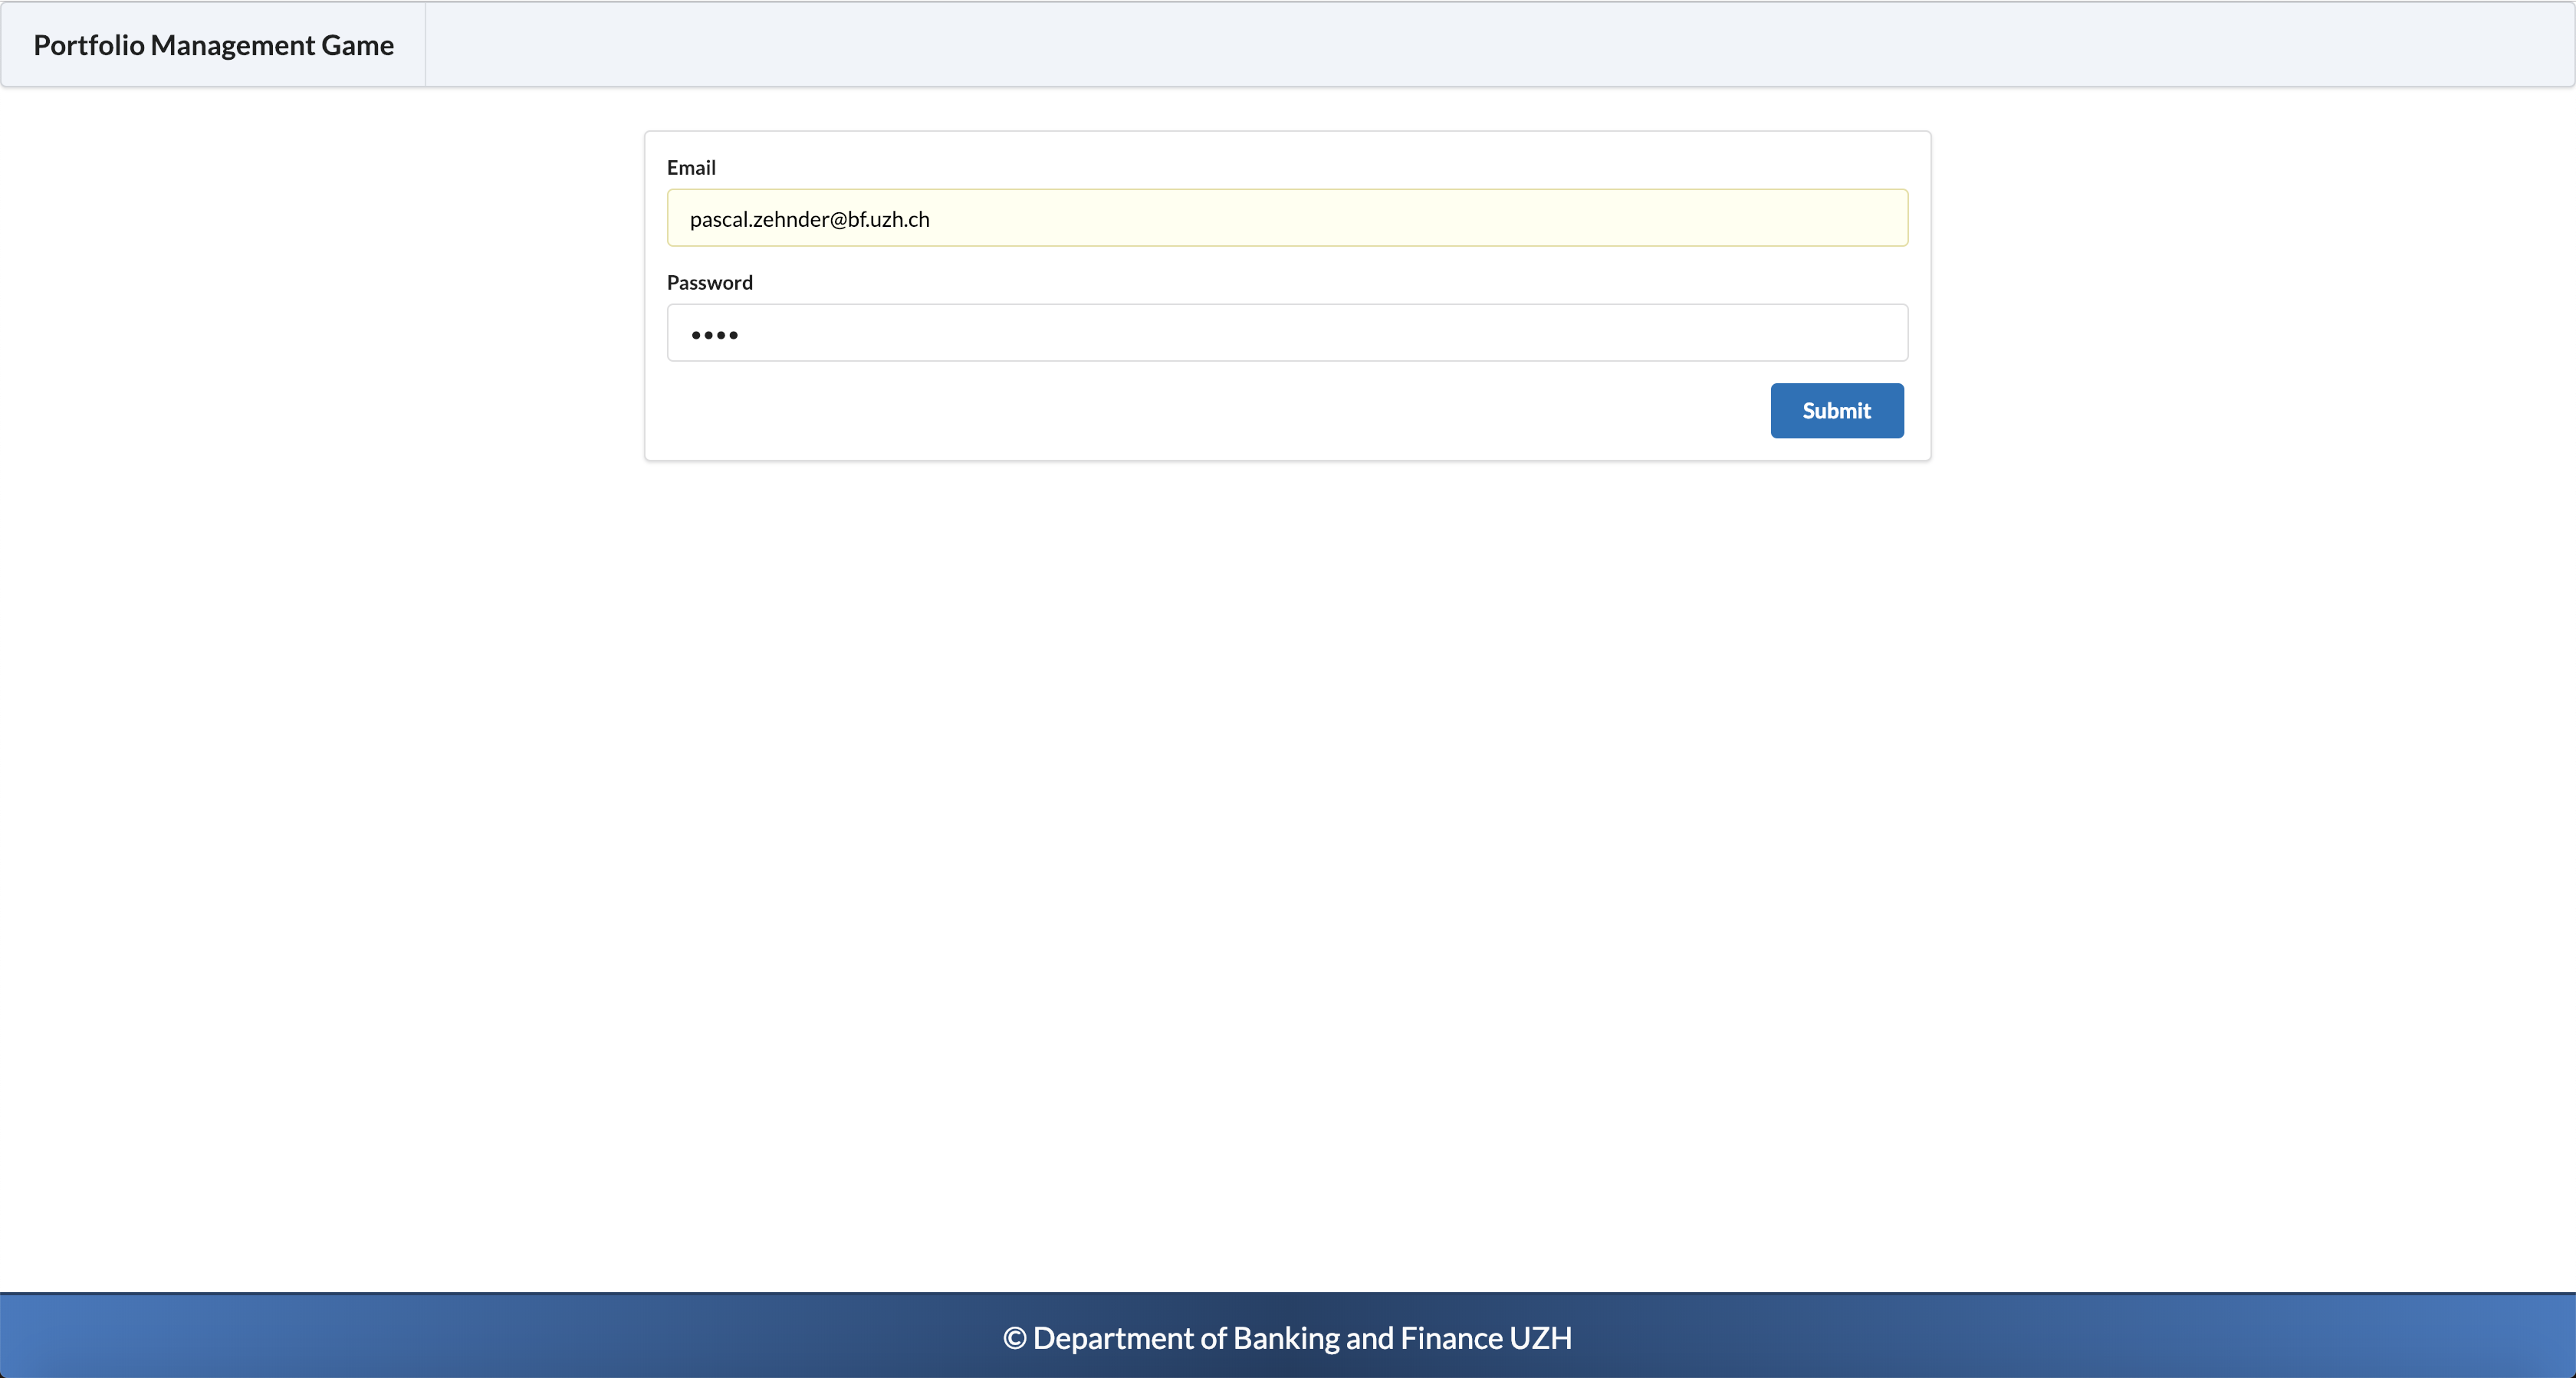
\includegraphics[scale=0.2]{img/application-overview/administrator/01_login.png}
  \caption{Administrator login}
\end{figure}

\subsubsection{Game management}
\paragraph{Game overview}
\label{paragraph:game_overview}
As for landing page of the administrator the game overview exists. It serves as the control center of the game administration. Multiple games can be maintained simultaneously by one game master. Some instant information identifies the current progress of the game within the list, such as game name, short game id or the phase of the game.
\begin{figure}[h!]
  \centering
  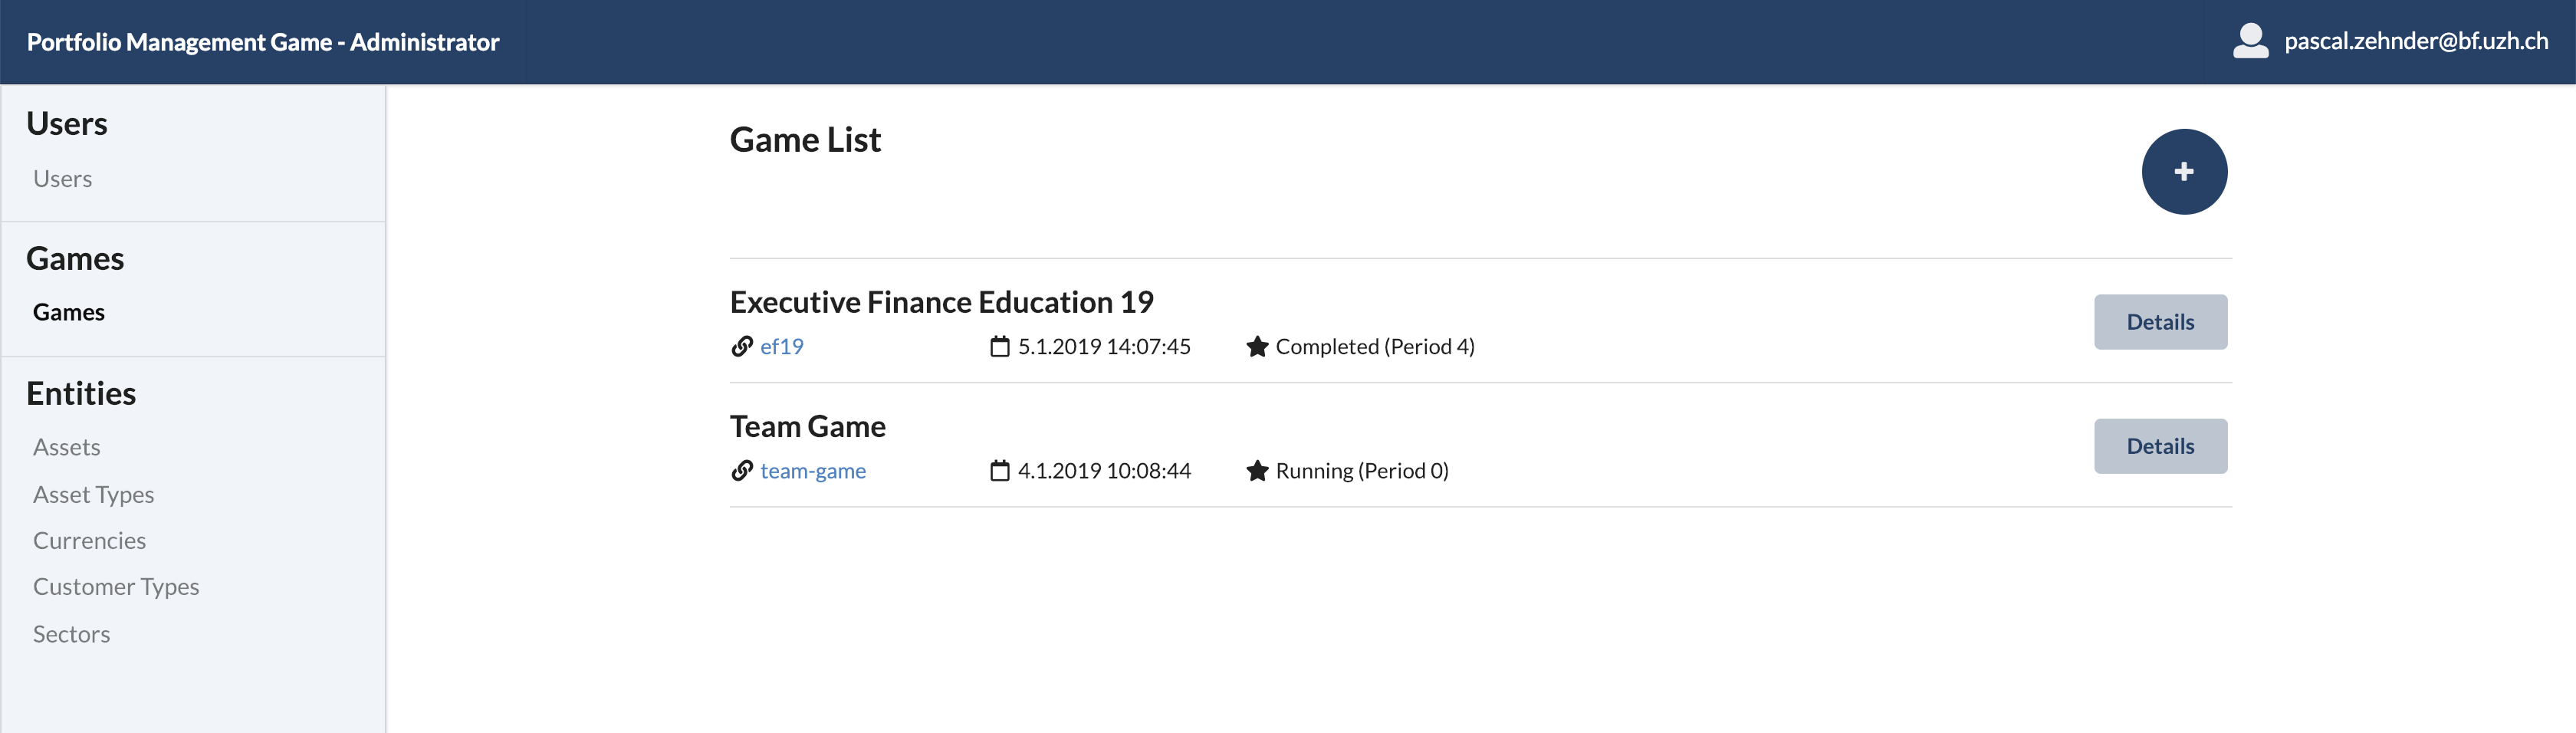
\includegraphics[scale=0.2]{img/application-overview/administrator/02_game_overview.png}
  \caption{Game overview}
  \label{fig:game_overview}
\end{figure}

\paragraph{Game creation}
For creating a game the administrator needs to define some parameters, by filling out a form which is structured into three steps. By pressing on the ''next''-button the administrator will be led through the form. Some tooltips help users to understand the purpose of the provided input. After submitting the creation of the game, the user will be redirected to the game detail of the newly created game.
\begin{figure}[h!]
  \centering
  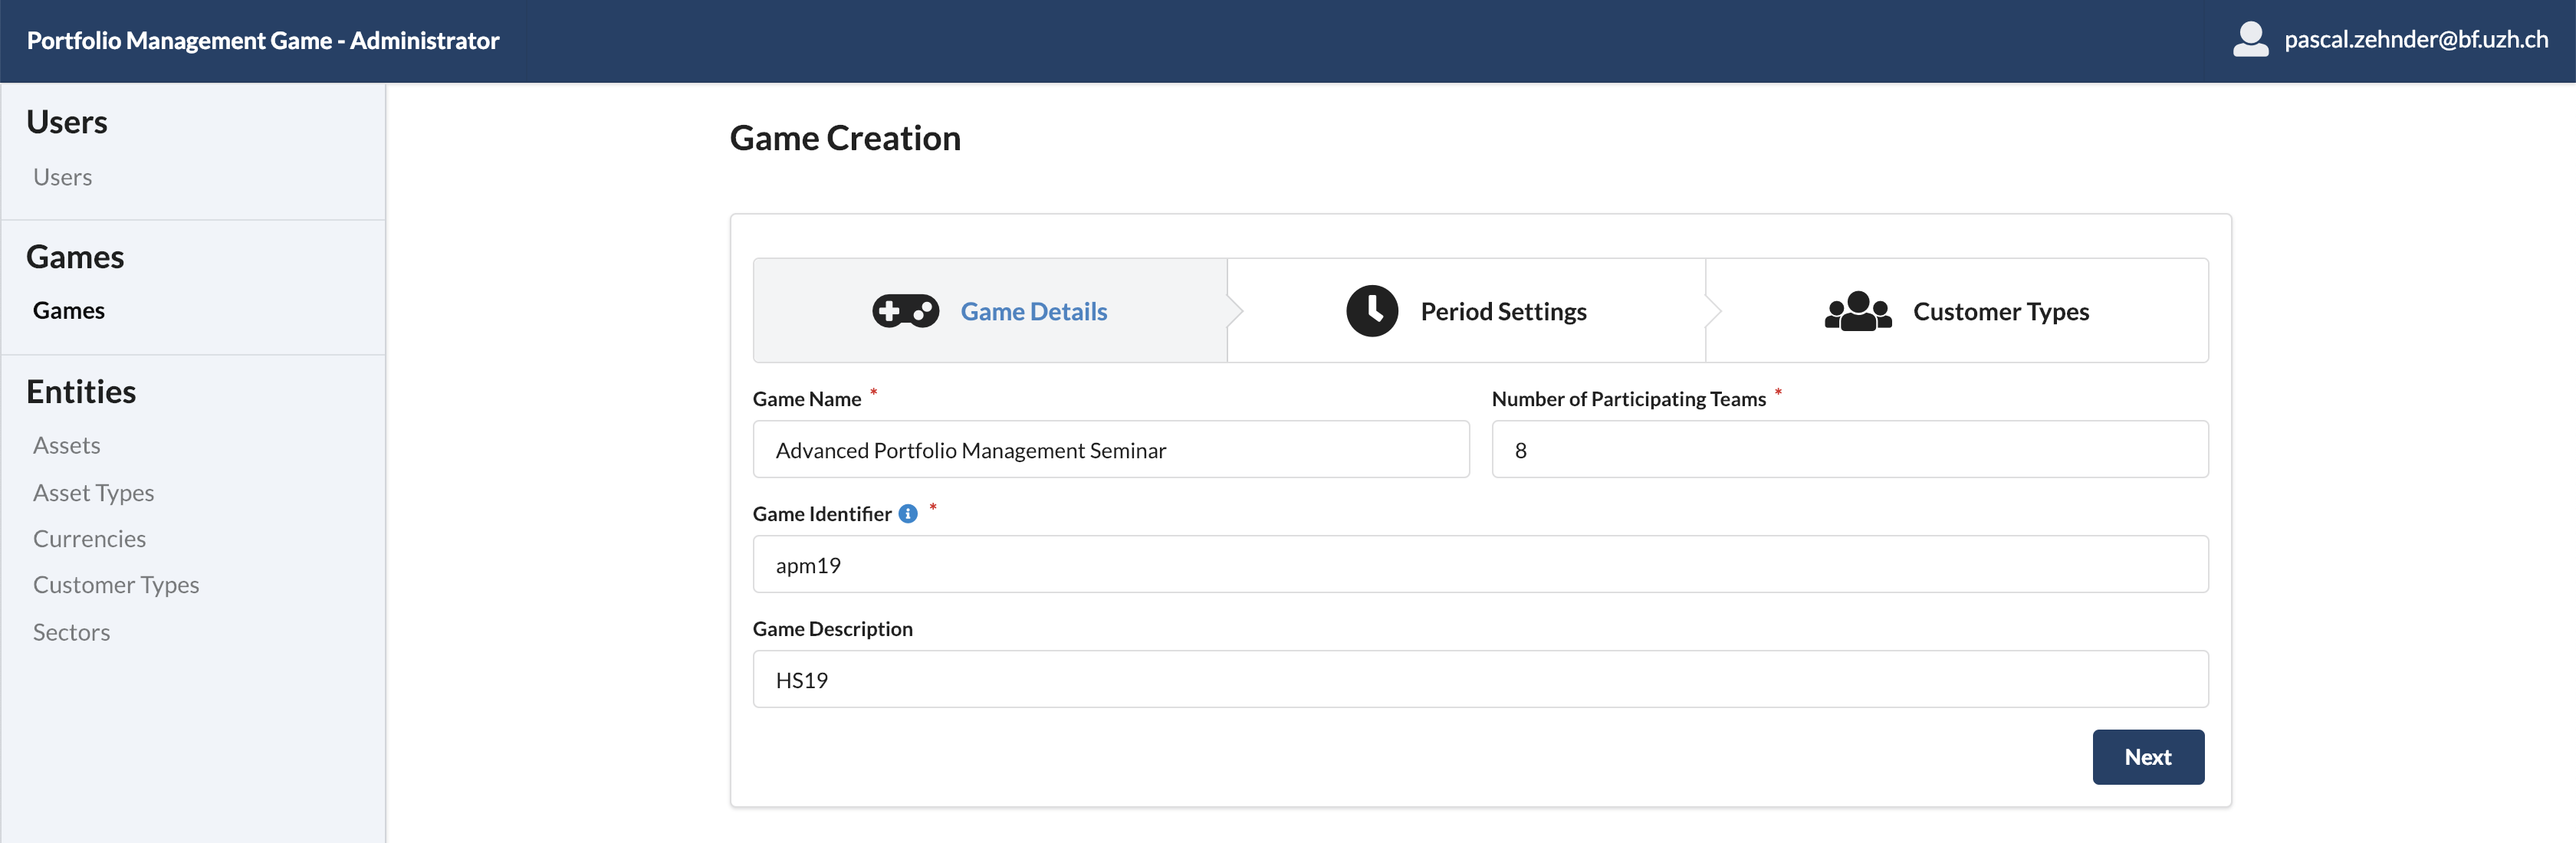
\includegraphics[scale=0.2]{img/application-overview/administrator/03_game_creation.png}
  \caption{Game creation}
\end{figure}


\paragraph{Game detail}
The game detail for each game may be accessed over the game overview list, as seen in figure~\ref{fig:game_overview}. In this page a user can initialize period, start periods, have an overview of the teams' submission and many other features, which will be described in this paragraph:

\subparagraph{Game initialization}
As the game creation may be done in advance we have split the game creation from the game initialization, such that last adjustments of the game may be done just before the start of the game.
\begin{figure}[h!]
  \centering
  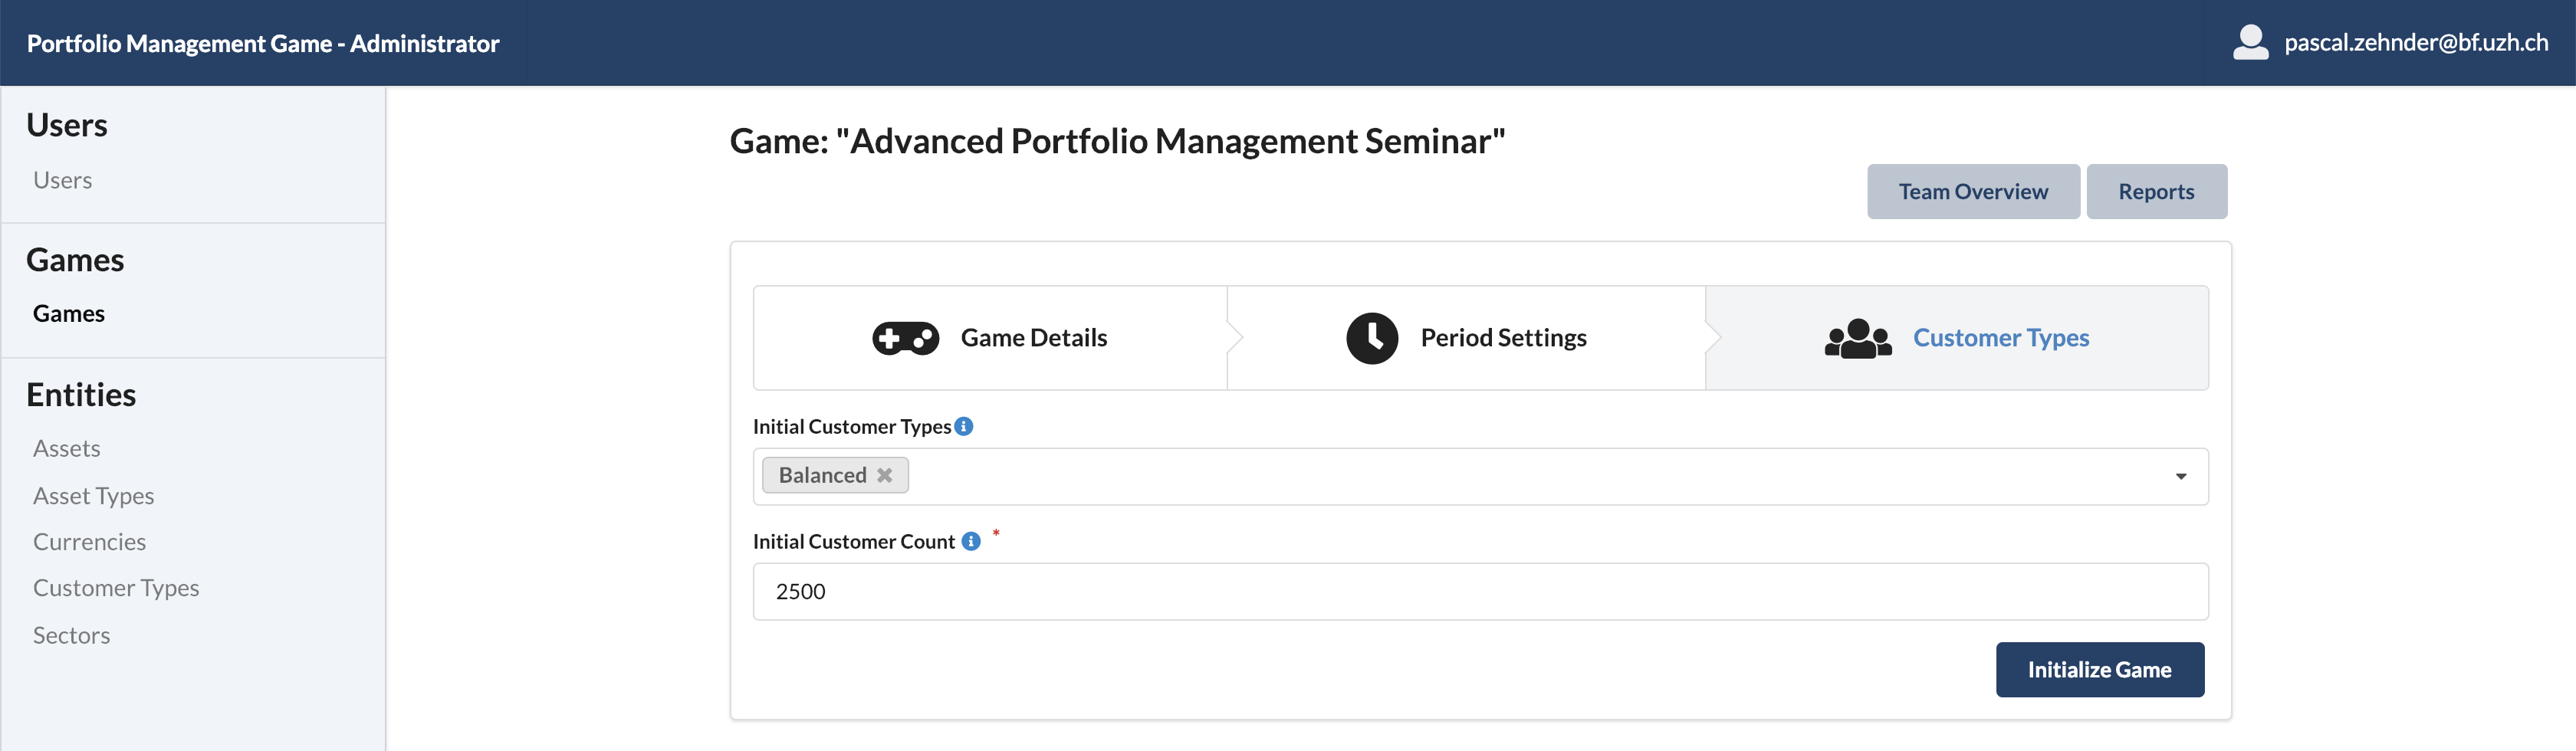
\includegraphics[scale=0.2]{img/application-overview/administrator/04_game_initialization.png}
  \caption{Game initialization}
\end{figure}

\subparagraph{Game start}
By starting the game the students or teams are finally able to start with their period zero decisions. Administrators are able to give them some help over messages which will be visible for the teams in their report section by creating customizable messages. Figure~\ref{fig:game_start} shows a game which is still planned and may be started next.
\begin{figure}[h!]
  \centering
  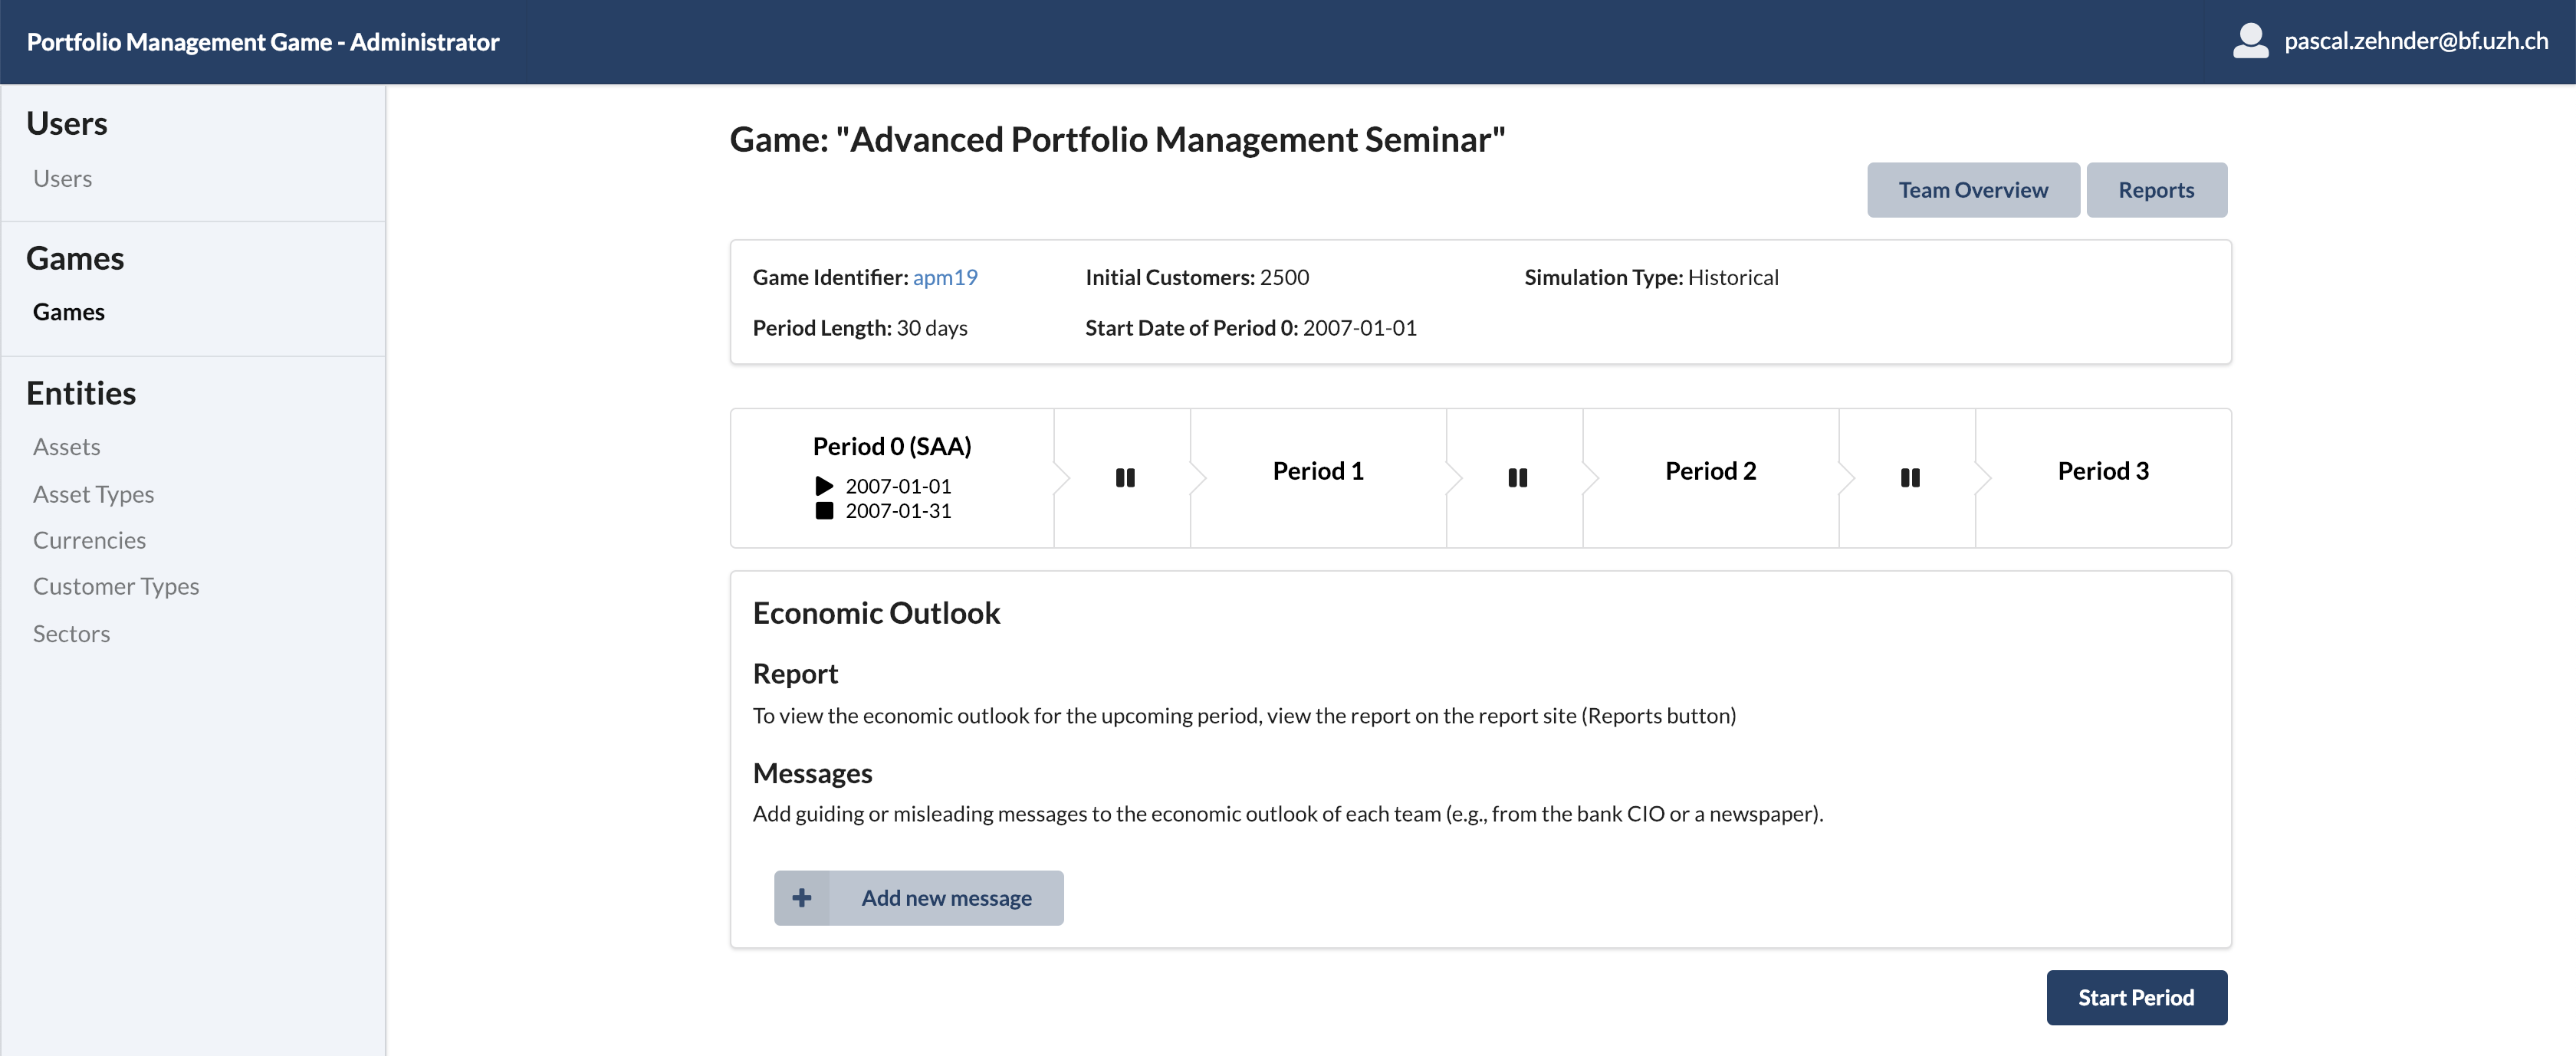
\includegraphics[scale=0.2]{img/application-overview/administrator/05_game_start.png}
  \caption{Game start}
  \label{fig:game_start}
\end{figure}


\subparagraph{Team overview}
\label{subparagraph:team_overview}
For providing access for all teams an administrator has an overview about the team logins (figure~\ref{fig:team_overview}), which are generated automatically when initializing a game.
\begin{figure}[h!]
  \centering
  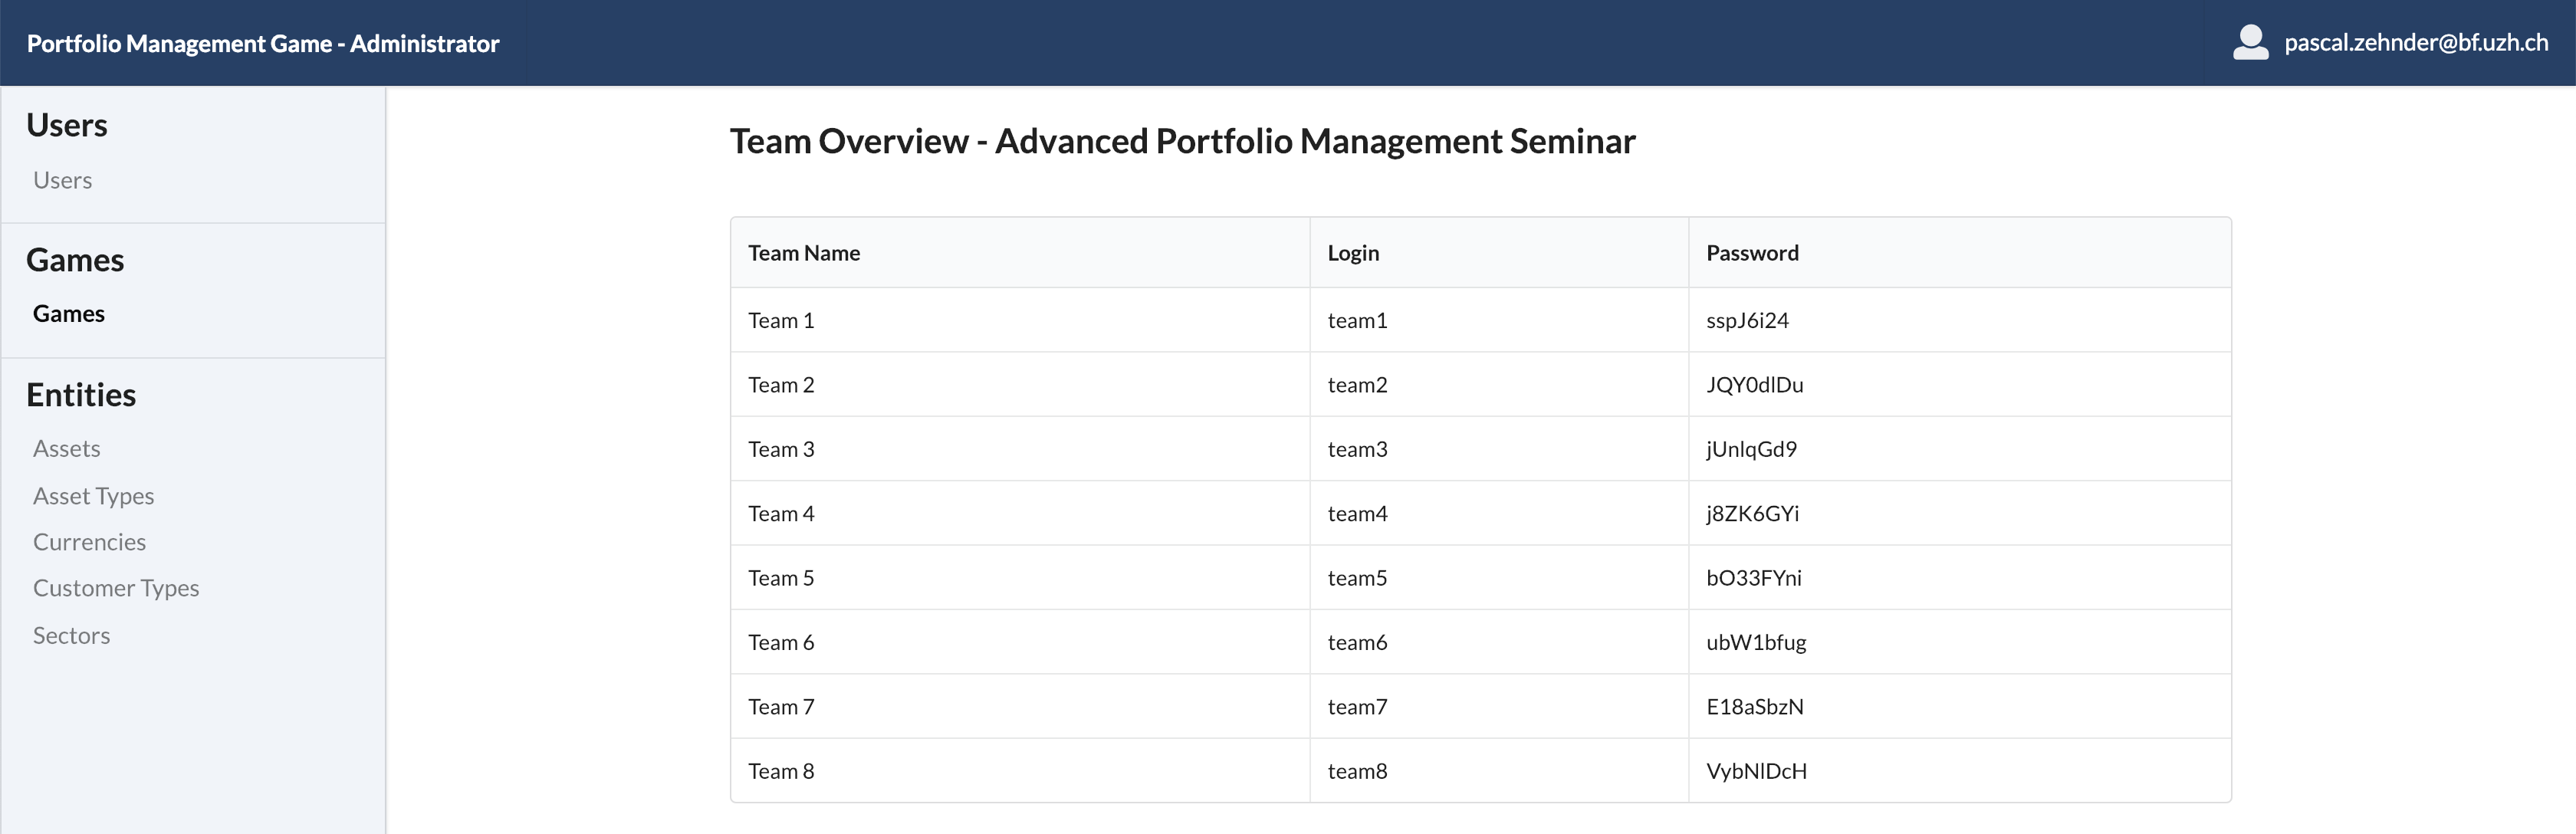
\includegraphics[scale=0.2]{img/application-overview/administrator/06_team_login_overview.png}
  \caption{Team overview}
  \label{fig:team_overview}
\end{figure}

\subparagraph{Running game}
Overview of the submission state of all teams. The administrator is able to get an insight about the decisions of all submitted teams. The period can only be finished if all teams submitted and therefore the state of the teams has been green.
\begin{figure}[h!]
  \centering
  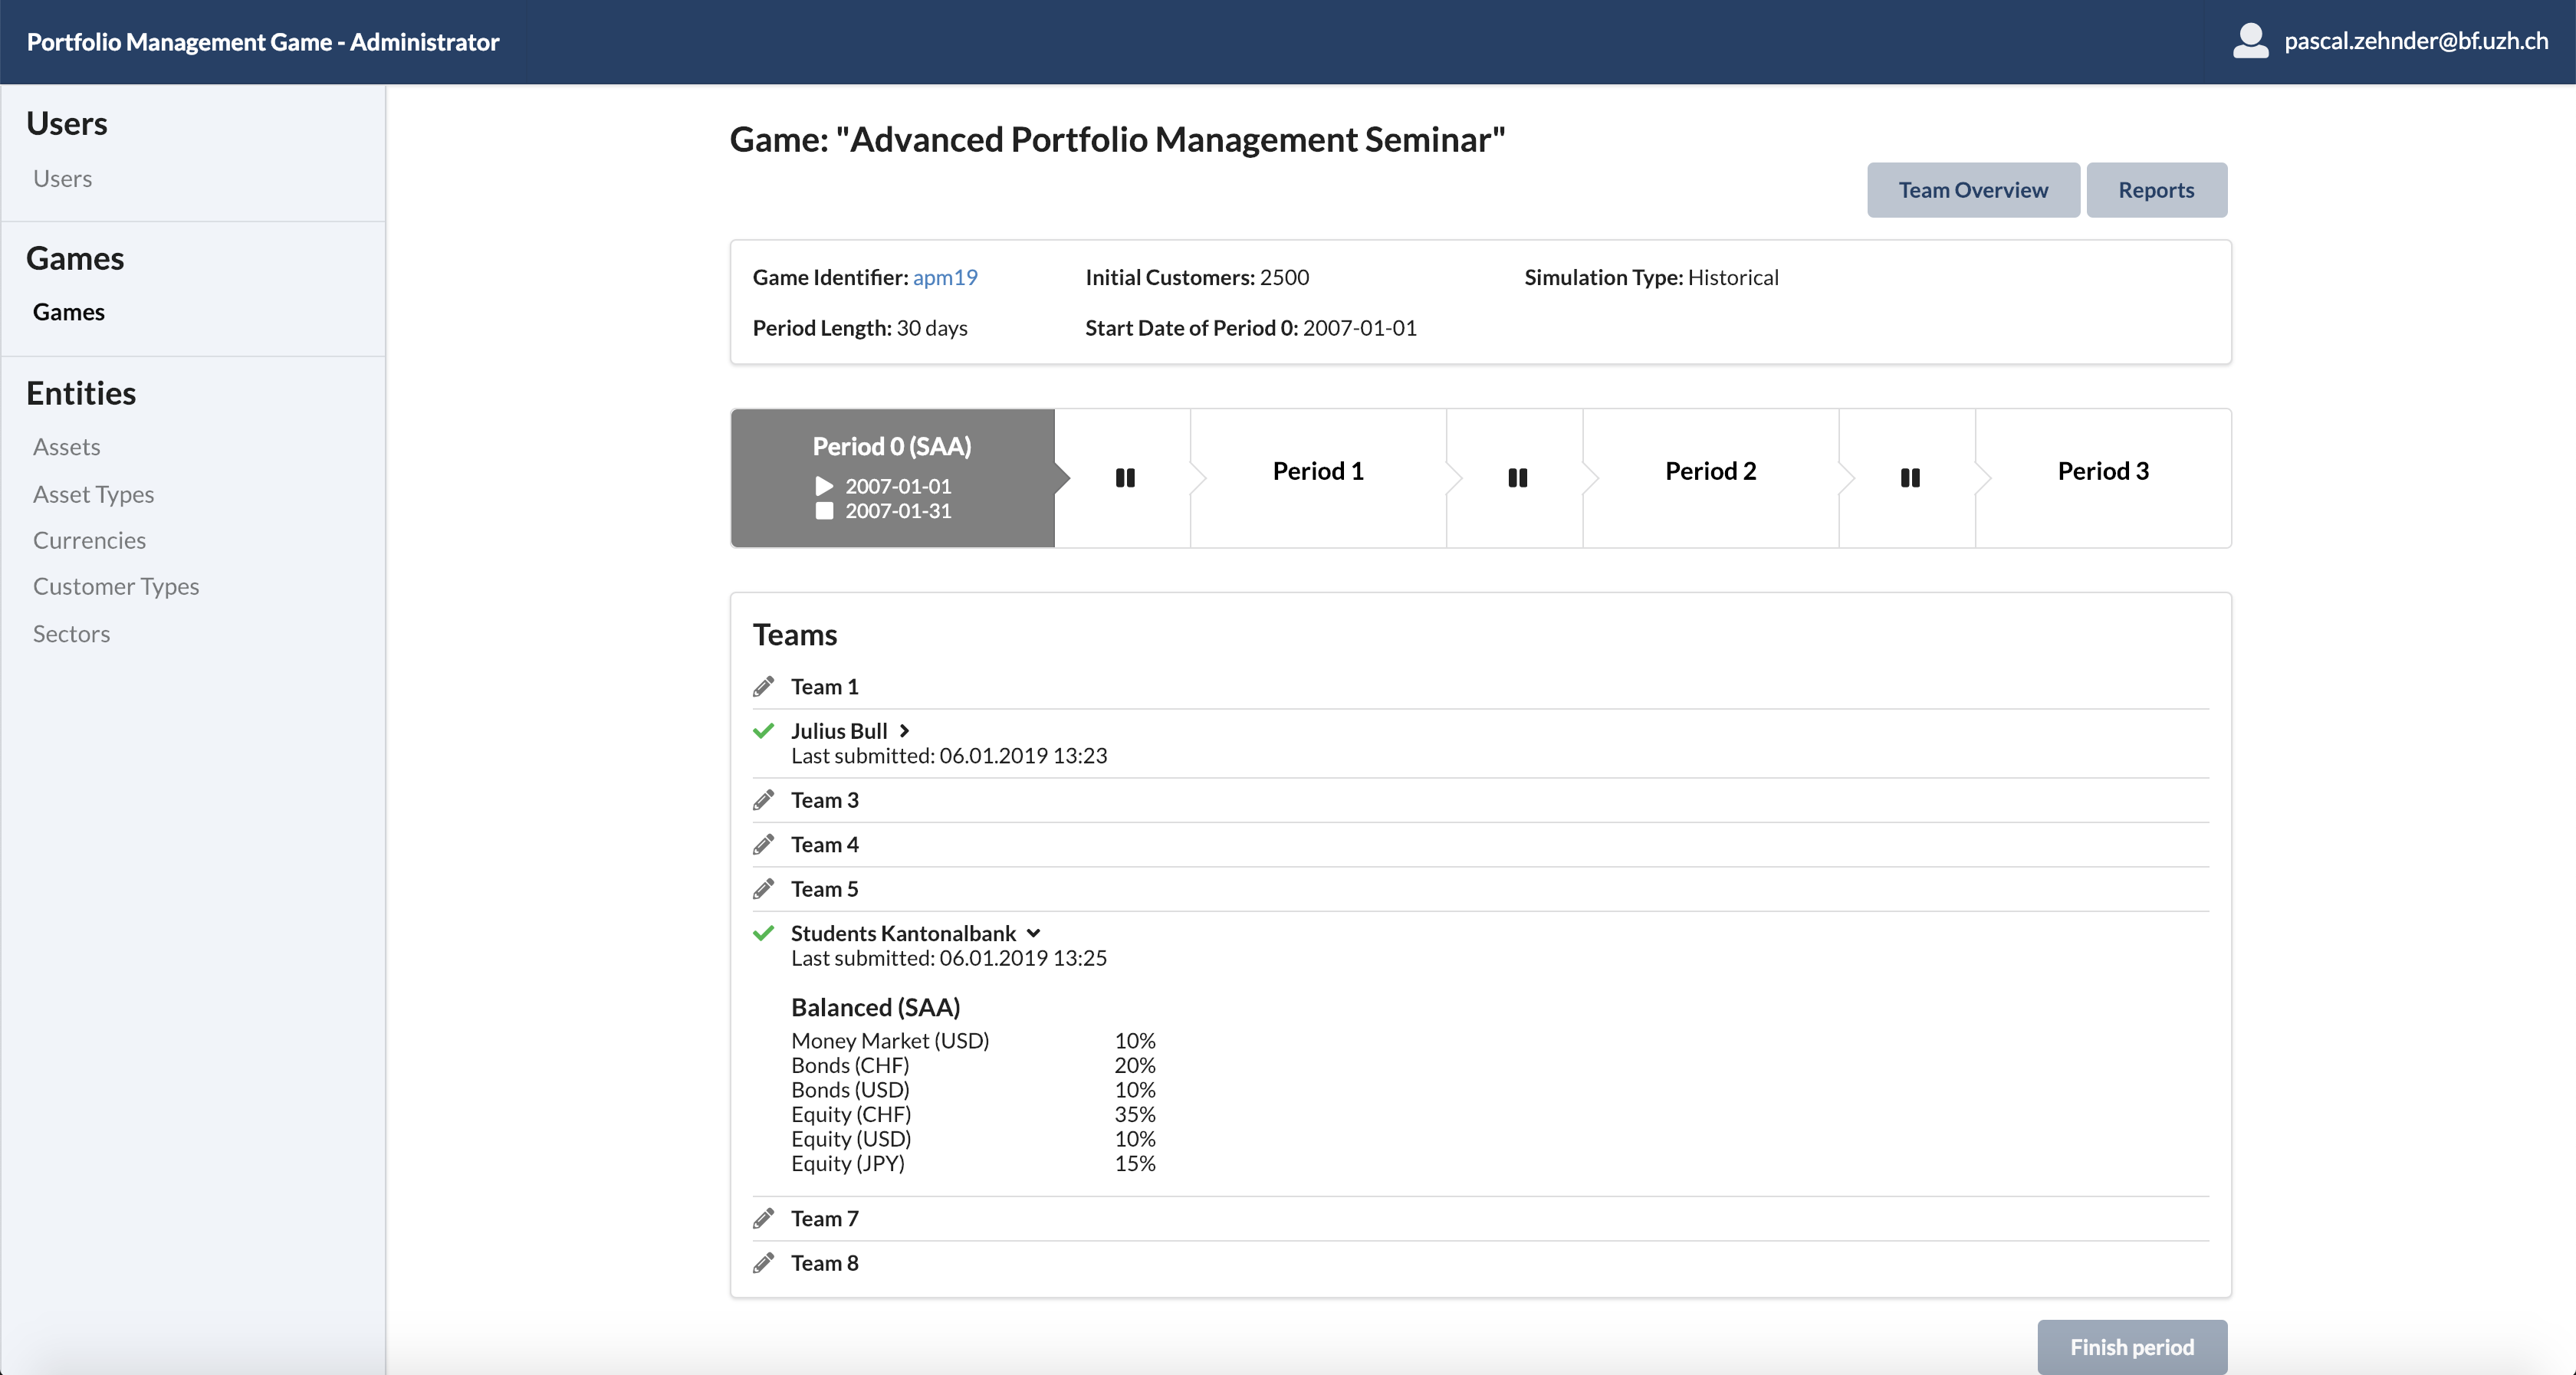
\includegraphics[scale=0.2]{img/application-overview/administrator/07_running_game.png}
  \caption{Running game}
\end{figure}

\subparagraph{Initializing period}
After completion of period zero, the administrator has to initialize a period in which the team decisions will be compared to the other teams decisions and evaluated. Additionally, new customer types for the next period and other settings could be defined in this phase of the game.
% TODO replace with a screen including customer type settings from period 2 e.g.
\begin{figure}[h!]
  \centering
  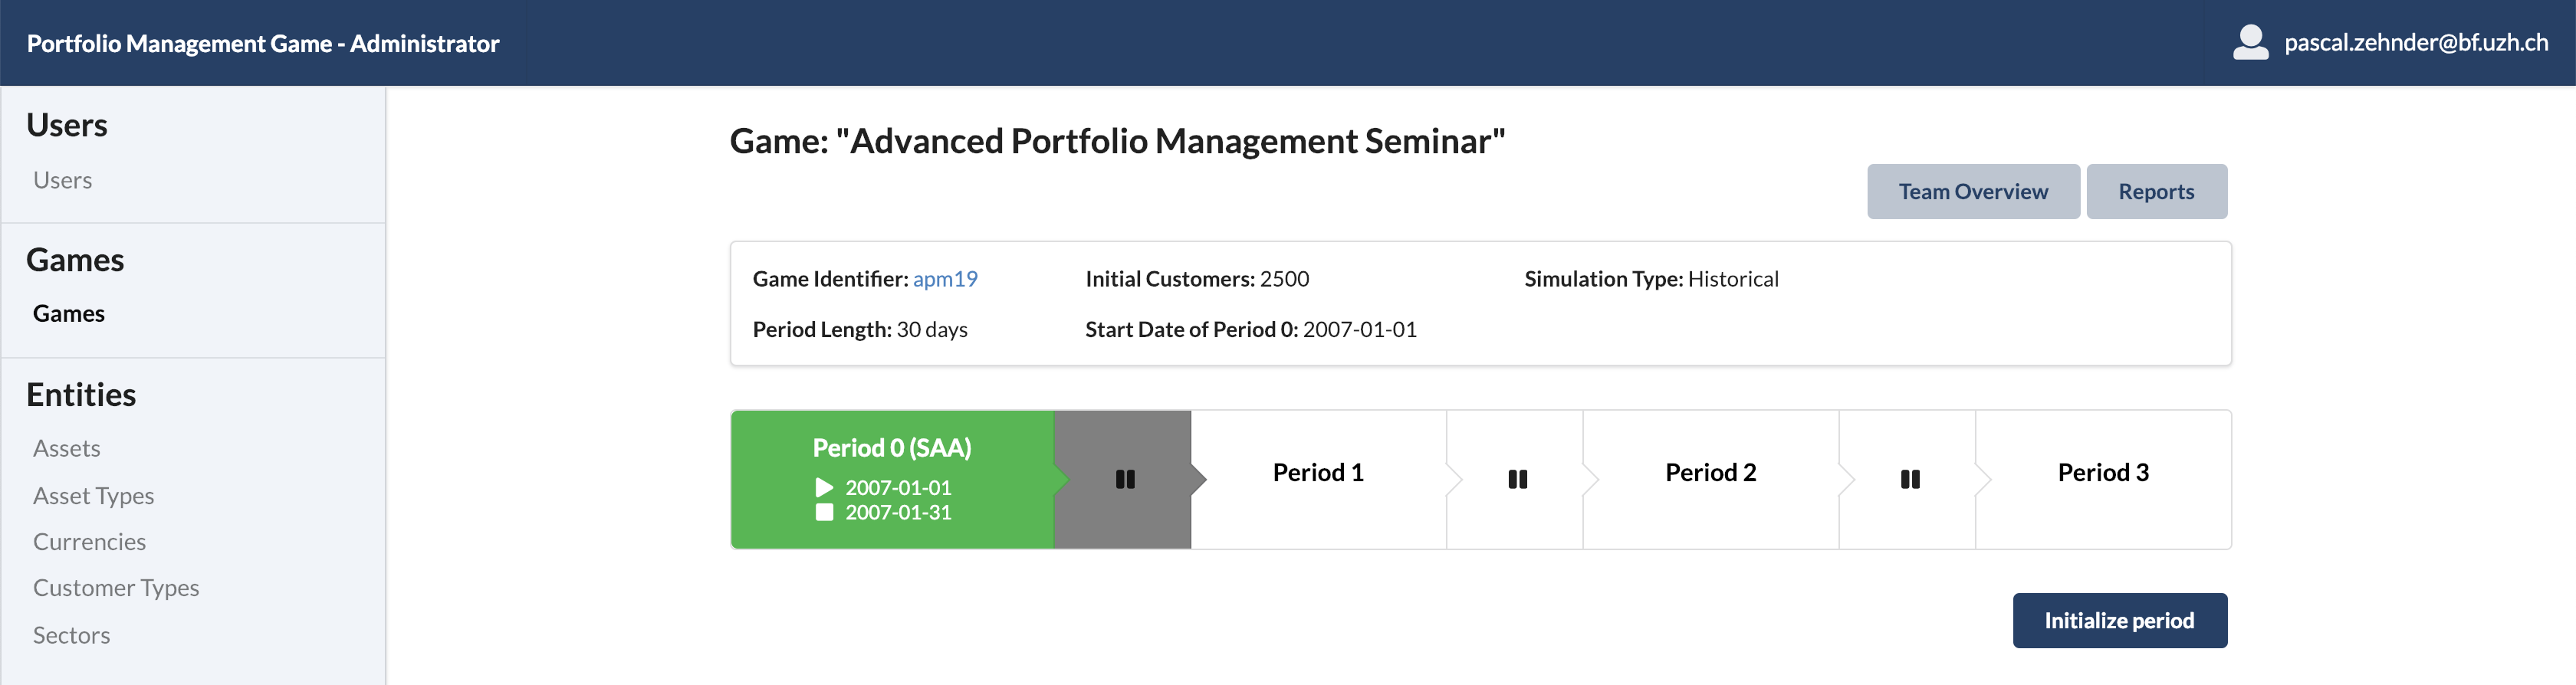
\includegraphics[scale=0.2]{img/application-overview/administrator/08_period_initialization.png}
  \caption{Initialize period}
\end{figure}


\subparagraph{Period start}
By completing the simulation, respectively evaluation of the previous period, a next period may be started. If the game is still paused the teams cannot access the decisions site. The administrator can define some optional messages which will be displayed in the teams report page. Some adjustments to the simulation results will be edited in this phase of the game.
\begin{figure}[h!]
  \centering
  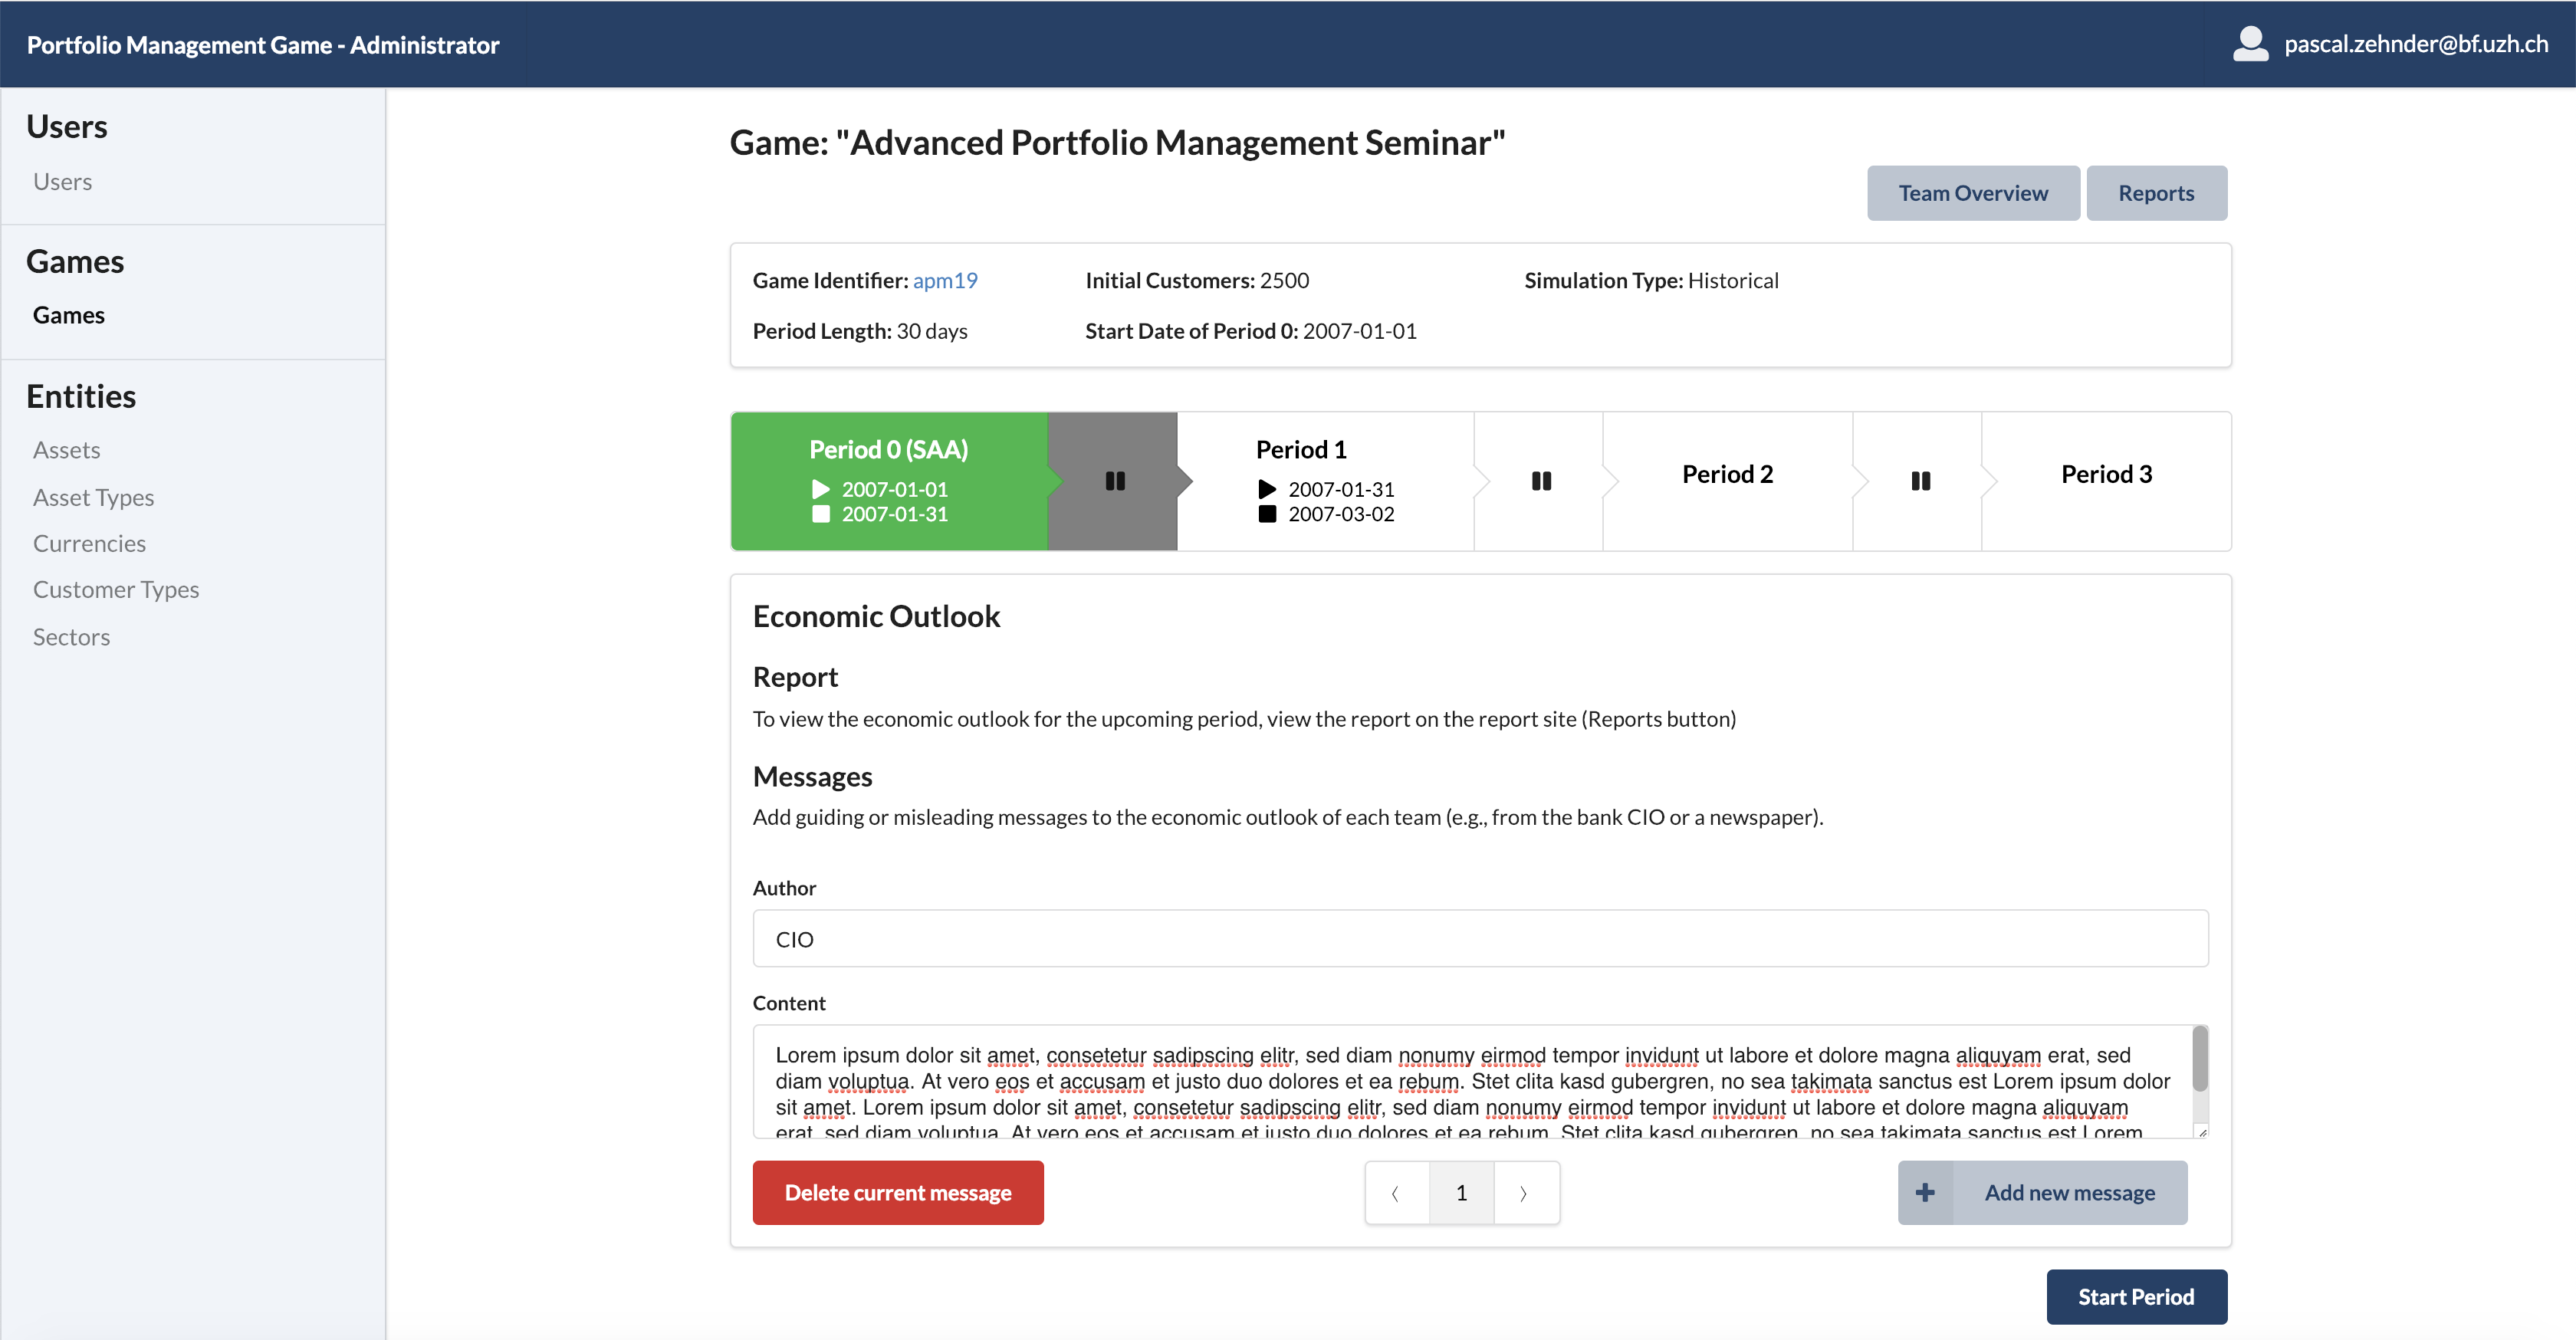
\includegraphics[scale=0.2]{img/application-overview/administrator/09_period_start.png}
  \caption{Period start}
\end{figure}

\subsubsection{Reports}
For the presentation of the teams result in between two running periods being played, a report is accessible for the administrator. A more detailed description will be in section X, as the teams access the same reports as the administrator.


\subsubsection{Entities administration}

\paragraph{Assets}
All assets are visible within this page. They can be synchronized to the current definition within the market repository. % TODO on what?
\begin{figure}[h!]
  \centering
  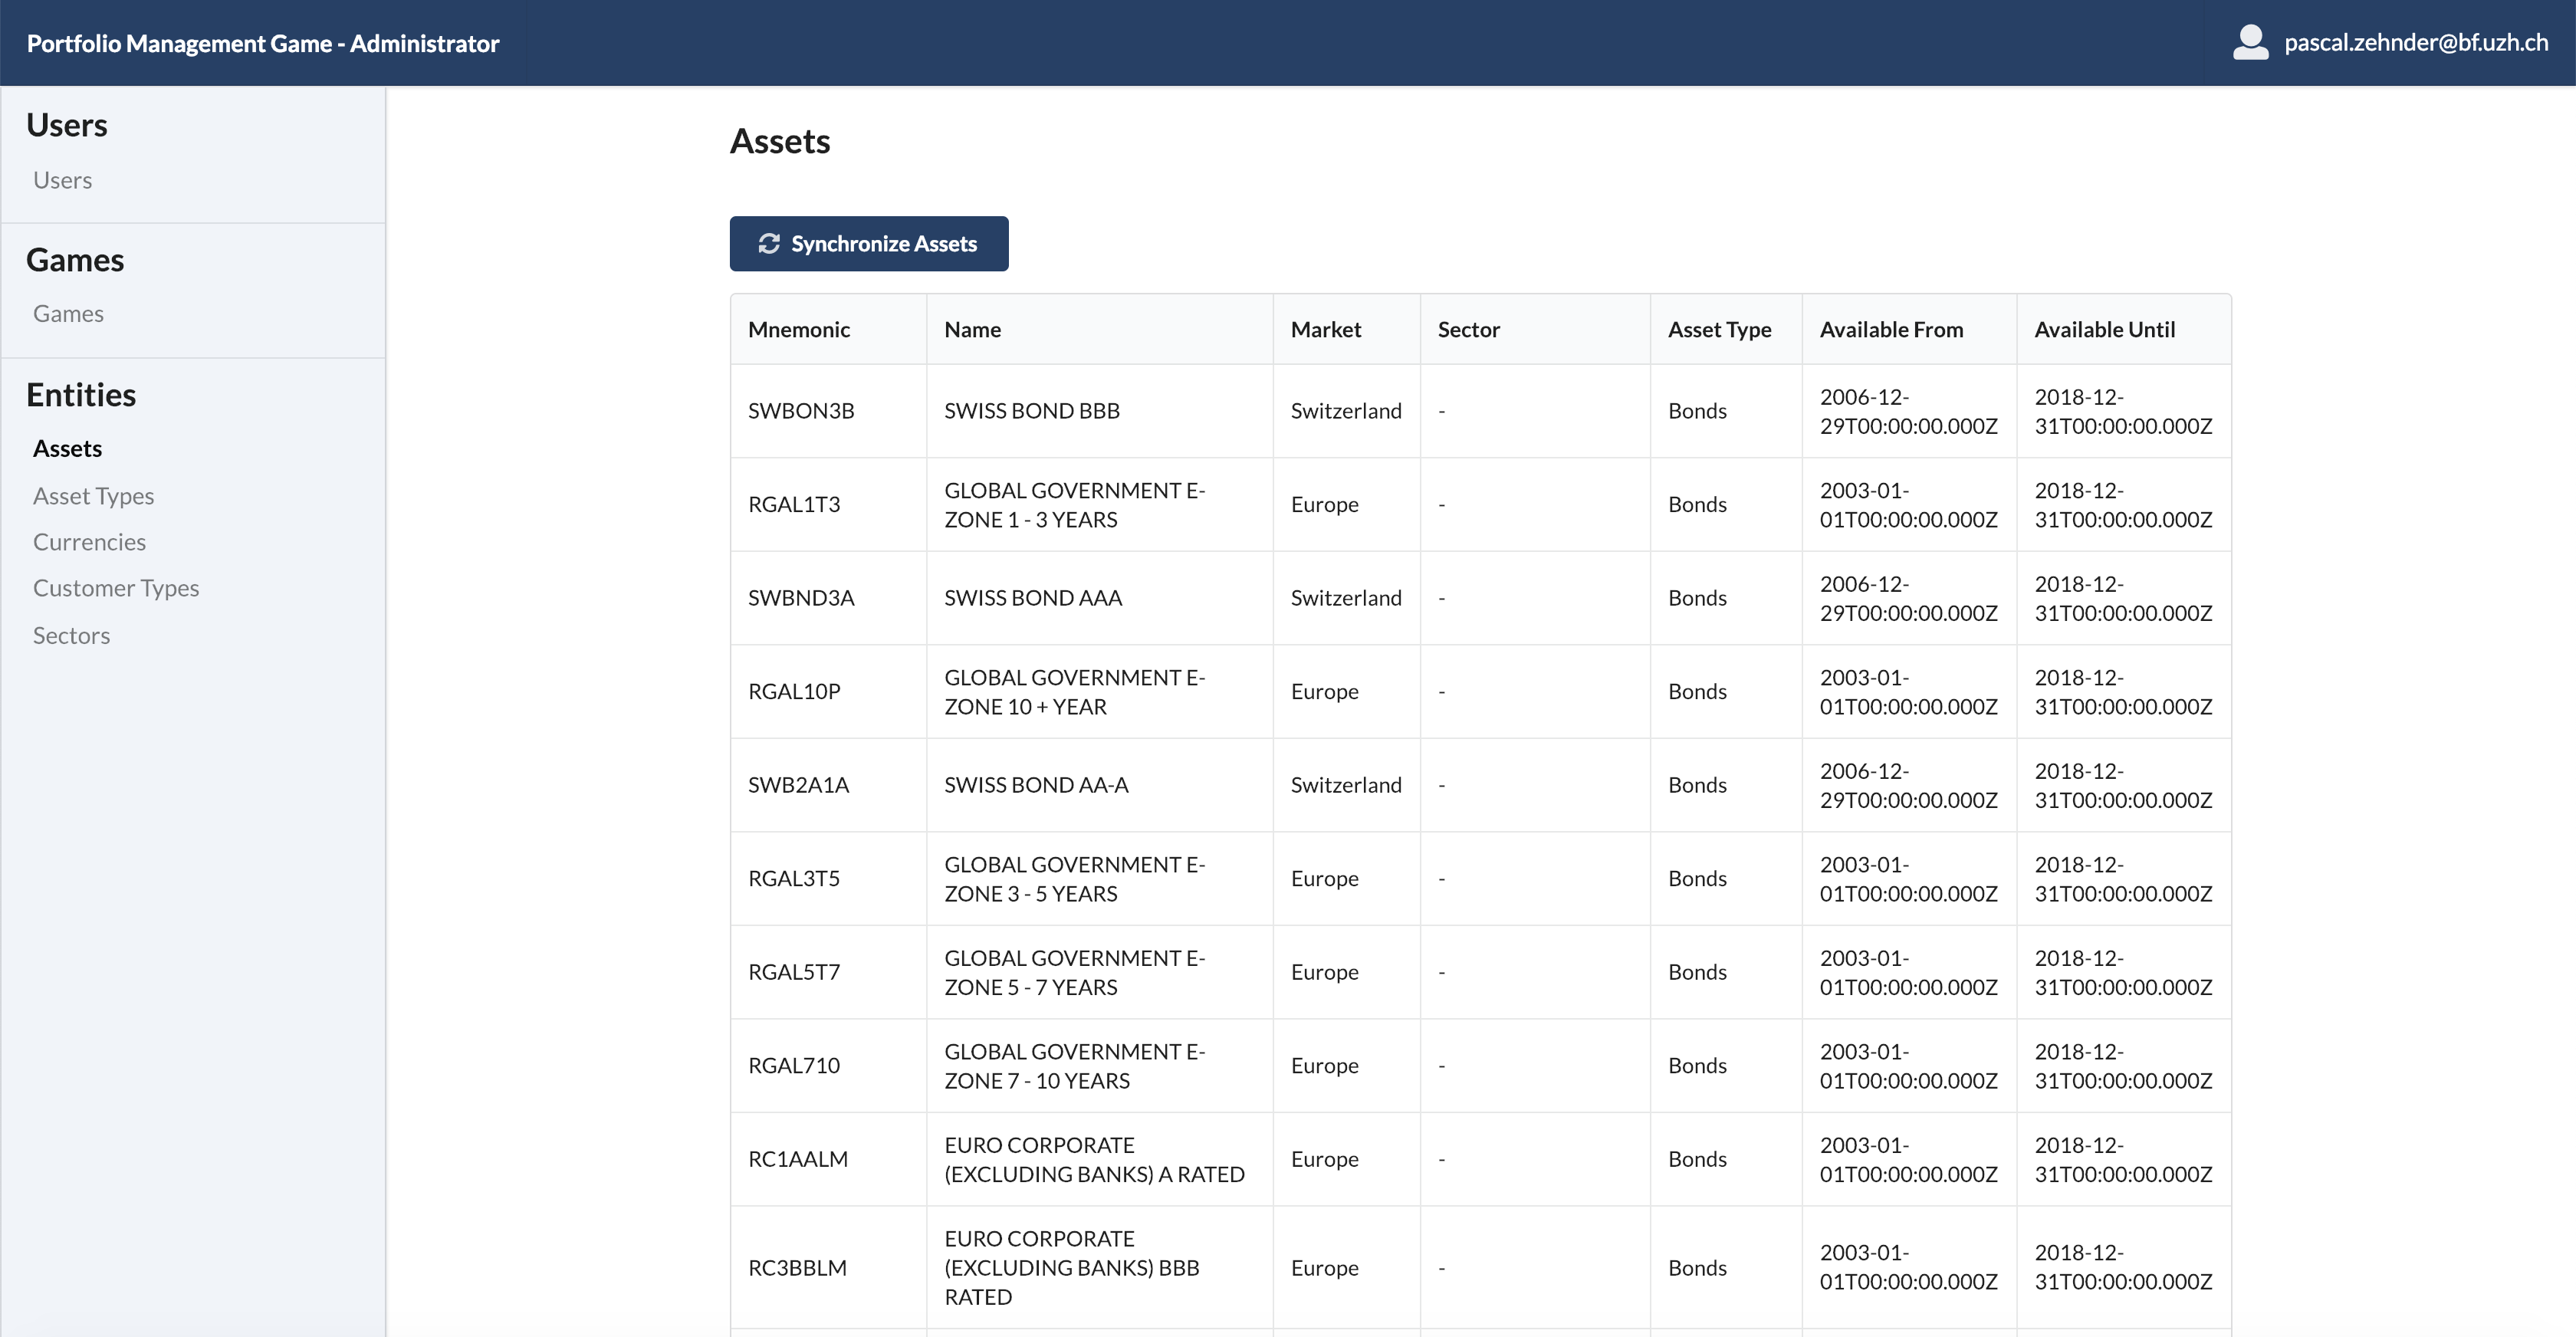
\includegraphics[scale=0.2]{img/application-overview/administrator/entities_assets.png}
  \caption{Assets administration}
\end{figure}


\paragraph{Asset Types}
A table showing all asset types which may be edited is the landing page of this entity. By editing a specified asset type the administrator can change some characteristics of its type, such as info text as shown in figure~\ref{fig:asset_types}.
\begin{figure}[h!]
  \centering
  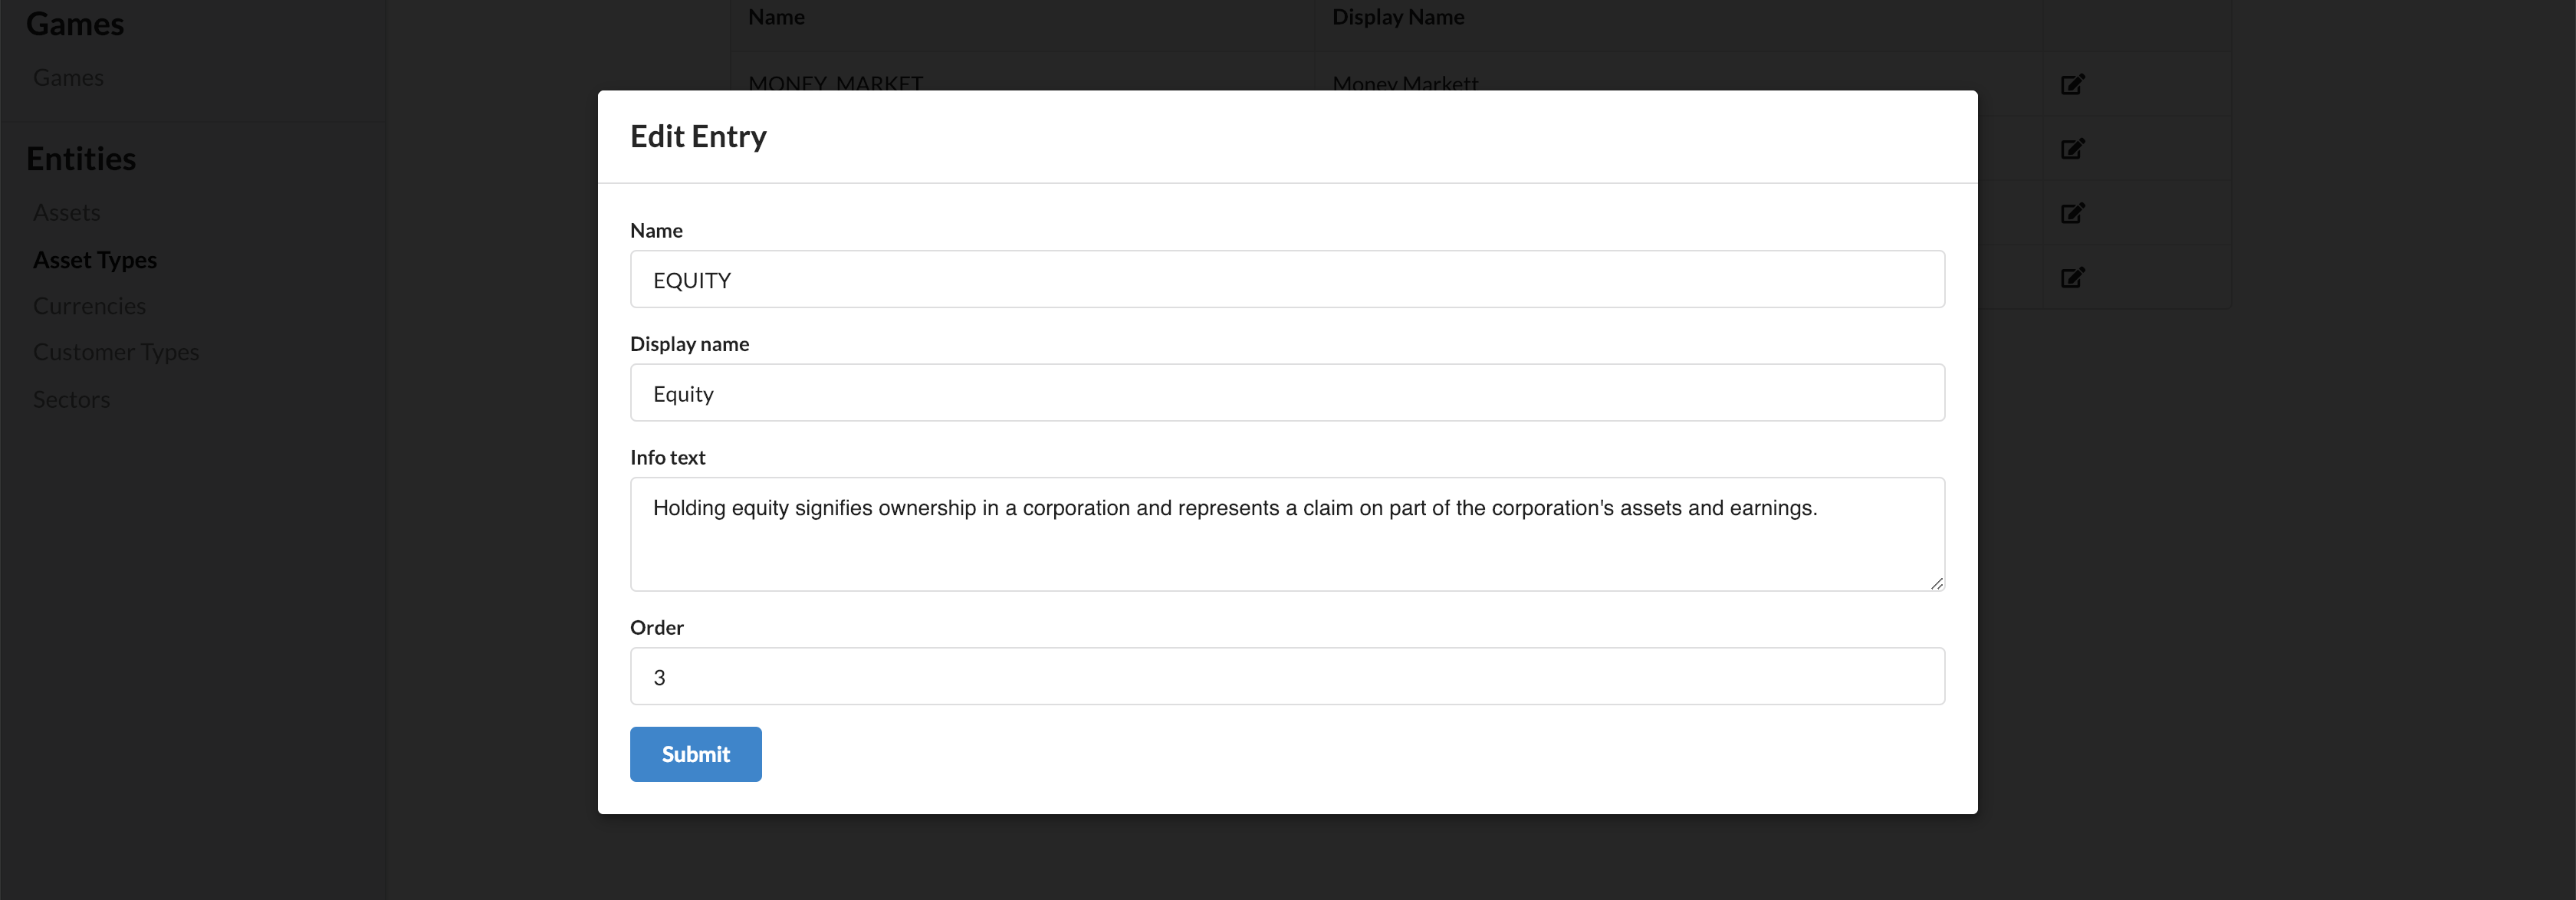
\includegraphics[scale=0.2]{img/application-overview/administrator/entities_asset_types.png}
  \caption{Asset types administration}
  \label{fig:asset_types}
\end{figure}

\paragraph{Currencies}
The currencies may be edited in the same manner as the asset types. By submitting the displaying name or symbol of the corresponding currency may be changed.

\paragraph{Customer Types}
An overview of all in the game available customer types is provided for the administrator. For each customer type, the ideal strategic asset allocation and the ranges for currencies and asset types (both dimensions) can be modified. Additionally, the info bullets and the displaying name may be modified too.
\begin{figure}[h!]
  \centering
  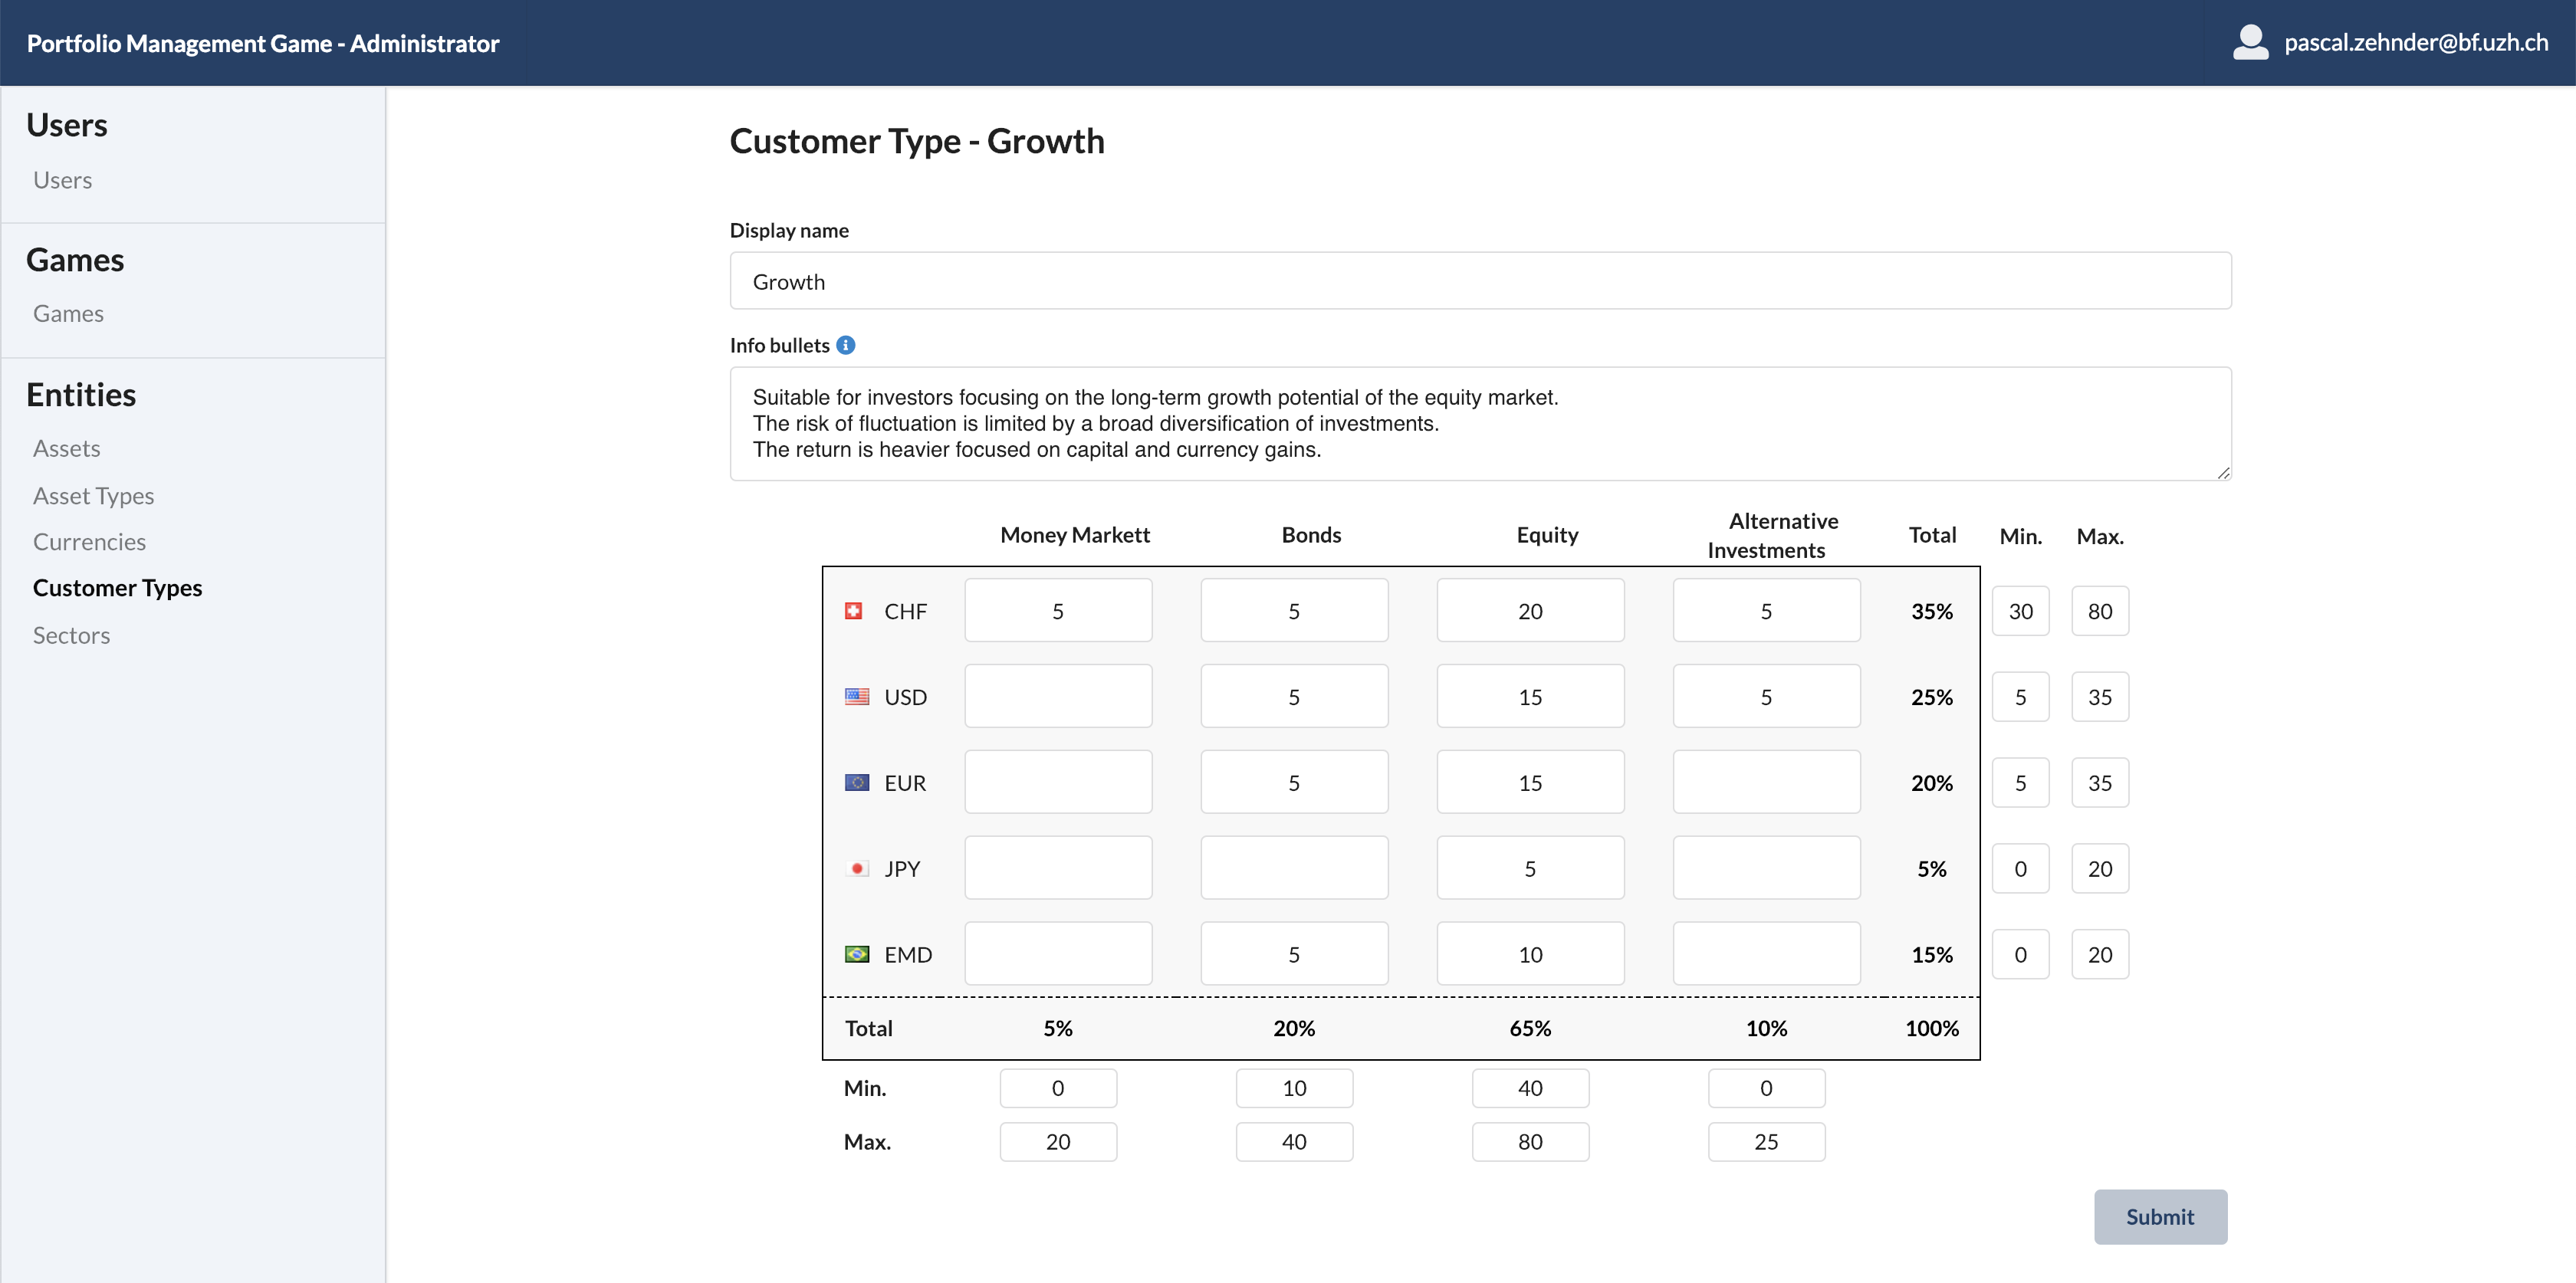
\includegraphics[scale=0.2]{img/application-overview/administrator/entities_customer_types.png}
  \caption{Customer types administration}
\end{figure}


\paragraph{Sectors}
A short overview of all sectors which are used in the asset overview.





\subsection{Team View}

\subsubsection{Login}
%\begin{center}
%  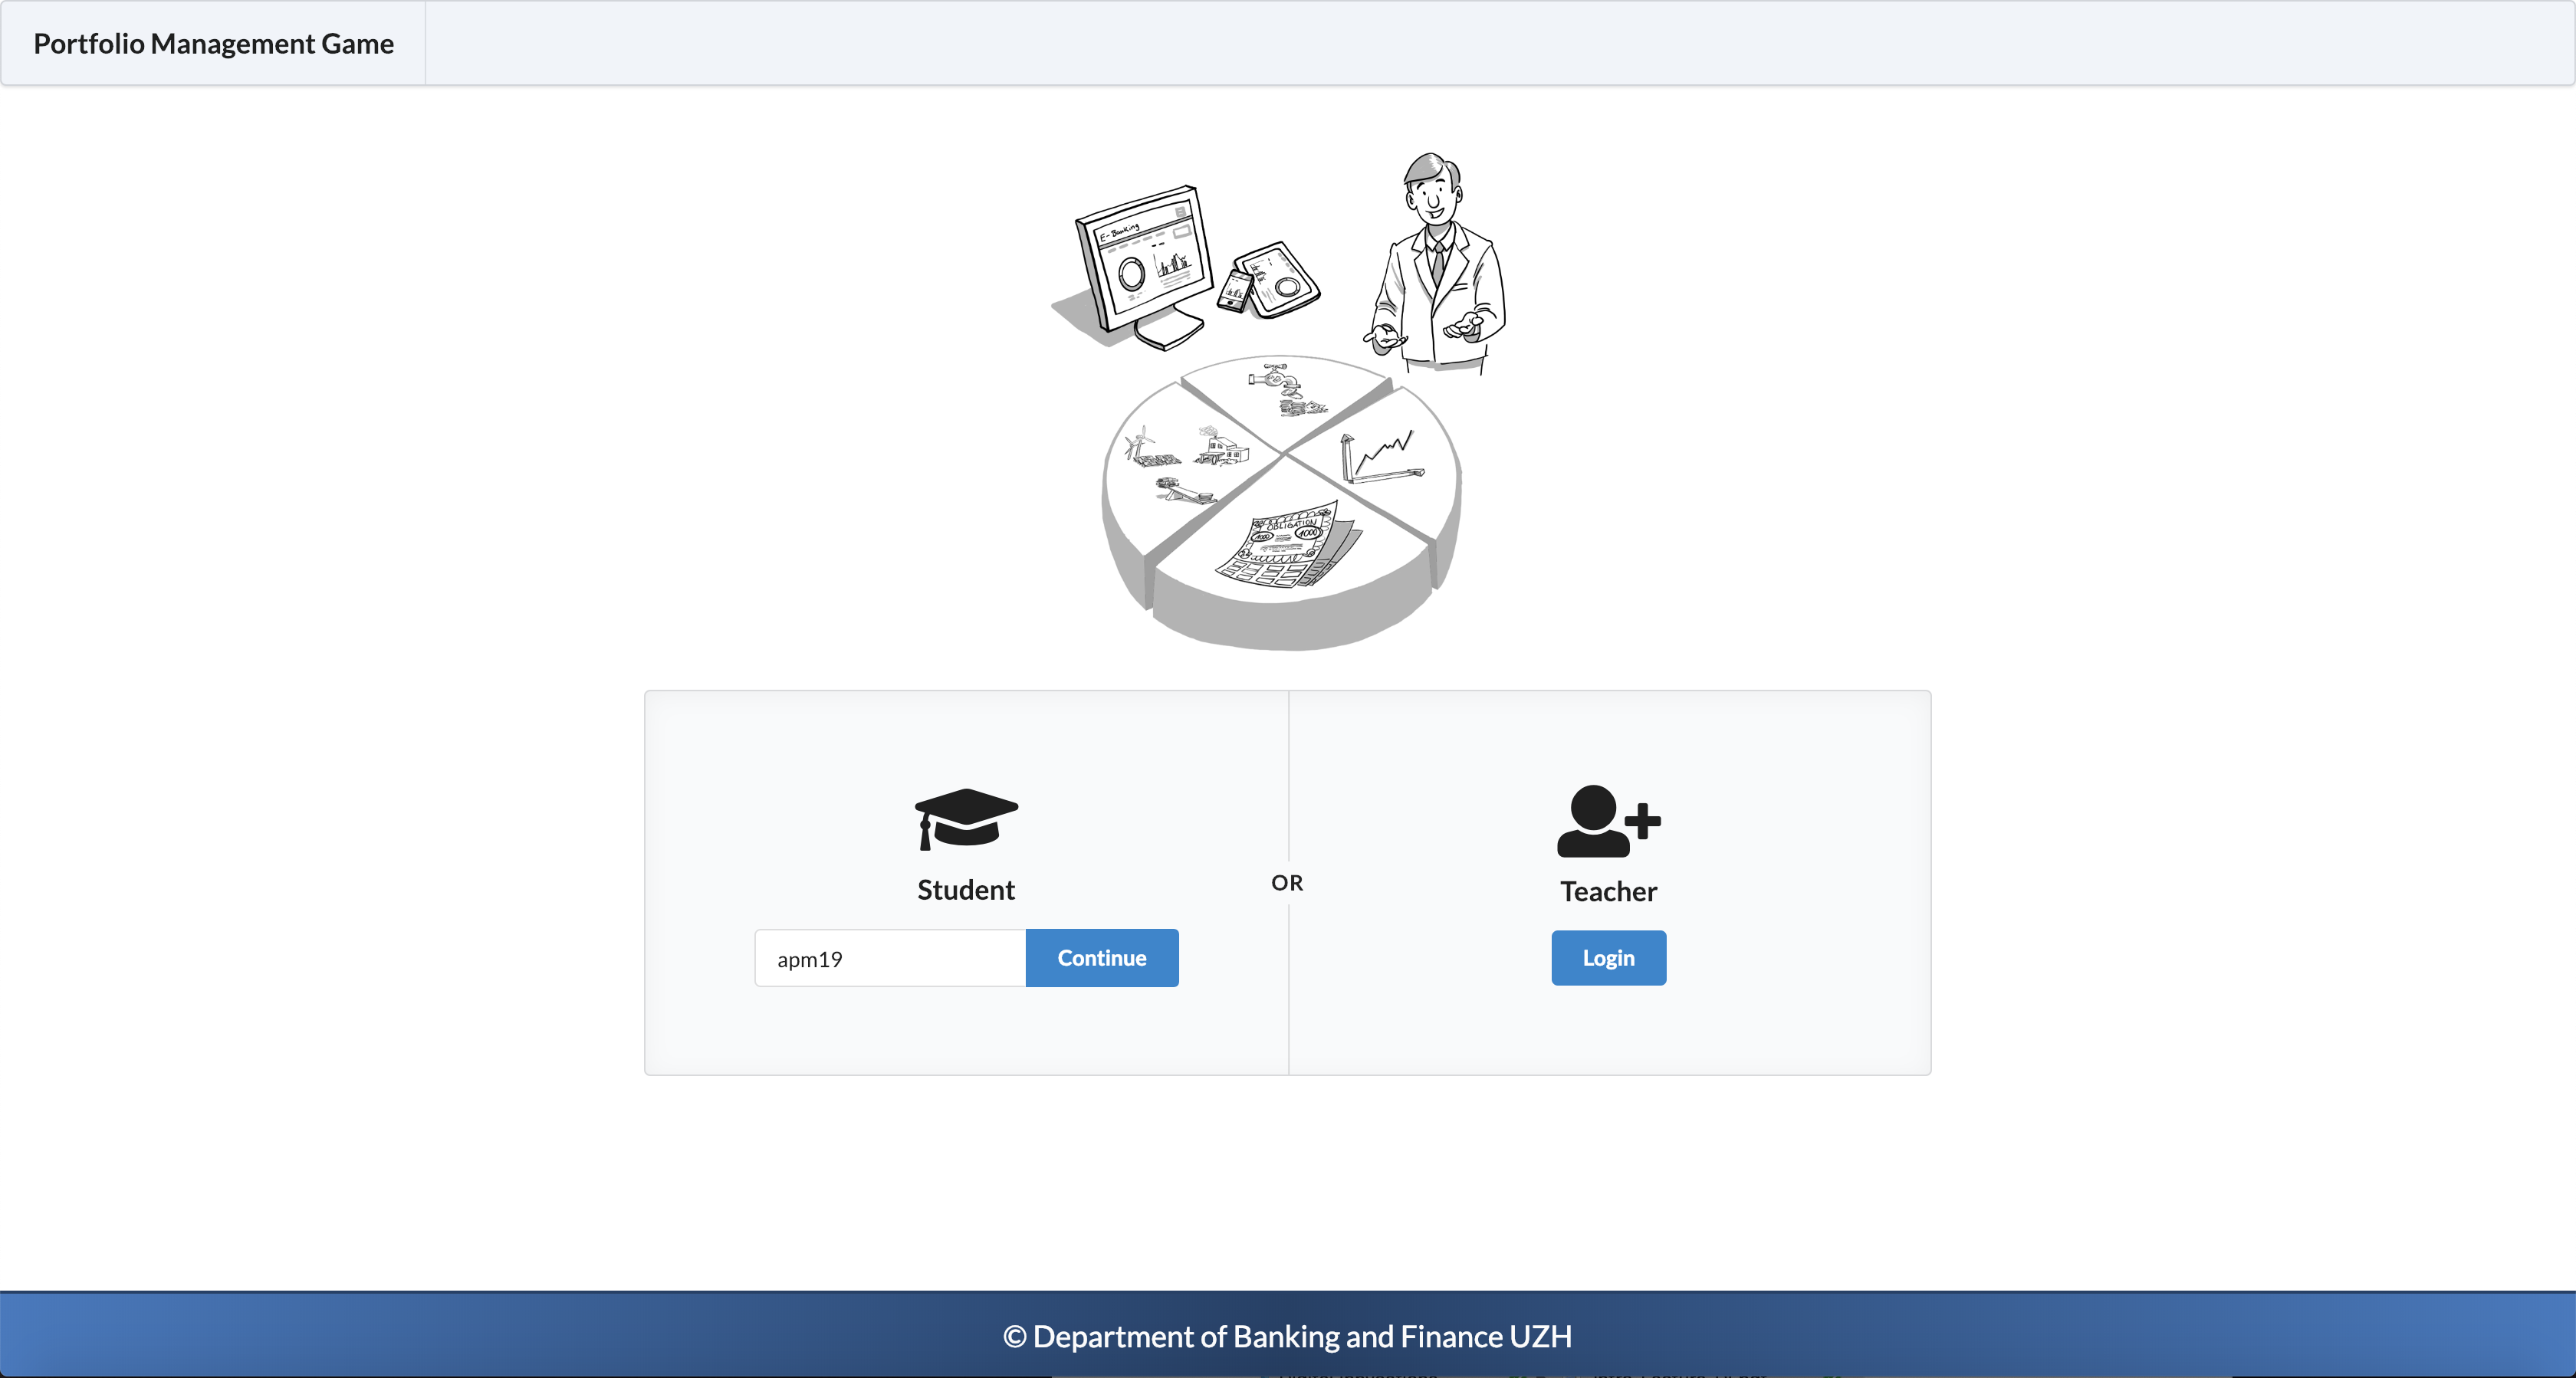
\includegraphics[scale=0.2]{img/application-overview/teams/startpage.png}
%\end{center}
By accessing the starting page, a team has to input a game short id which is provided from the administrator. Afterwards, the team has to login within a correct game identifier to participate within a game. The login credentials are accessible from the administrator screen fro each team (Paragraph~\ref{subparagraph:team_overview}).
\begin{figure}[h!]
  \centering
  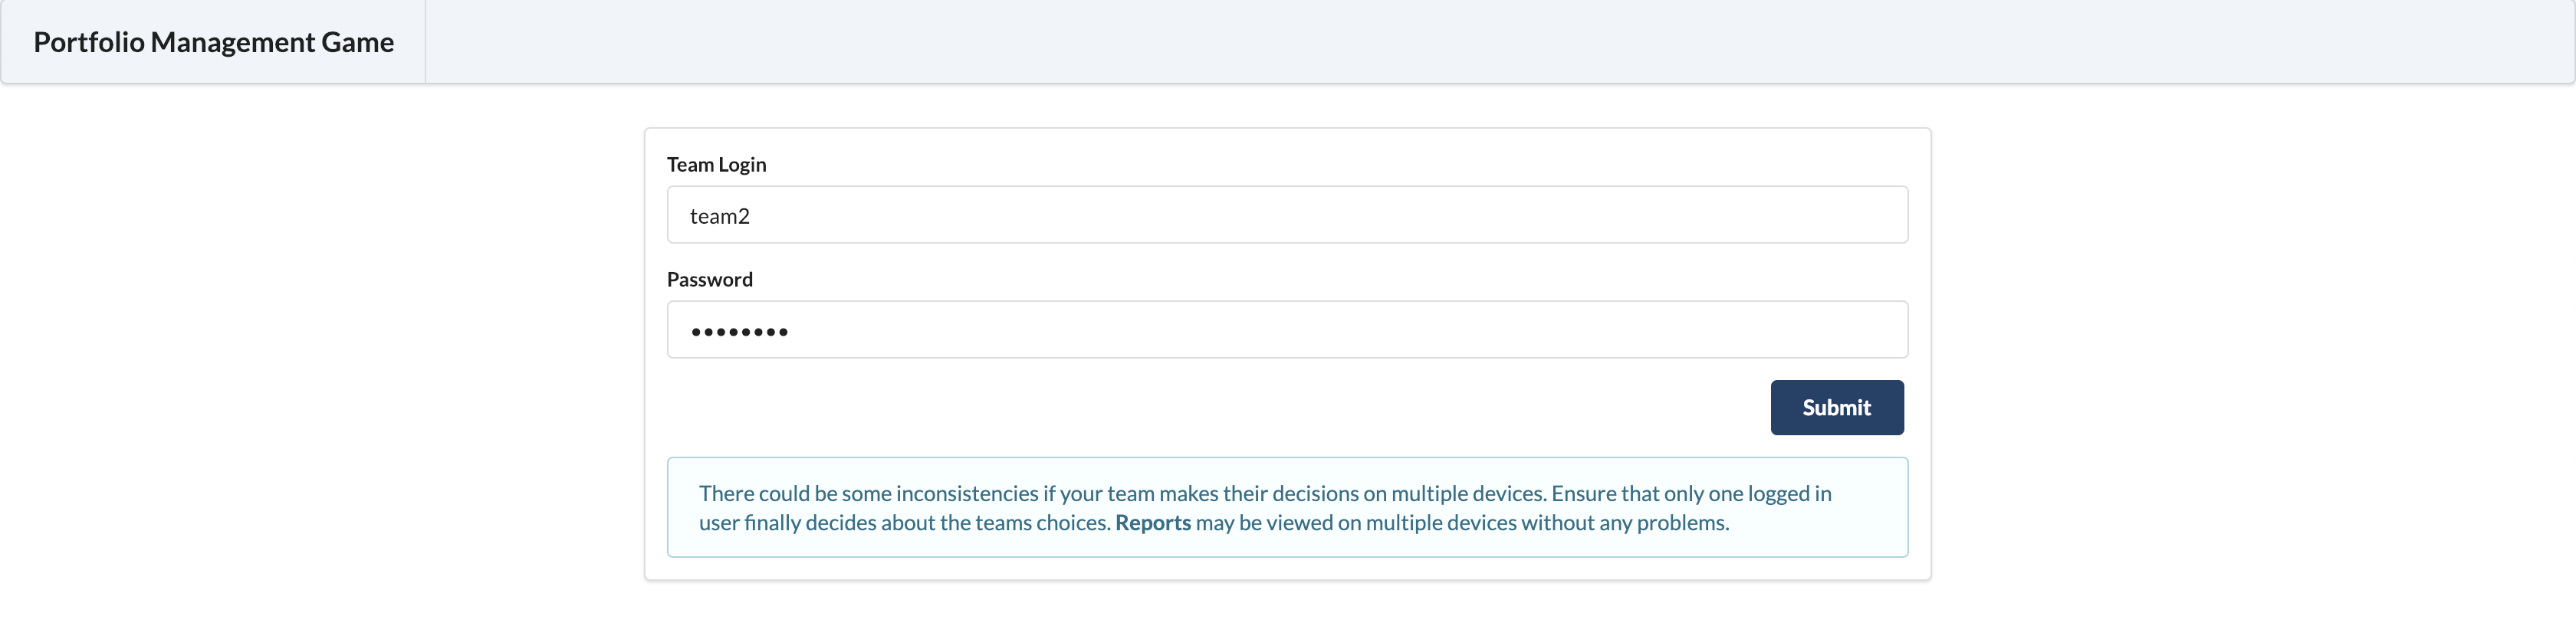
\includegraphics[scale=0.2]{img/application-overview/teams/01_login.png}
  \caption{Team login}
\end{figure}

\subsubsection{Period 0 decisions}
In period 0 which represents phase 1 of the game, the teams define their SAA for all customer types which are enabled by the administrator of the specific game. The teams need to fulfill the ranges for all dimensions to submit their decisions. Supportive graphs in form of pie charts help the teams to decide about the share of the two dimensions. Additionally, the players can name their team on the top left corner of the screen.
\begin{figure}[h!]
  \centering
  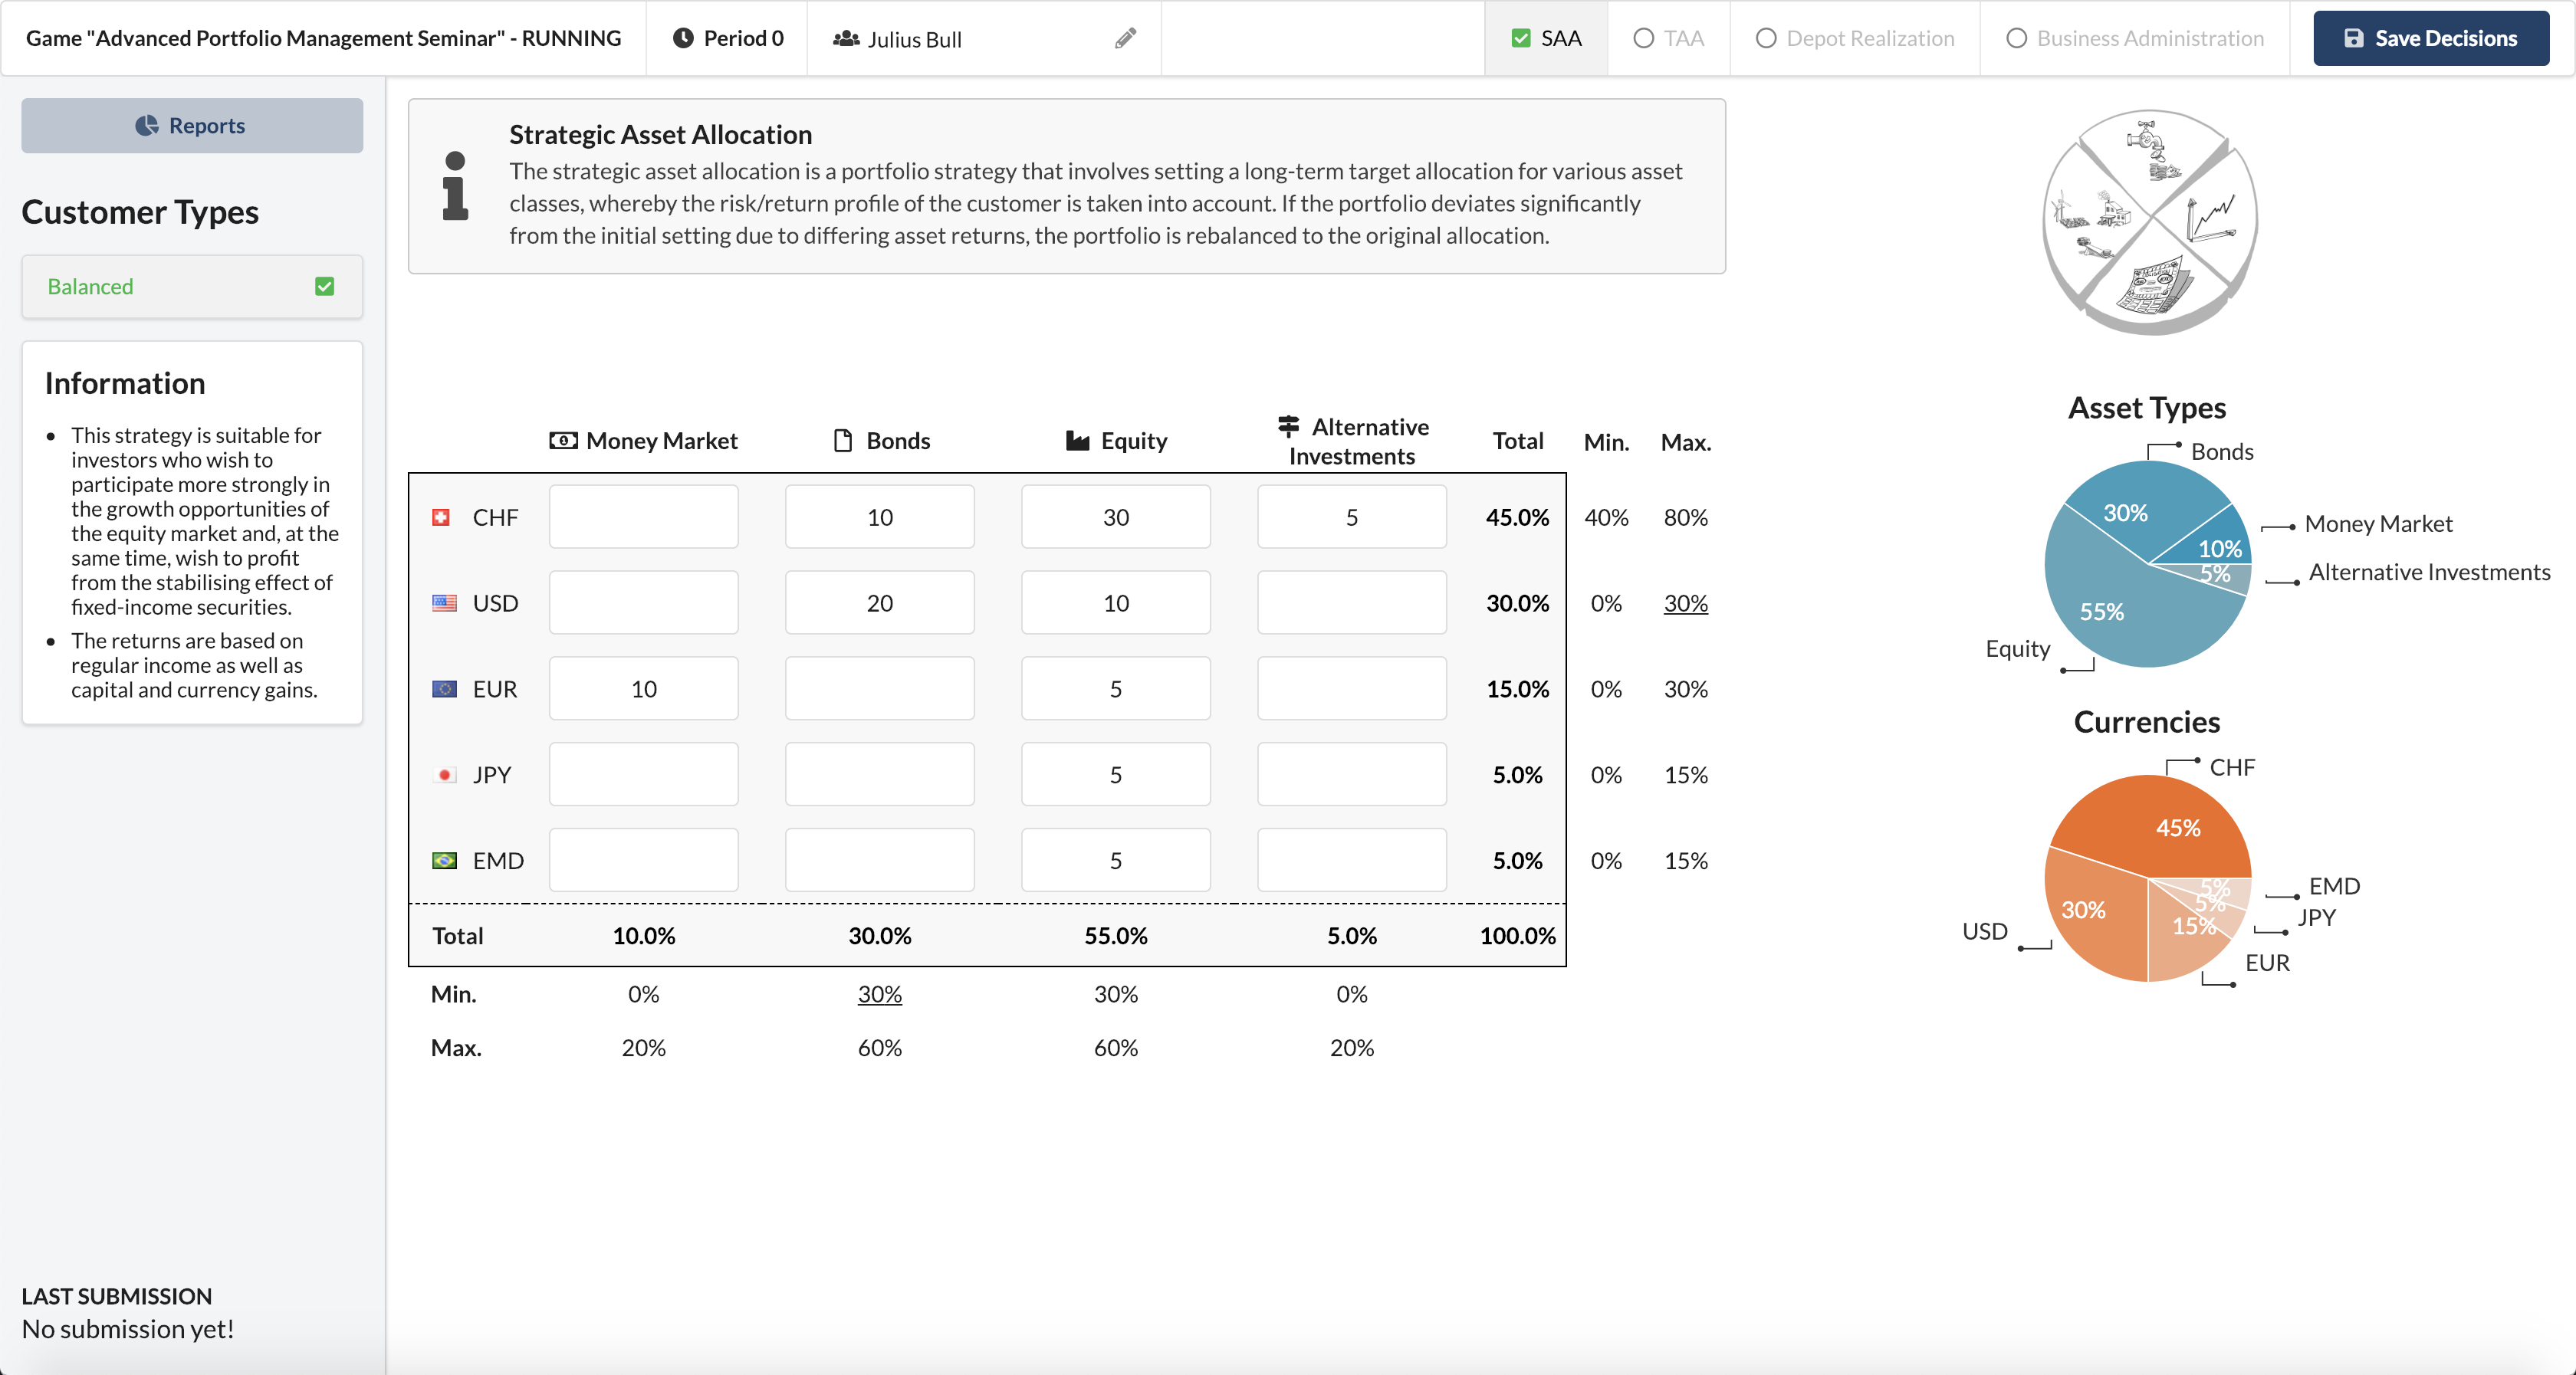
\includegraphics[scale=0.2]{img/application-overview/teams/02_period_zero_decisions.png}
  \caption{Period zero decisions}
\end{figure}

\subsubsection{Other periods decisions}
Starting from period 1, a team has to complete multiple decisions separated into four pages. Strategic asset allocation is fixed and not editable for a customer type which was defined at the beginning of the game. When the administrator defines a new customer type for an upcoming period, the teams have to allocate an SAA for the new customer type.\\

For each step within this process, a progress state helps the teams to understand the state of each step. For saving their decisions, all four steps have to be completed. In the bottom left corner, the submission state may be seen.

\paragraph{TAA}
For the tactical asset allocation, the teams can deviate from the SAA due to changes in the overall market. Equal to the strategic asset allocation screen the teams change the input within the table and get illustrative support with two graphs, displaying the allocations for both dimensions of the table. Initially, the inputs from the strategic asset allocation are loaded, whereas the students can adjust them to market changes. Arrows within the total summation of each asset type or currency show the status of being within the range.
\begin{figure}[h!]
  \centering
  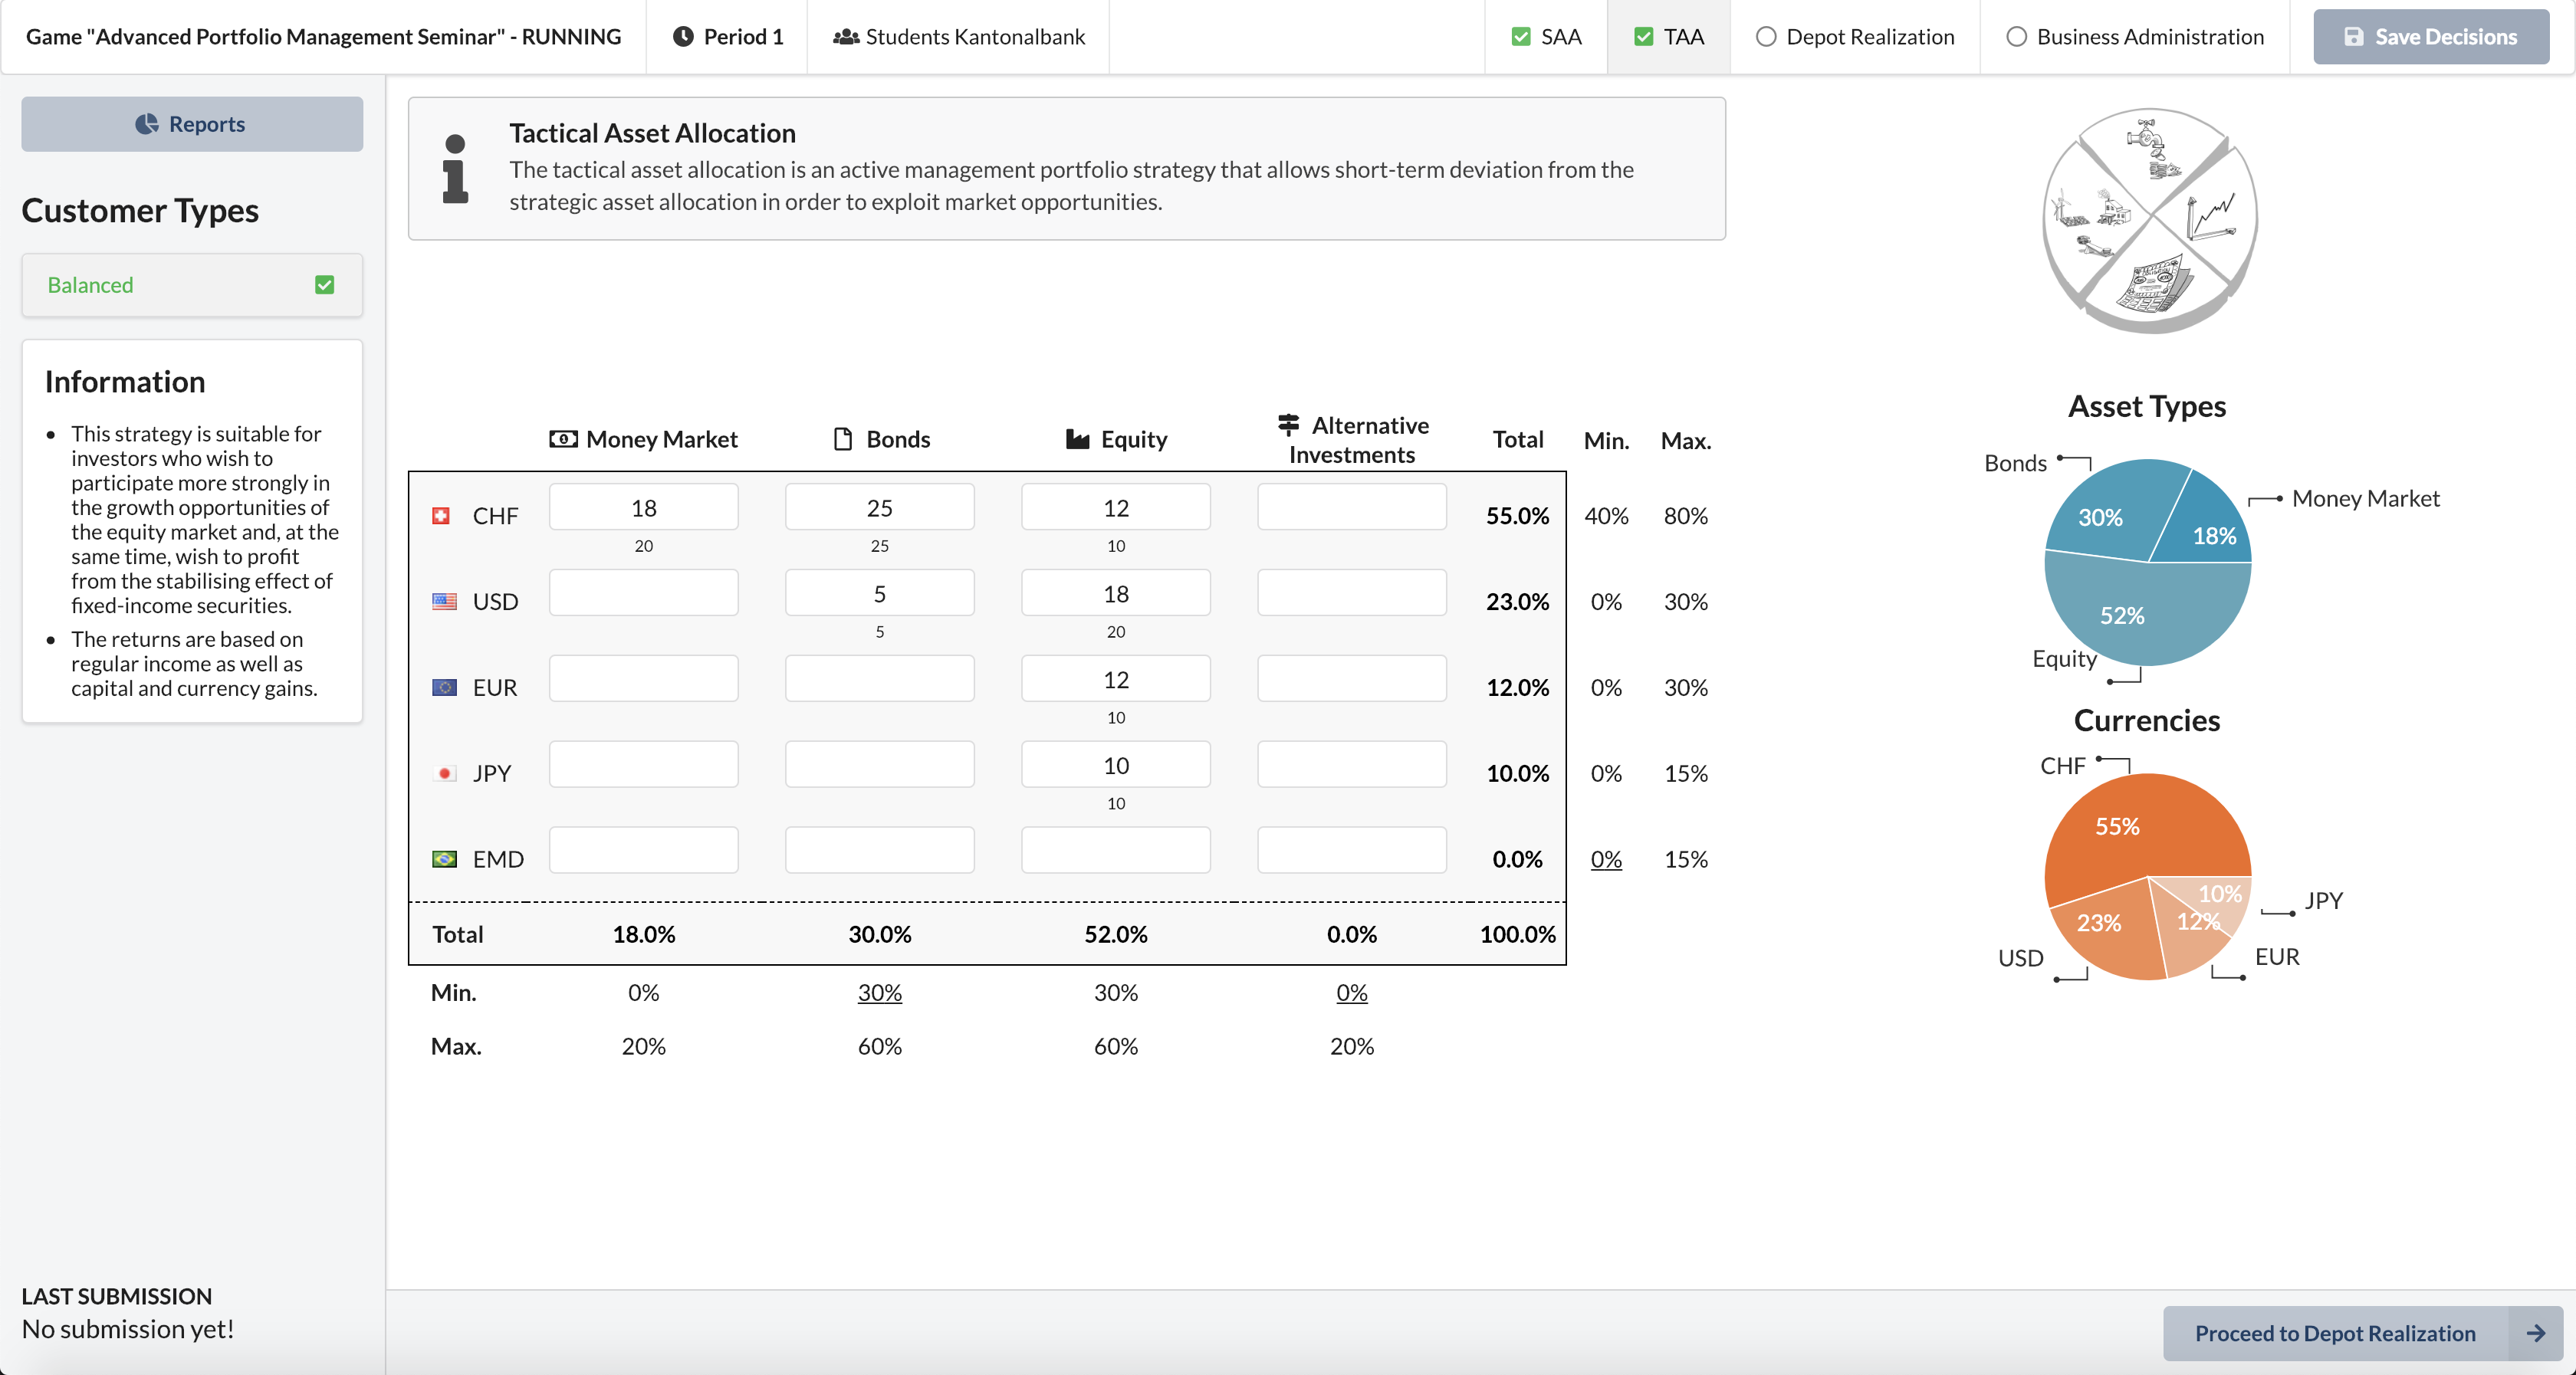
\includegraphics[scale=0.2]{img/application-overview/teams/04_taa.png}
  \caption{Tactical asset allocation}
\end{figure}

\paragraph{Depot Realization}
Based on SAA and TAA the teams finally have to allocate on specific assets. By having a bar chart on the top of the screen, students have an overview of their SAA and TAA decisions of the current active customer type. A target for the students is to allocate assets such that the yellow bar aligns with TAA for each asset type/currency combination. On the top right corner, a short summary of the most important key numbers for the allocations is present.
% TODO table description with filters etc.
This process has to be repeated for each customer type defined by navigating on the left menu. Equal to the SAA and TAA screen, the progress of the customer types is highlighted with checkmarks and corresponding colors.

\begin{figure}[h!]
  \centering
  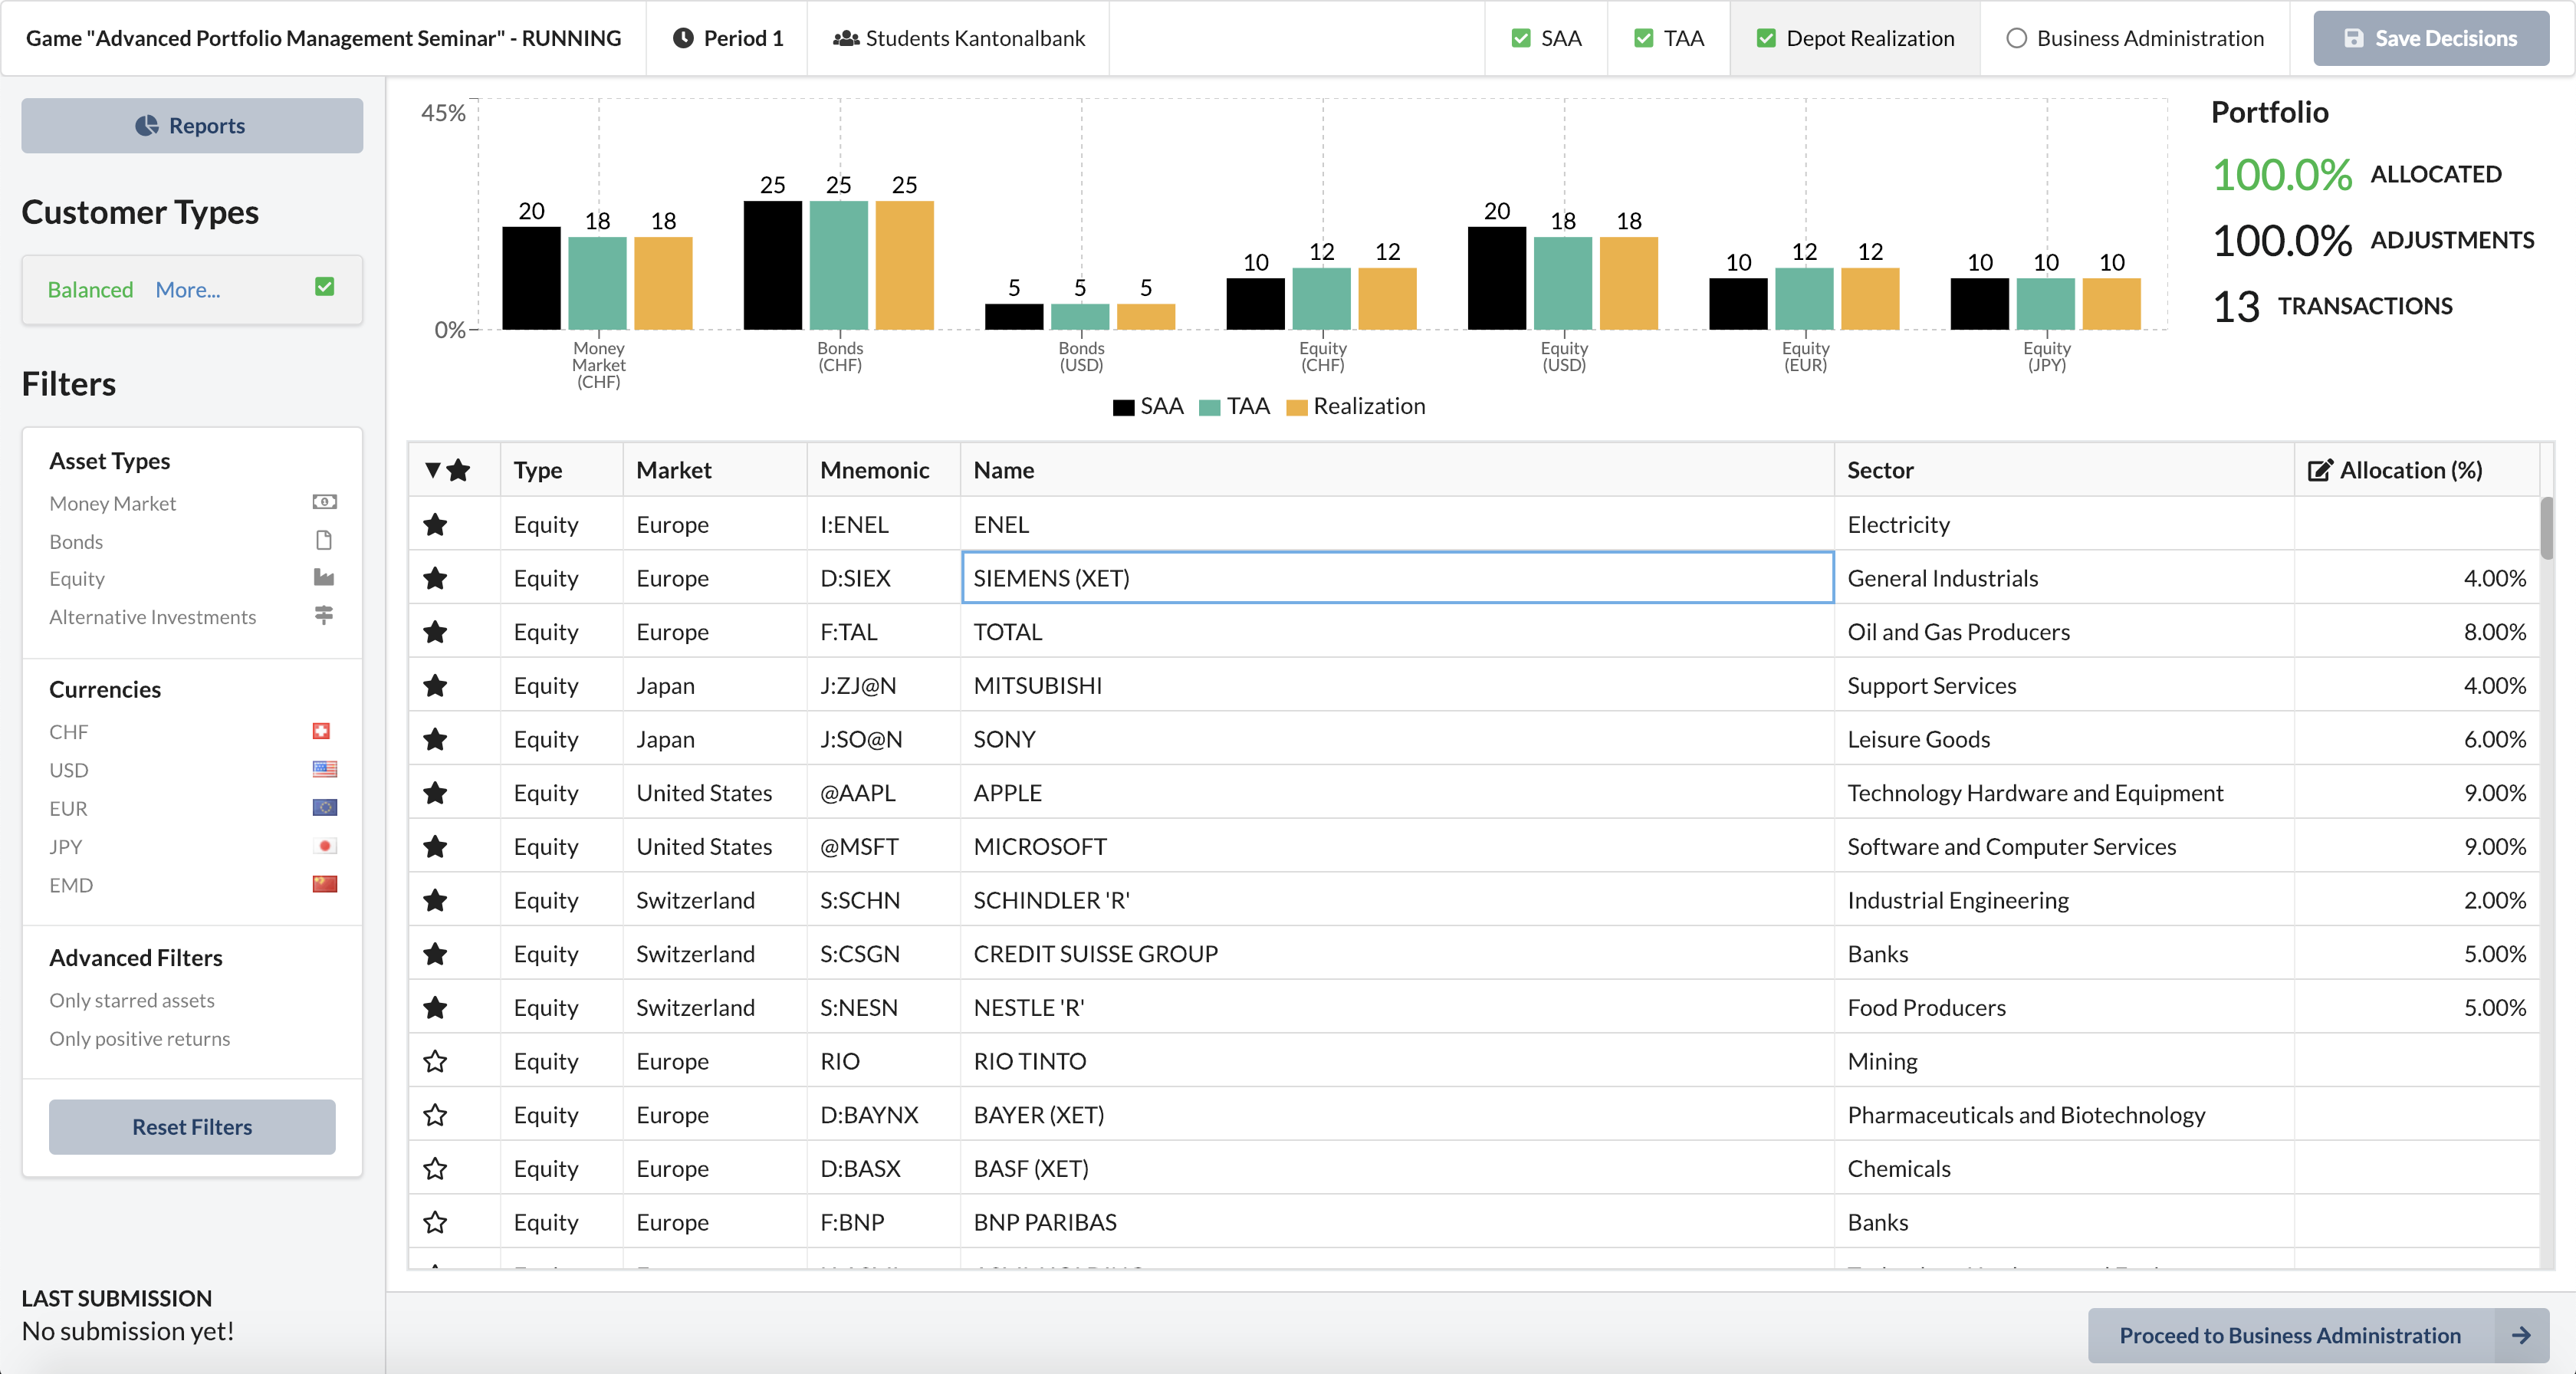
\includegraphics[scale=0.2]{img/application-overview/teams/05_depot_realization.png}
  \caption{Depot realization}
\end{figure}

\paragraph{Business Administration}
Business administration operates as the final decisions for a period. On the left side of the screen teams input numbers for four different categories: Conditions \& Fees, Human resources, logistics, and profit distribution. For each input field, the initial value (in period 1) or the previous period value (for all other periods) is displayed next to the input field.\\

On the right side, the balance sheet from the previous period is visualized to inform teams about their business results. Further key information is displayed on top of the balance sheet.
\begin{figure}[h!]
  \centering
  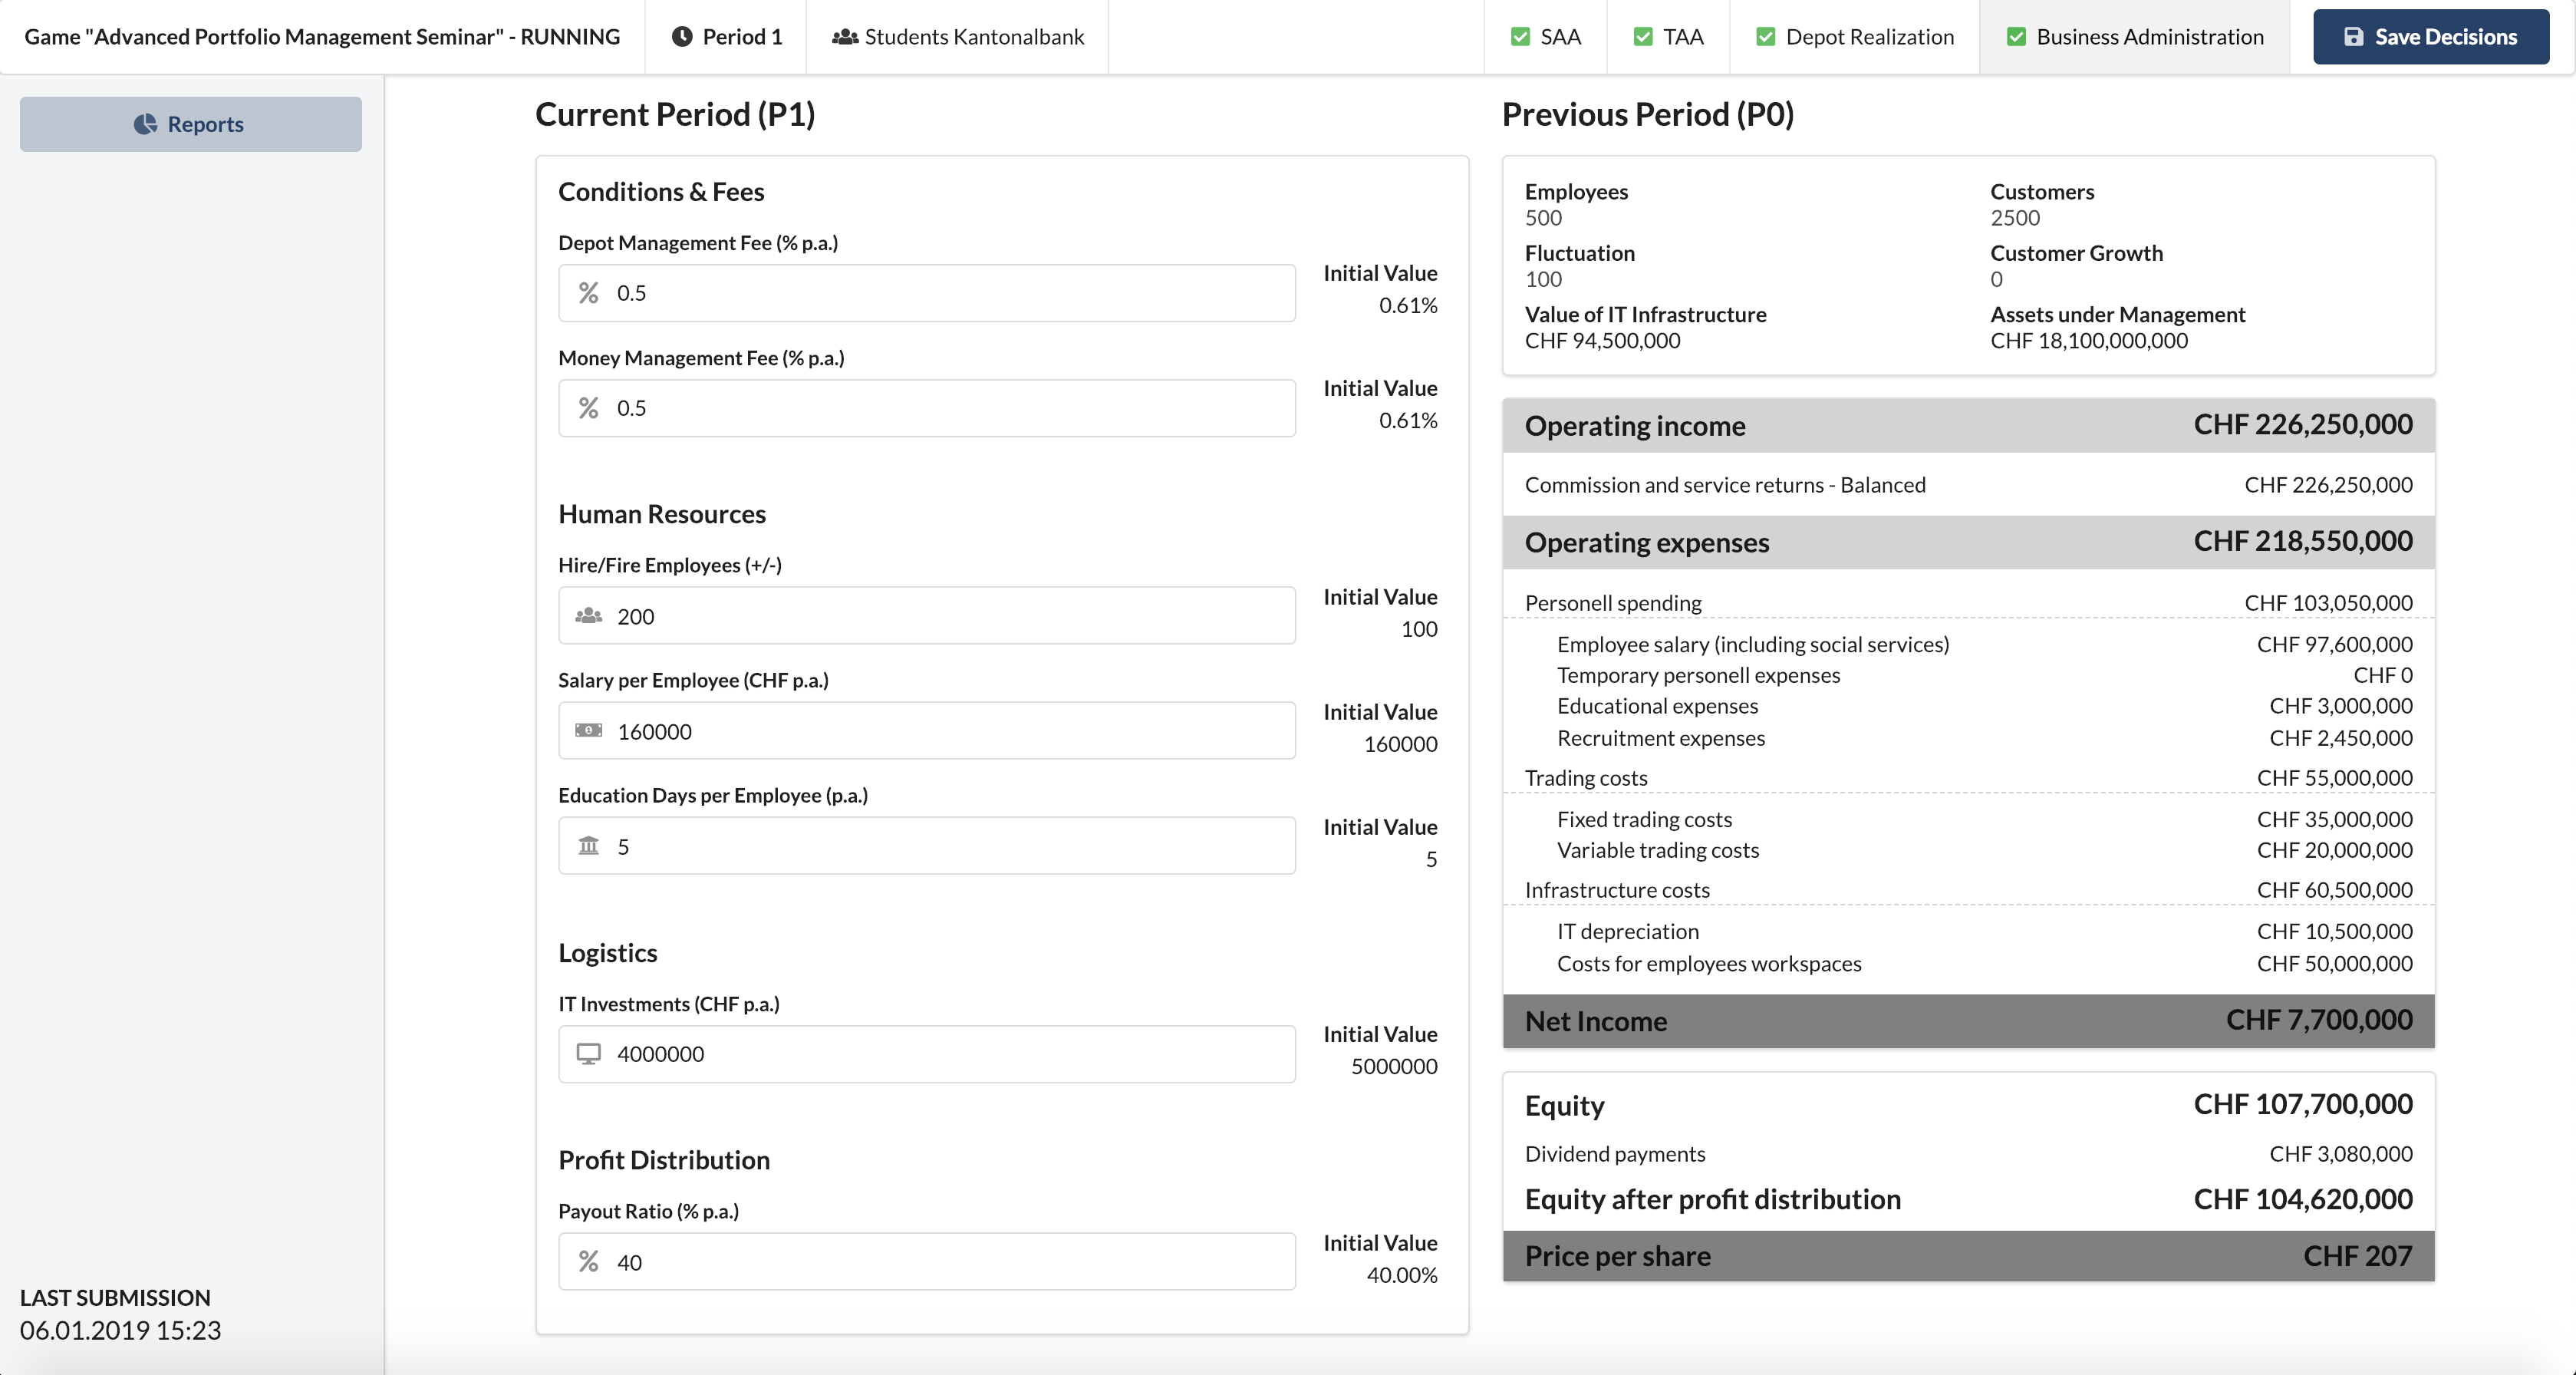
\includegraphics[scale=0.2]{img/application-overview/teams/06_business.png}
  \caption{Business administration}
\end{figure}

\subsection{Reports}
Reports are available for both administrators of a game and teams. They explain the results of the different periods of each team and compare them to the results of the other teams. As there are many graphs available, they are structured into multiple tabs, which will be explained within this subsection. The report section may be filtered by team and by periods.

\subsubsection{Overview}
A short overview sets up the report page. A two-dimensional comparison between performance and total earnings should summarize up the investment profits of the teams, where each point represents a team at a specific period. The stock price development of the different teams shows the progress of the stock price over all periods. The best performing team concludes the last period of the game with the highest stock price. On the bottom of those graphs, there is a spider chart for each team describing indexes within a range of 0 to 10.
\begin{figure}[h!]
  \centering
  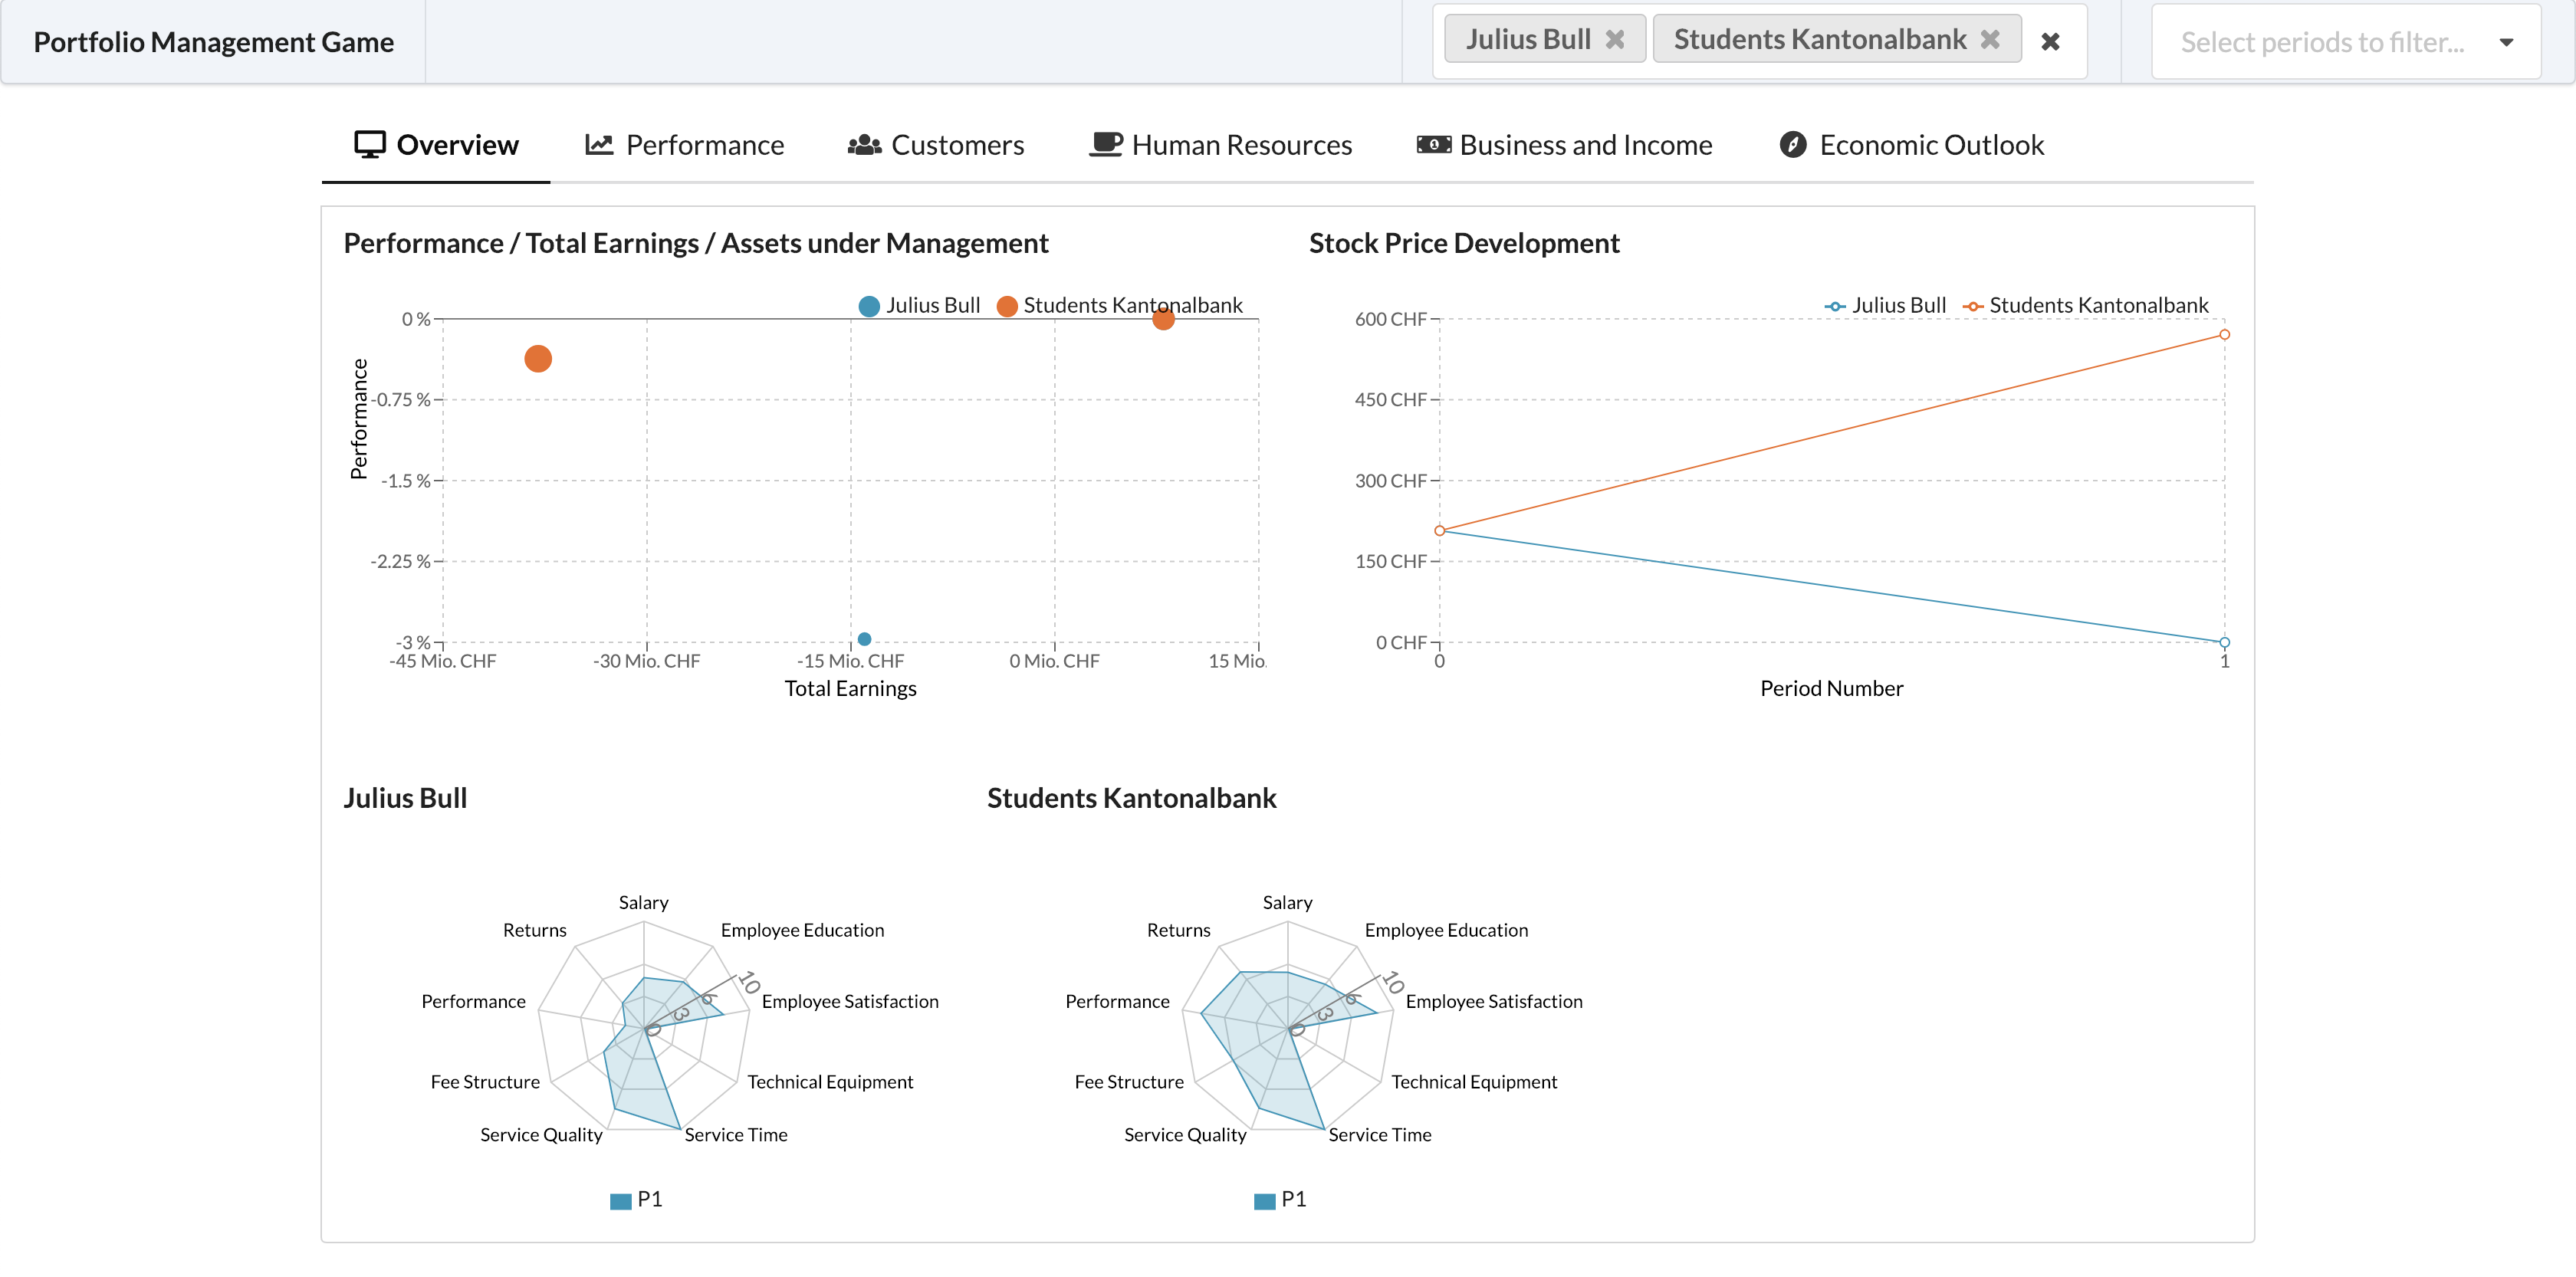
\includegraphics[scale=0.2]{img/application-overview/reports/01_overview.png}
  \caption{Reports - Overview}
\end{figure}

\subsubsection{Performance}
Multiple bar charts describe the performance of the teams for each customer type in each period. Such as:
\begin{itemize}
  \setlength\itemsep{0.01em}
  \item Portfolio returns
  \item Sharpe ratio
  \item Traynor ratio
  \item Jensen's alpha
  \item Information ratio
\end{itemize}
\begin{figure}[h!]
  \centering
  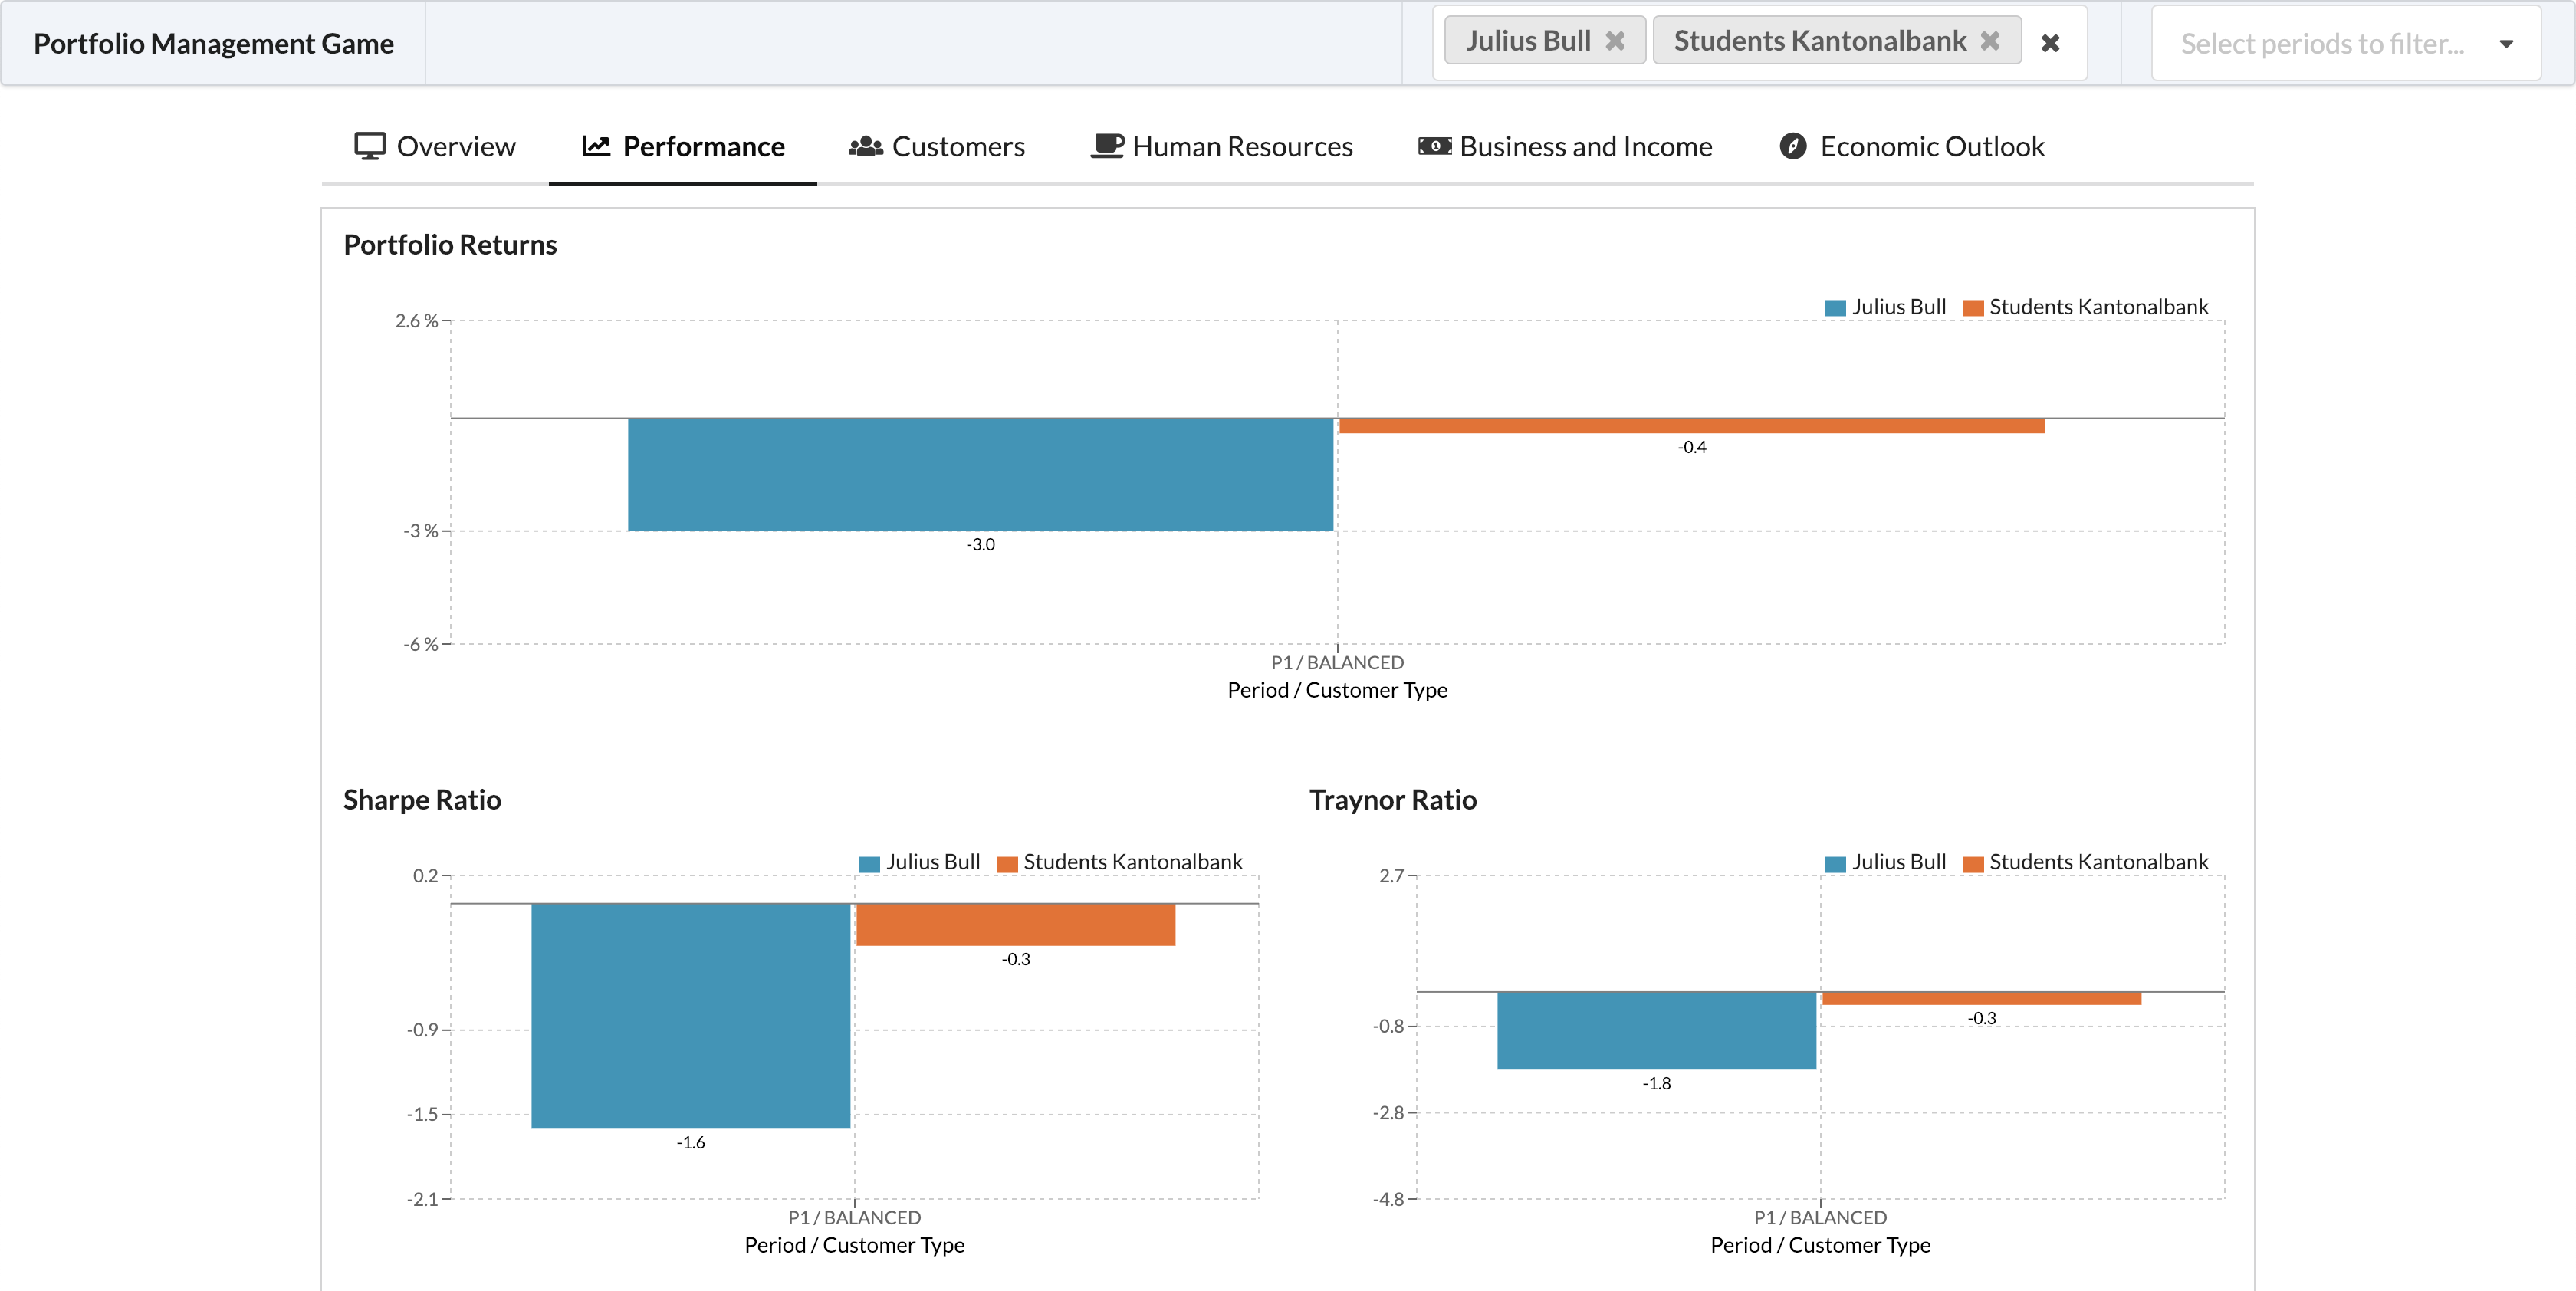
\includegraphics[scale=0.2]{img/application-overview/reports/02_performance.png}
  \caption{Reports - Performance}
\end{figure}

\subsubsection{Customers}
Similar to the performance tab, the customer section explains multiple key characteristics of customers for each team and period.
\begin{itemize}
  \setlength\itemsep{0.01em}
  \item Customer satisfaction index
  \item Number of Customers
  \item Customer growth
  \item Assets under management
  \item Net new money
  \item Relative TAA discrepancy (volume-weighted)
  \item Number of SAA violations
\end{itemize}
\begin{figure}[h!]
  \centering
  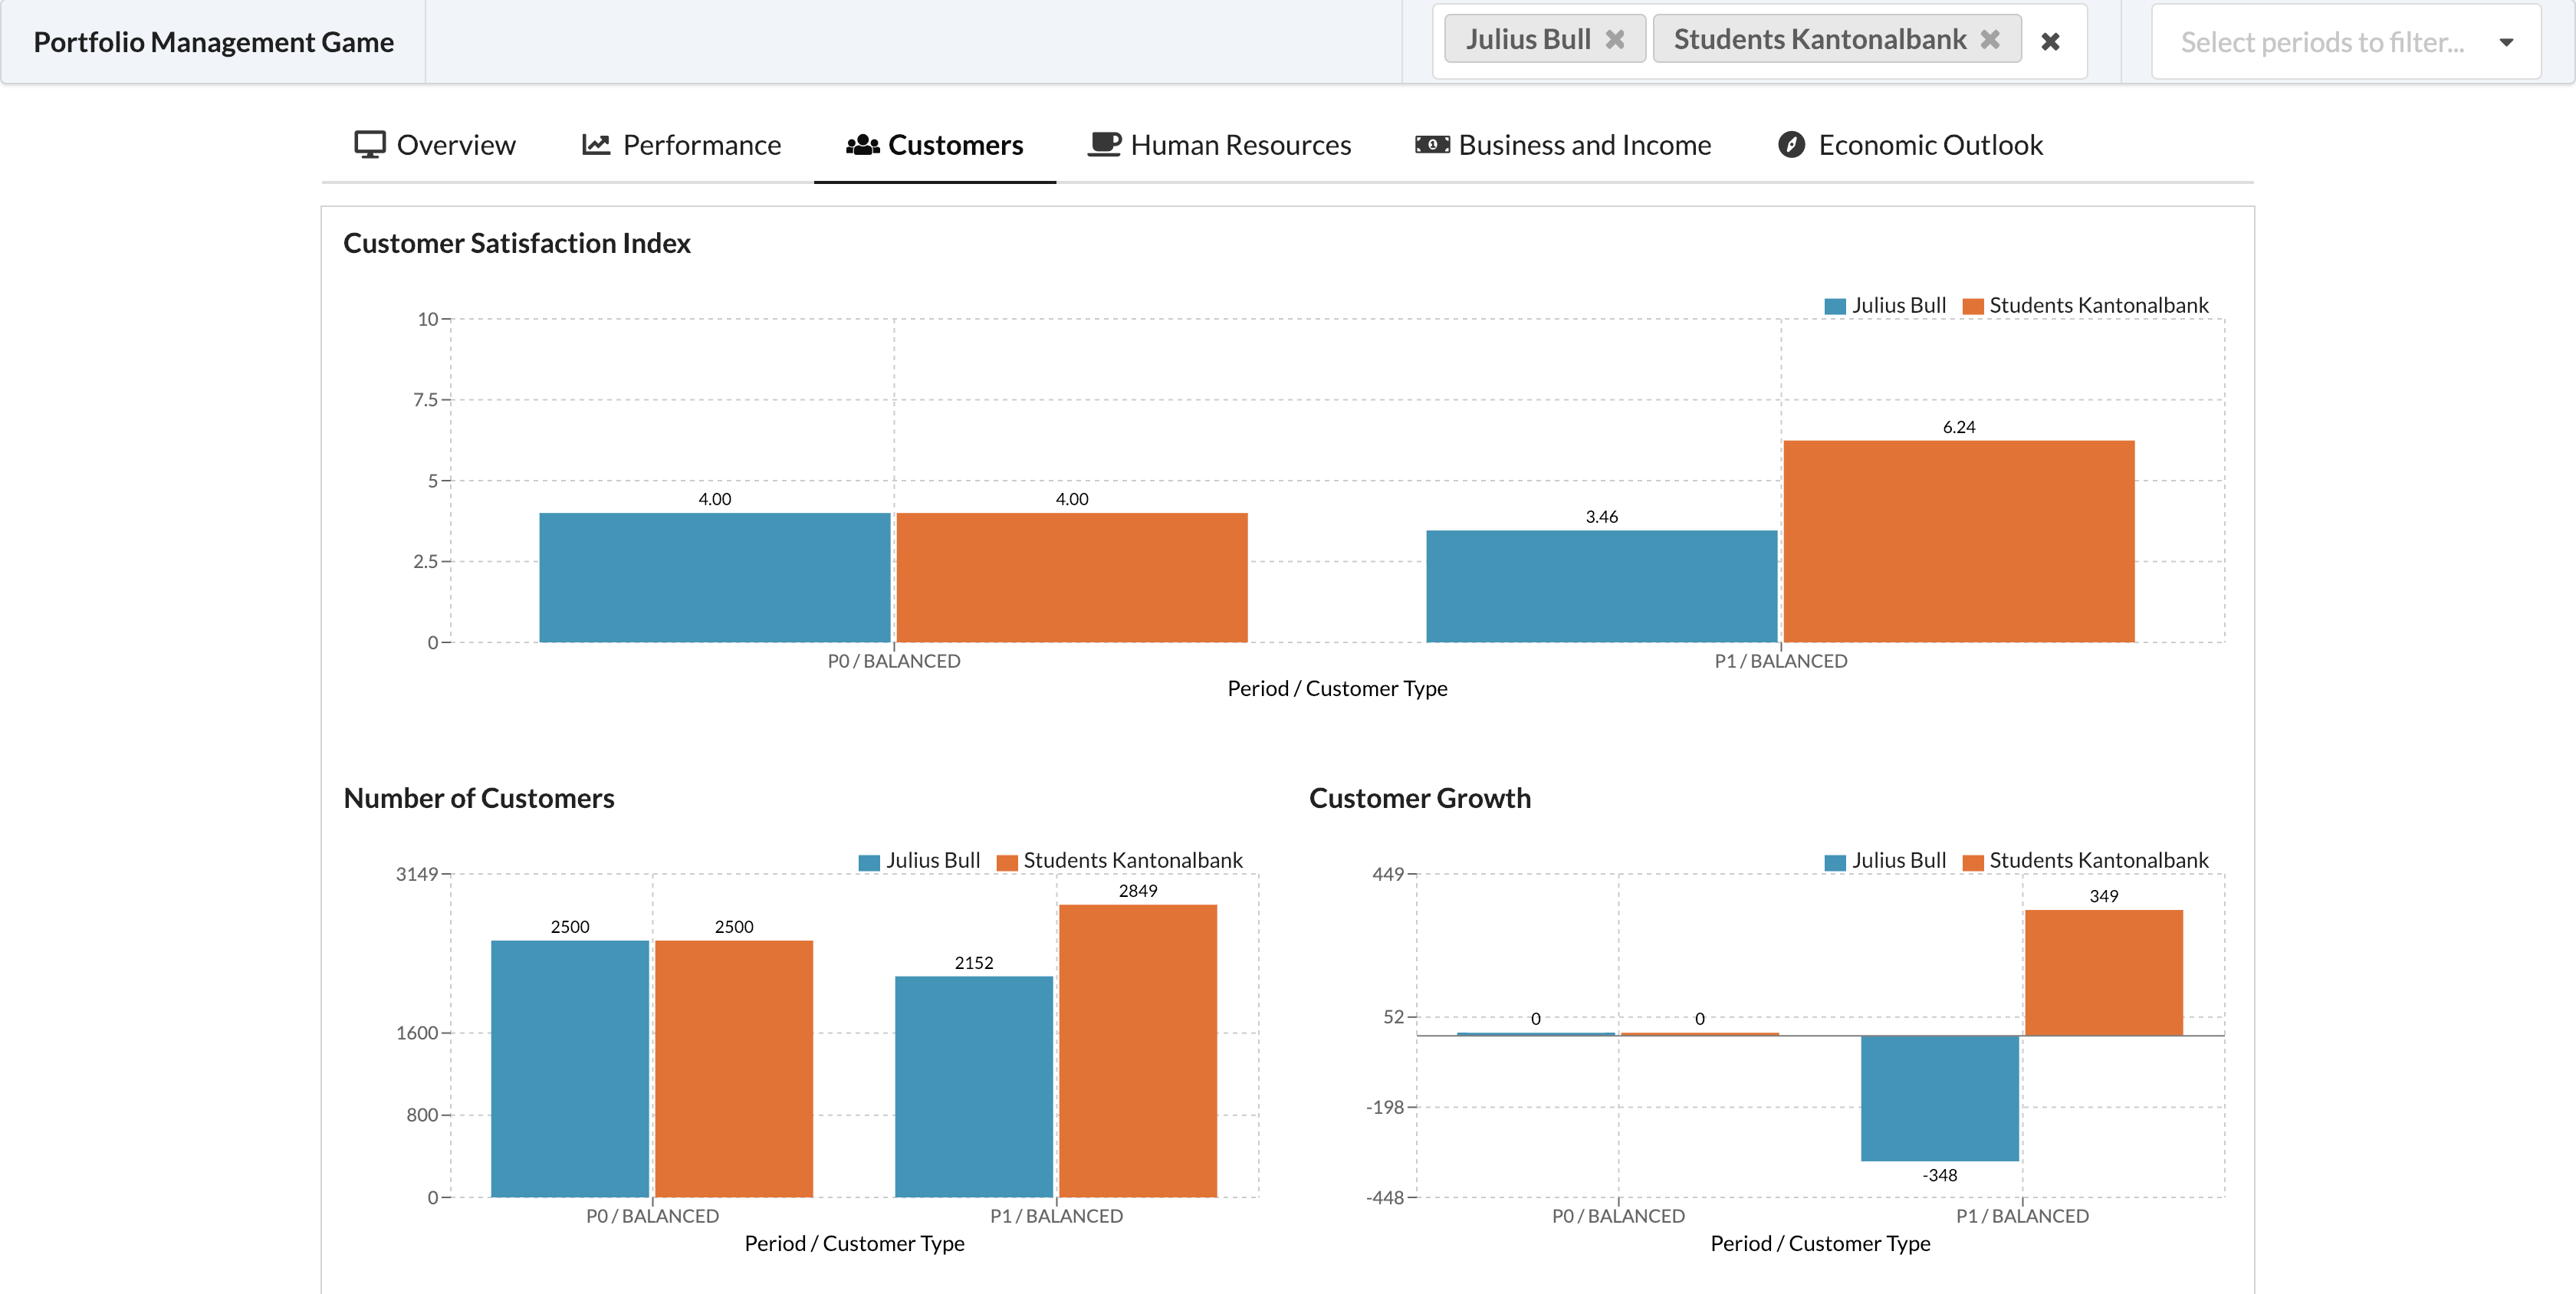
\includegraphics[scale=0.2]{img/application-overview/reports/03_customers.png}
  \caption{Reports - Customers}
\end{figure}

\subsubsection{Human ressources}
Information about human resources (HR) is displayed using four bar charts:
\begin{itemize}
  \setlength\itemsep{0.01em}
  \item Employee satisfaction index
  \item Number of employees
  \item Salary index
  \item Education index
\end{itemize}
\begin{figure}[h!]
  \centering
  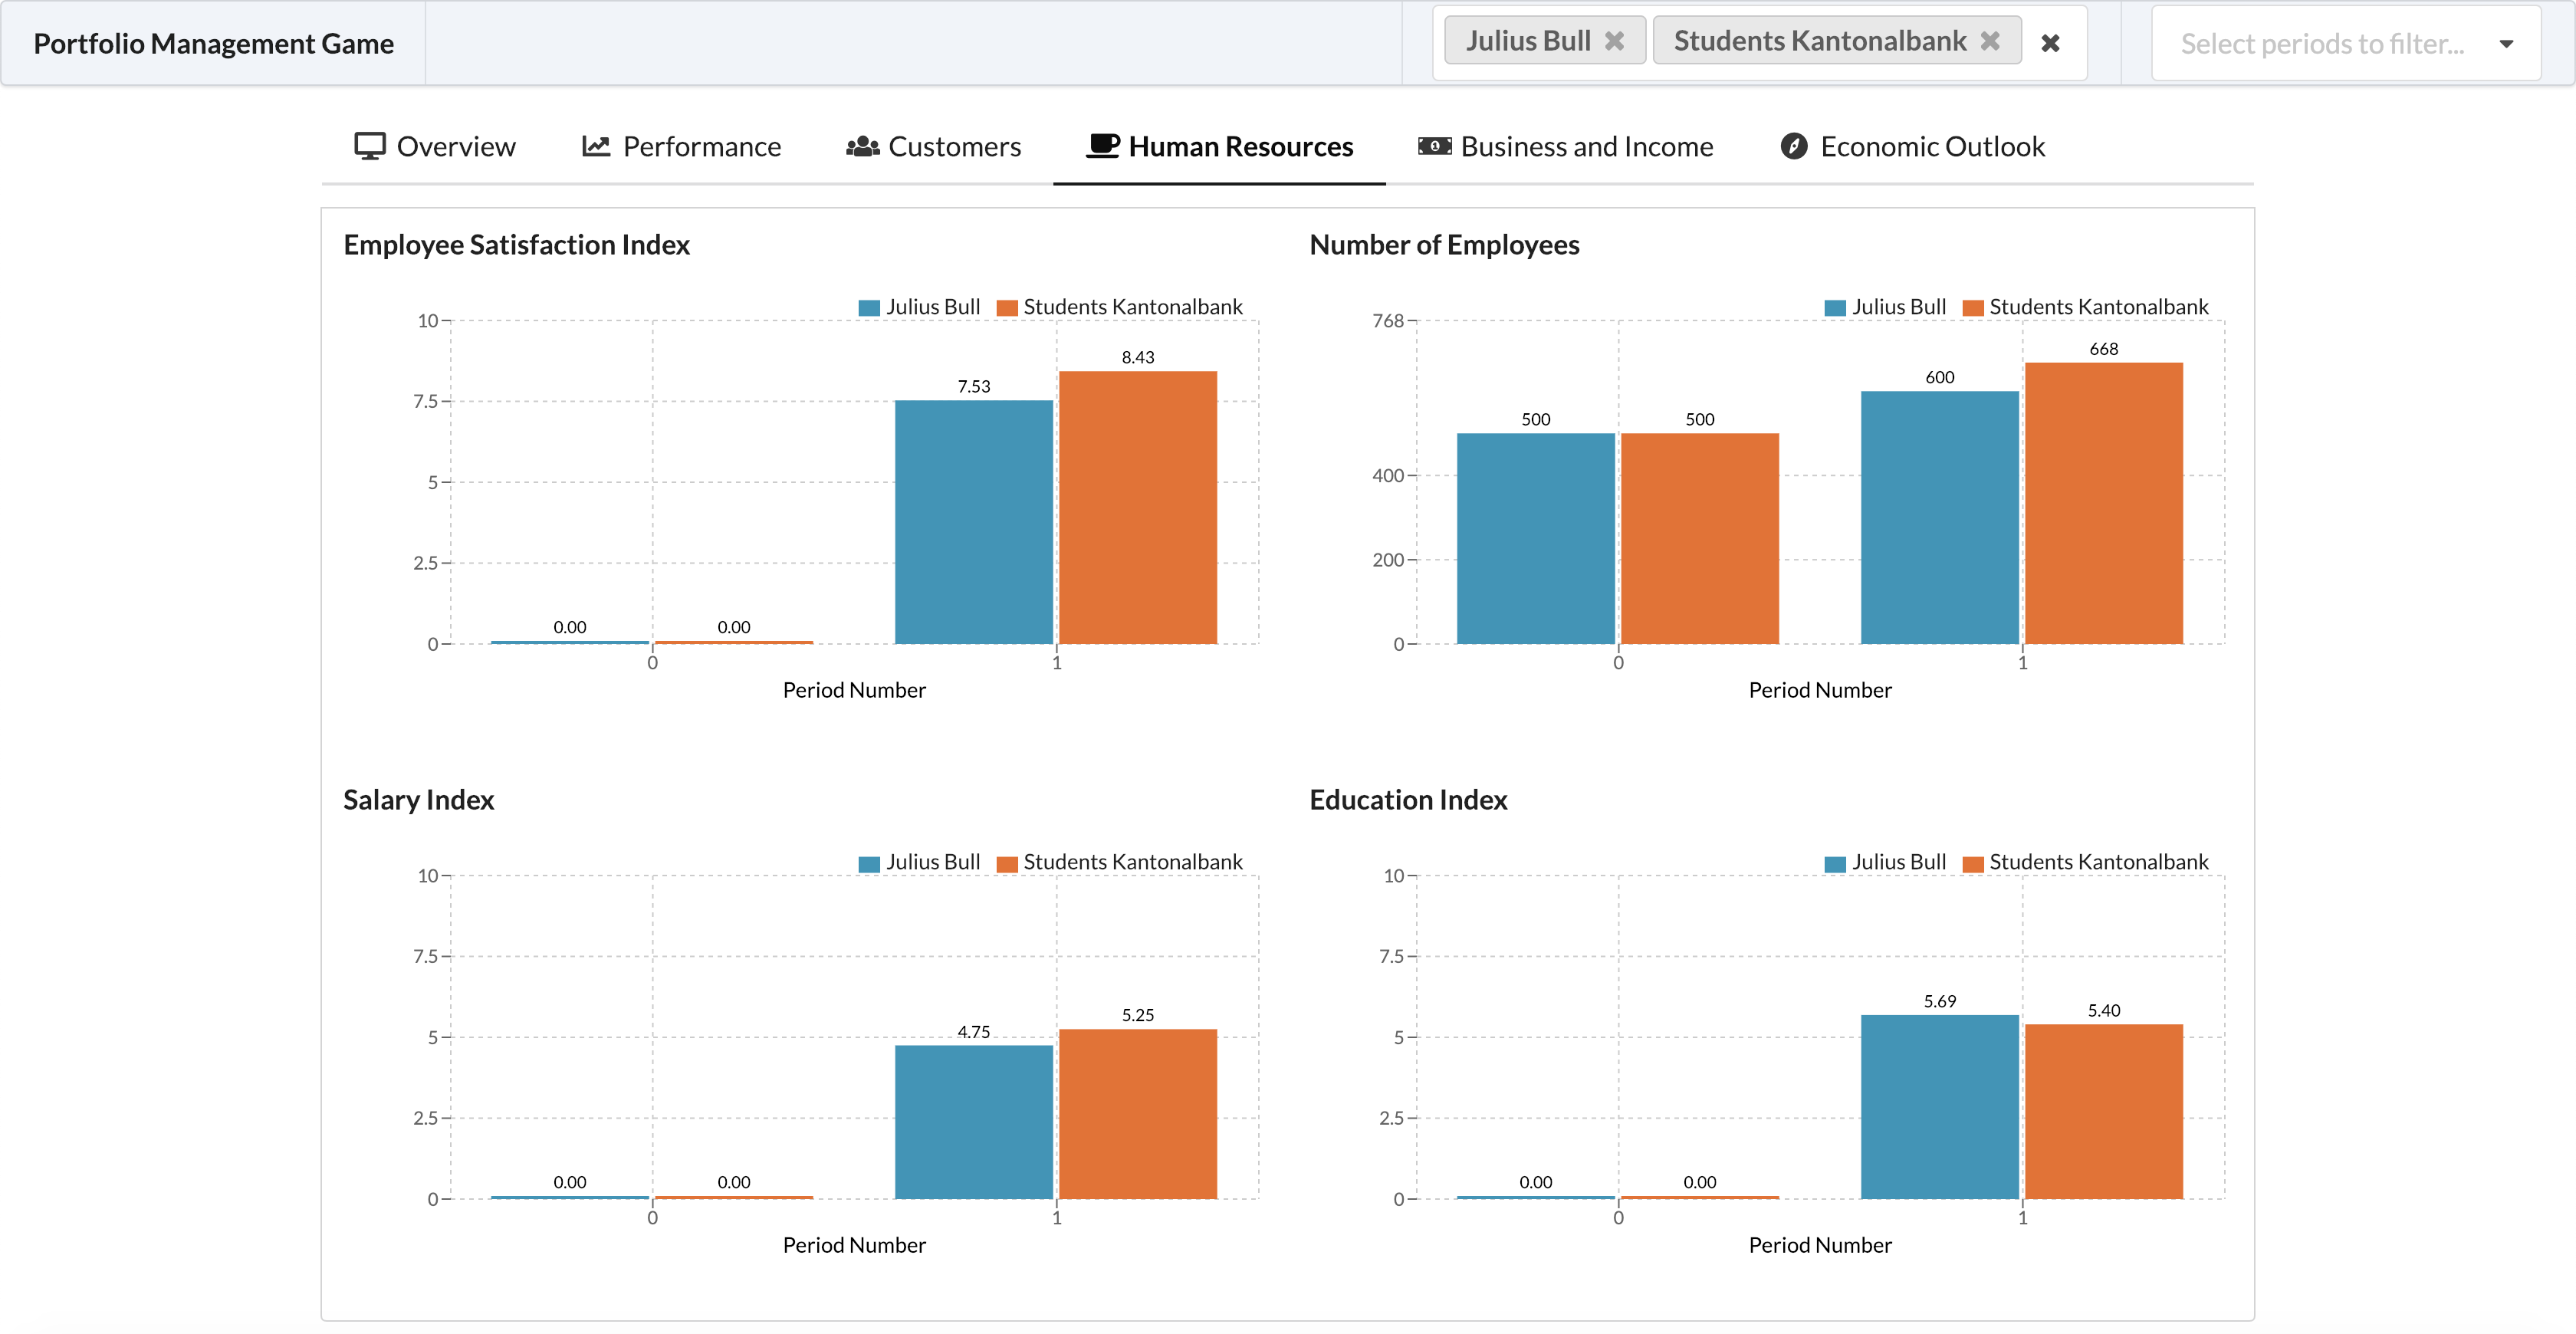
\includegraphics[scale=0.2]{img/application-overview/reports/04_hr.png}
  \caption{Reports - Human ressources}
\end{figure}

\subsubsection{Business and Income}
Starting with four bar charts this tab explains about business decisions:
\begin{itemize}
  \setlength\itemsep{0.01em}
  \item Operating Income
  \item Operating expenses
  \item Cost income ratio
  \item Net Income
\end{itemize}
\begin{figure}[h!]
  \centering
  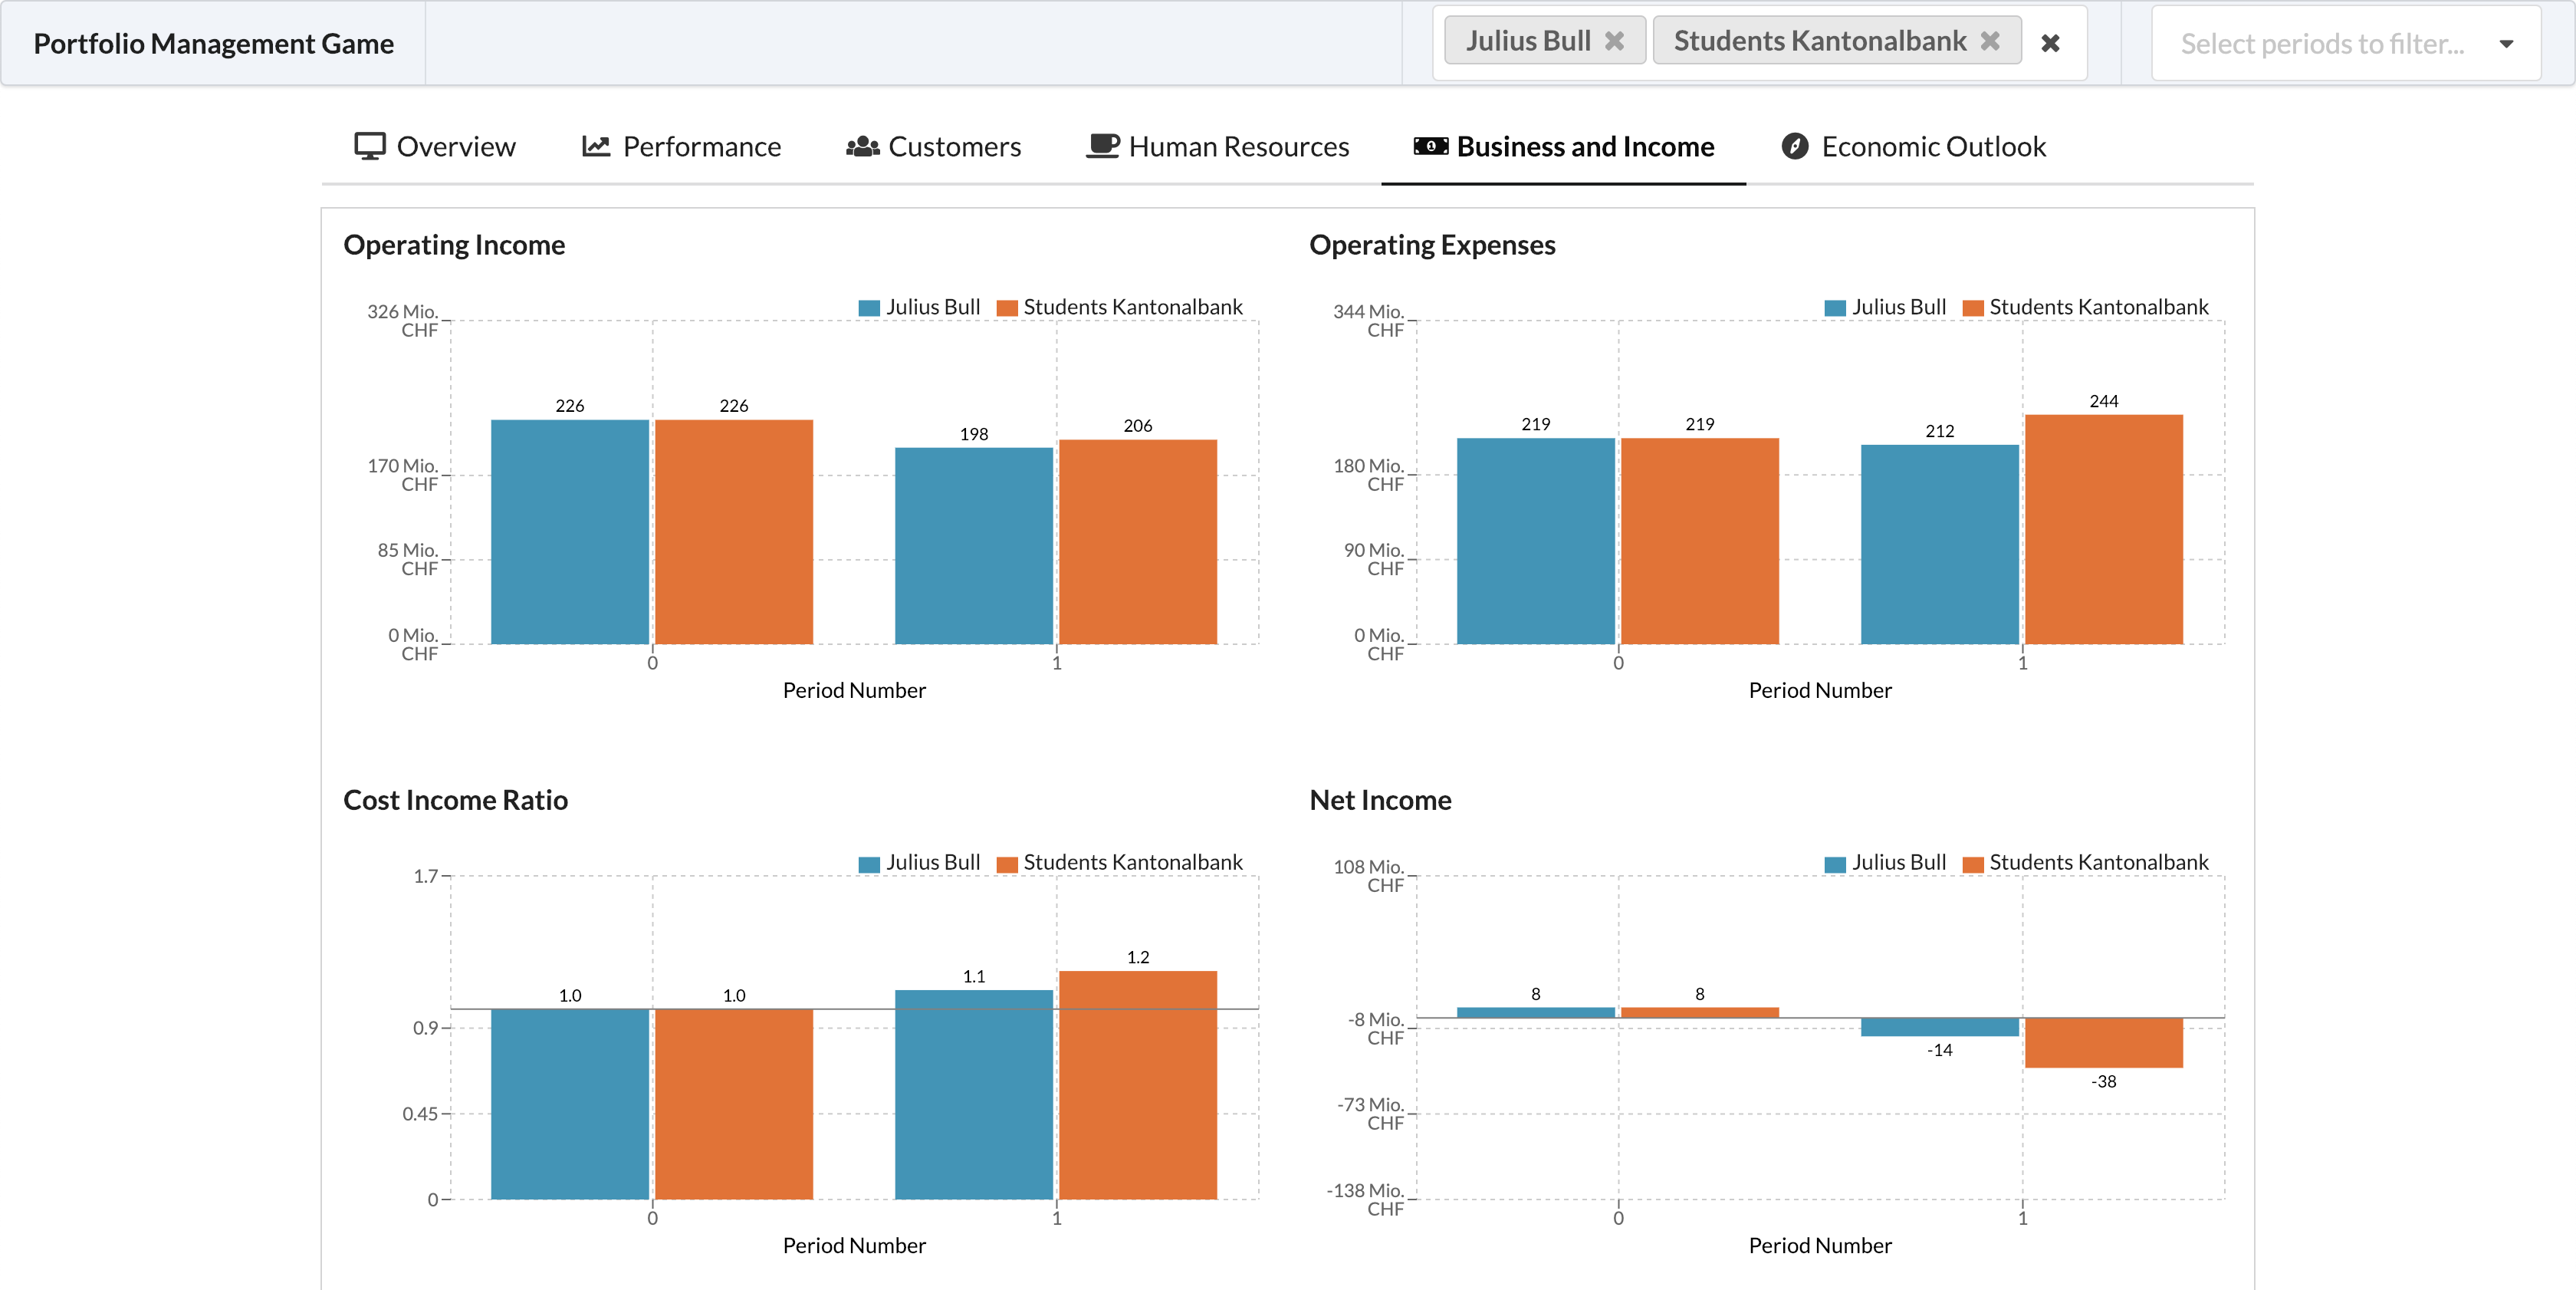
\includegraphics[scale=0.2]{img/application-overview/reports/05_business_income.png}
  \caption{Reports - Business and Income}
\end{figure}

In figure \ref{fig:reports_balance_sheet_comparison} different teams in different periods can be compared for their balance sheet. The users can either compare previous periods with upcoming of their own balance sheet or compare their own result to other teams in the same period.
\begin{figure}[h!]
  \centering
  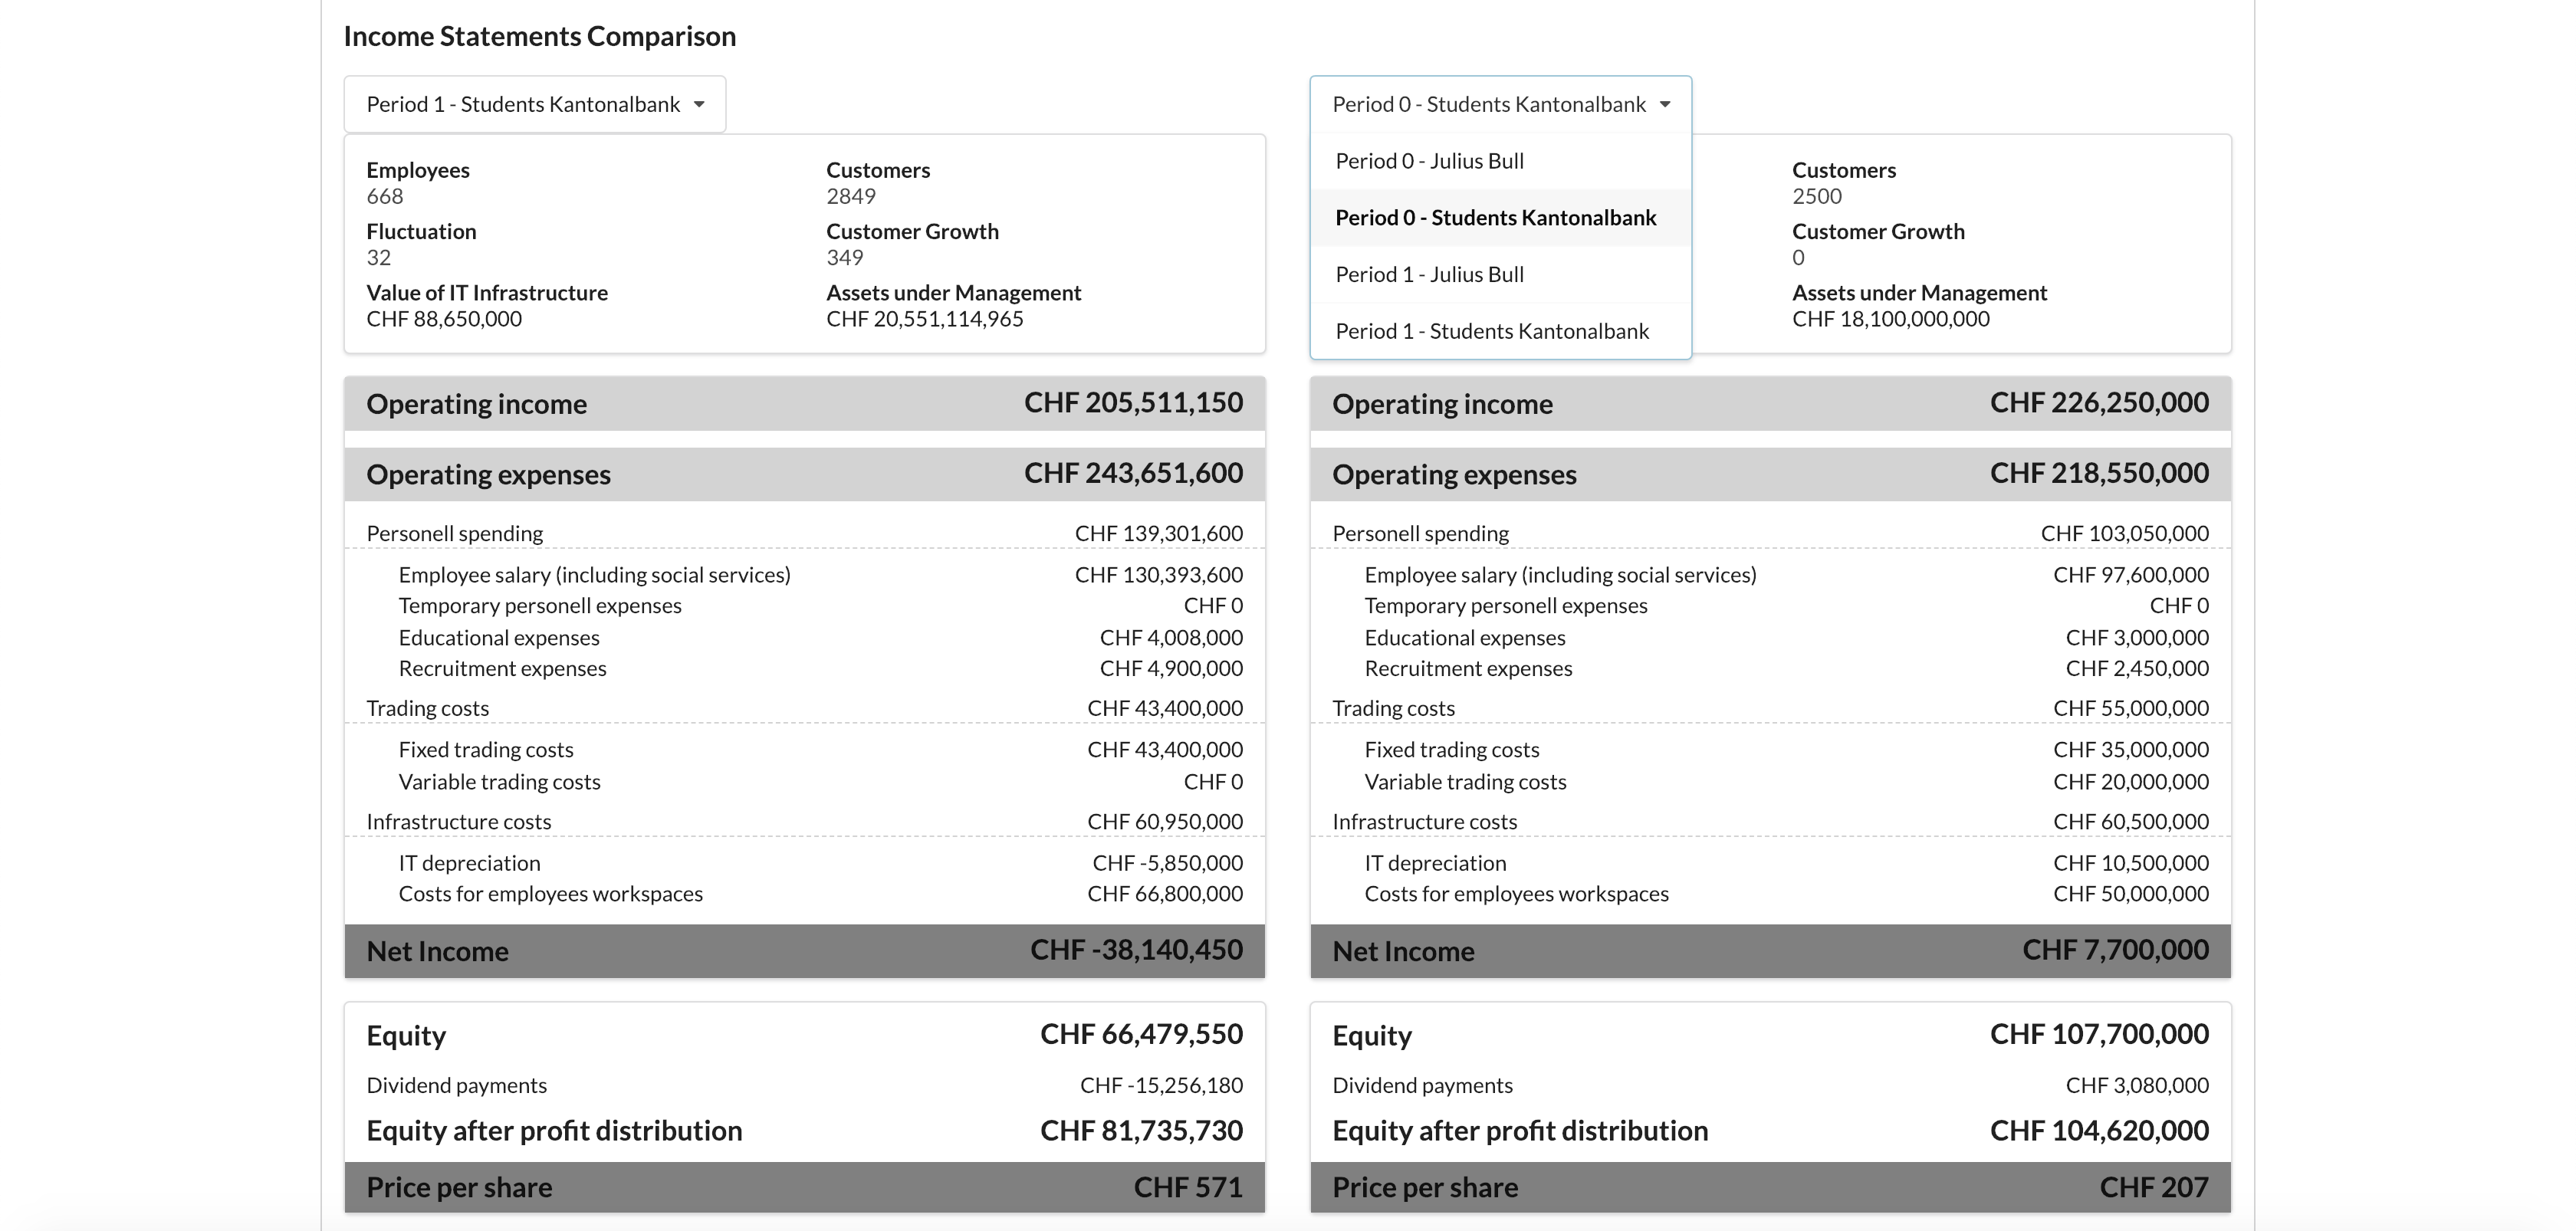
\includegraphics[scale=0.2]{img/application-overview/reports/05_business_income_balance_sheet_comparison.png}
  \caption{Reports - Balance sheet comparison}
  \label{fig:reports_balance_sheet_comparison}
\end{figure}


\subsubsection{Economic Outlook}
The economic outlook is the only tab, which is already accessible from period 1, as all other graphs or tabs have to be in at least period 2 because the first actual decisions (except for the saa) take place in period 1.
\begin{figure}[h!]
  \centering
  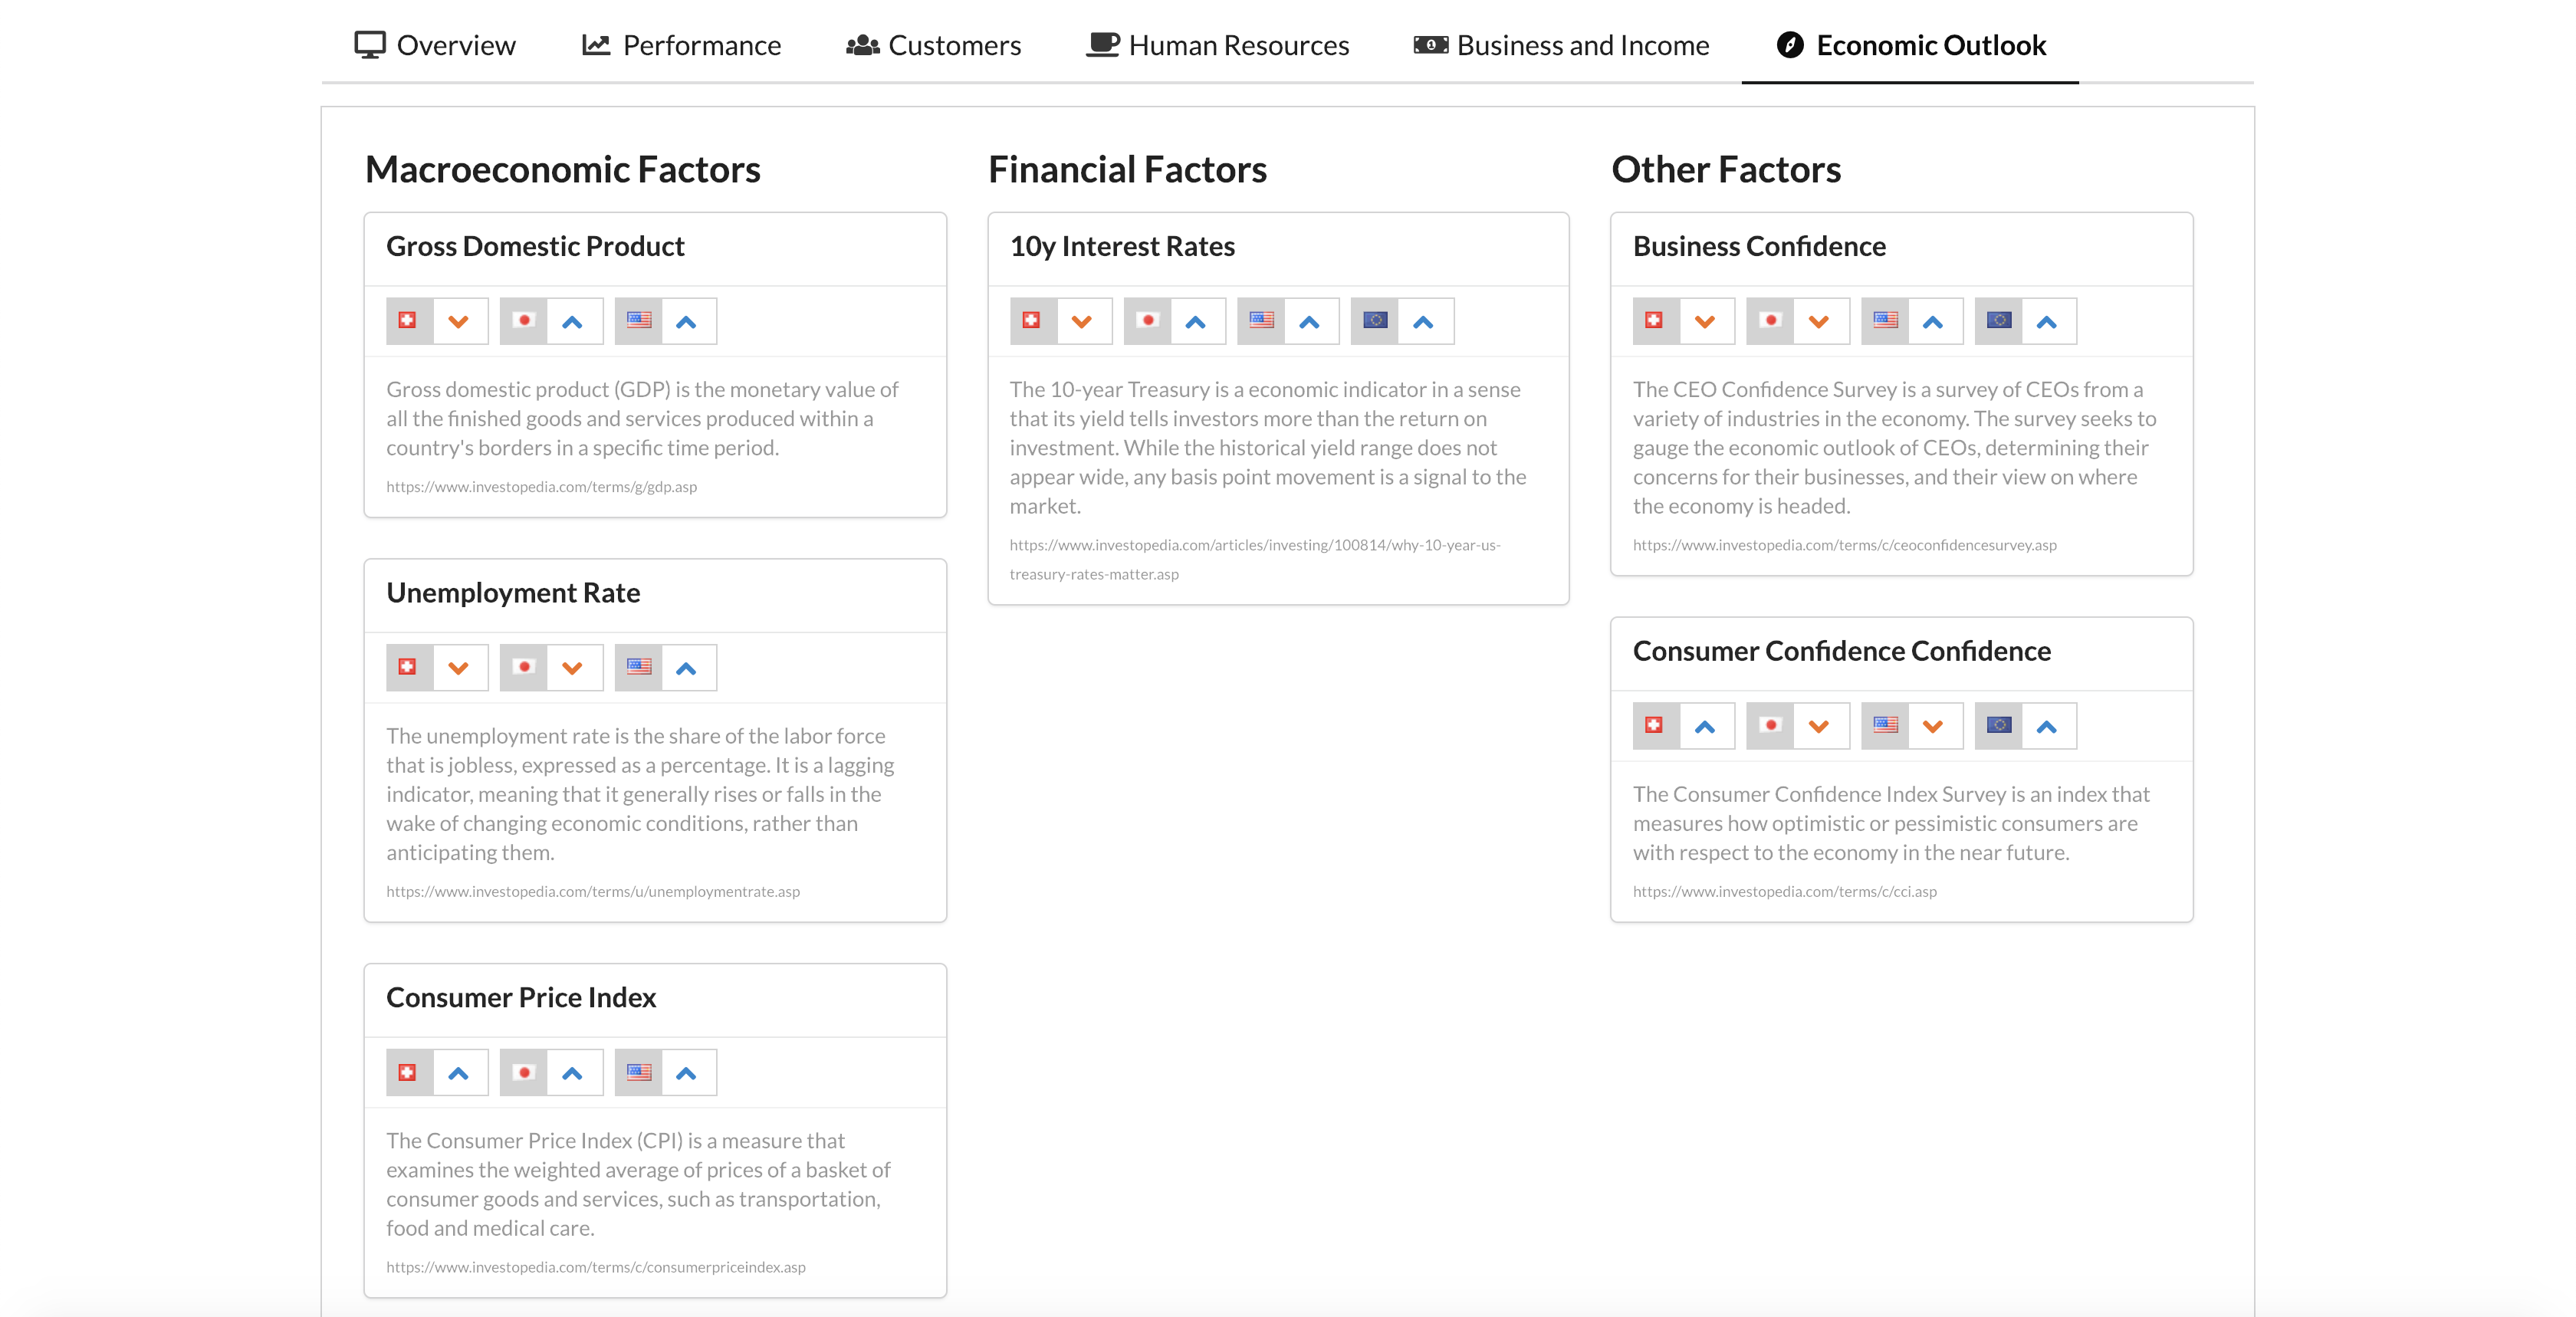
\includegraphics[scale=0.2]{img/application-overview/reports/06_economic_outlook.png}
  \caption{Reports - Economic outlook}
\end{figure}
